\documentclass[
  a4paper,BCOR10mm,oneside,
  headsepline,footsepline,% also activate headinclude and footinclude
  fleqn,openbib
]{scrbook}
\usepackage[automark]{scrpage2}
\usepackage[ngerman,english]{babel}% default language as last entry
\usepackage[utf8]{inputenc}
\usepackage{amsmath} 
\usepackage{amsfonts}
\usepackage{amssymb}
\usepackage{graphicx}
\usepackage{lastpage}% to get last page use \pageref{LastPage}
\usepackage[refpage,intoc]{nomencl}% for nomenlature Abkuerzungsverzeichnis
\usepackage{listings}
\usepackage{color}
\usepackage[sort, numbers]{natbib}
\bibliographystyle{detailed}
\usepackage{hyperref}
\usepackage{subfigure} 
\usepackage[dvipsnames,svgnames,x11names,hyperref]{xcolor}
\hypersetup{colorlinks,breaklinks,
            urlcolor=gray,
            linkcolor=gray}
            
\usepackage{bm}
\usepackage{cleveref}
\usepackage{caption,setspace}
\usepackage{verbatim}
\usepackage{chemmacros}
\usepackage{wrapfig}
\usepackage{sidecap}
\usepackage{framed} 
\usepackage{caption}




\definecolor{mygreen}{rgb}{0,0.6,0}
\definecolor{mygray}{rgb}{0.5,0.5,0.5}
\definecolor{mymauve}{rgb}{0.58,0,0.82}

\lstset{ %
  backgroundcolor=\color{white},   % choose the background color; you must add \usepackage{color} or \usepackage{xcolor}
  basicstyle=\footnotesize,        % the size of the fonts that are used for the code
  breakatwhitespace=false,         % sets if automatic breaks should only happen at whitespace
  breaklines=true,                 % sets automatic line breaking
  captionpos=b,                    % sets the caption-position to bottom
  commentstyle=\color{mygreen},    % comment style
  deletekeywords={...},            % if you want to delete keywords from the given language
  escapeinside={\%*}{*)},          % if you want to add LaTeX within your code
  extendedchars=true,              % lets you use non-ASCII characters; for 8-bits encodings only, does not work with UTF-8
  frame=single,	                   % adds a frame around the code
  keepspaces=true,                 % keeps spaces in text, useful for keeping indentation of code (possibly needs columns=flexible)
  keywordstyle=\color{blue},       % keyword style
  language=Octave,                 % the language of the code
  otherkeywords={*,...},           % if you want to add more keywords to the set
  numbers=left,                    % where to put the line-numbers; possible values are (none, left, right)
  numbersep=5pt,                   % how far the line-numbers are from the code
  numberstyle=\tiny\color{mygray}, % the style that is used for the line-numbers
  rulecolor=\color{black},         % if not set, the frame-color may be changed on line-breaks within not-black text (e.g. comments (green here))
  showspaces=false,                % show spaces everywhere adding particular underscores; it overrides 'showstringspaces'
  showstringspaces=false,          % underline spaces within strings only
  showtabs=false,                  % show tabs within strings adding particular underscores
  stepnumber=2,                    % the step between two line-numbers. If it's 1, each line will be numbered
  stringstyle=\color{mymauve},     % string literal style
  tabsize=2,	                   % sets default tabsize to 2 spaces
  title=\lstname                   % show the filename of files included with \lstinputlisting; also try caption instead of title
\makenomenclature
}

% define header and footer
\pagestyle{scrheadings}
\clearscrheadfoot % clear header and footer
\automark[section]{chapter}% !!! Wouldn't do that at oneside documents!!!
%\ihead[]{\leftmark}% header left part
\ohead[]{\rightmark}% header right part
%\ifoot{Name}% footer left part
%\cfoot{Thema}% footer middle part
\makeatletter
% use different foot at front and main matter
\g@addto@macro{\mainmatter}{%
  \ofoot[{\usekomafont{pagenumber} \pagemark\ }]
    {\usekomafont{pagenumber} \pagemark\ }% footer right part
}
\g@addto@macro{\frontmatter}{%
  \ofoot[\pagemark]{\pagemark}%
}
\makeatother

\textheight=610pt

\begin{document}
\frontmatter% title pages are not numbered but counted!
\begin{titlepage}
  \raggedright% Use a different title style
  \null% page started
  \thispagestyle{empty}
  \selectlanguage{english}
  \vspace{4\baselineskip}
  \begin{tabular}{|ll@{}}
    & \\[\baselineskip]
    & \large Master Thesis\\
    & \large Jan Grzegorzewski \\[\baselineskip]
    & \huge\textbf{Reaction-Diffusion Dynamics} \\
    & \huge\textbf{With Fractional Brownian Motion}\\[\baselineskip]
    & \large Winter term: 2016\\[2\baselineskip]
  \end{tabular}
\end{titlepage}

\tableofcontents
%\listoffigures
%\listoftables

\mainmatter
\selectlanguage{ngerman}
\selectlanguage{english}
\printnomenclature
\clearpage

\newtheorem{mydef}{Definition}
\newcommand{\norm}[1]{\left\lVert#1\right\rVert}
\chapter*{Motivation}
Anomalous diffusion can be observed in many different areas of nature, in particular, related to heterogeneous media like porous rocks, gels and crowded biological media with its prominent phenomena macromolecular crowding, confinement and macromolecular adsorption \cite{Minton2006}. These environments exhibit remarkable characteristics like anomalous diffusion with its most popular power-law behavior of the mean-square-displacement ($\delta r^2(t)\propto t^{\alpha}$) \cite{Hofling2013}, which violates the Einstein formula $\delta r^2(t)=2 d D t$ and thereby the central limit theorem. Anomalous diffusion is described by various theoretical models like time random walks (CTRW) with unconventional waiting time-distribution, the Lorentz models with excluded volume and a highly ramified remaining space  or fractional Brownian motion (fBm). The latter is modelling a stochastic process with strong correlations of the increments. FBm was first introduced as a family of Gaussian random functions by Mandelbrot and Van Ness in 1968 and motivated by examples in economics \cite{Mandelbrot1968}. In contrast to different models of anomalous diffusion, the fBm approach is plainly phenomenologically defined by a power-law increase of the MSD and thus perfectly qualifies as a starting point to study effects resulting from a power-law increase of the MSD. \par This thesis focuses on the impact of fBm on enzymatic reaction kinetics in three dimension space. Pioneer work by Leonor Michaelis and Maud Menten \cite{michaelis1913kinetik} simplified enzymatic reaction kinetics and formulated a model based on the law of mass action. As one of the best known and important models of enzyme kinetics it is of great interest to study effects on Michaelis-Menten like reactions by fBm. For this purpose a particle based simulation with an fBm integrator of a Michaelis-Menten like reactions was set up. Spatial and temporal effects induced by fBm were studied. 
\par The thesis is organised in four chapters: The first chapter sets up theoretical foundations for fBm. Subsequently, fBm generating algorithms are studied. Chapter 2 deals with models describing reactions in general but focuses on particle-based reaction diffusion. A particle-based Reaction Diffusion software RevReaDDy, which served as a starting point for the implementation is introduced.  Chapter 3 focuses more specifically on enzyme reactions. Followed by an enzymatic simulation model set up with RevReaDDy. Finally results from the simulation are discussed and related to existing literature. Chapter 4 summarises the content of the thesis. 
\chapter{Fractional Brownian Motion}
The Wiener process is a continuous-time stochastic processes, which models white noise. It is applied to finance, biology, physics and many more if no or only week correlations of the underlying processes are present. Brownian motion is the random motion of particles suspended in a fluid, which is modelled by a Wiener process. Velocities of particles however are always correlated at least for very short lag times in the physical world. It is often referred to as the super diffusive regime. A $1 \mu $  silica bead in water for examples forgets there initial velocities in about $0.3ns$ and the corresponding displacement of about $1pm$ \cite{Huang2011}. For longer times Brownian motion can be assumed.\par
Fractional Brownian Motion (fBm) is a more general family of stochastic Gaussian processes then standard Brownian motion with long-range correlations as its defining property. The main objective of this chapter is to explore the theoretical foundation for fBm starting with Brownian motion in the following section. Further algorithms generating fBm are introduced and analyzed in terms of accuracy and performance.    
\section{Brownian Motion}
Standard Brownian Motion (Bm) is a very important and well studied stochastic process. It describes the erratic motion of mesoscopic particles, which first were documented by Jan Ingenhousz in 1785, in particular for coal dust on the surface of alcohol \cite{Hofling2013}. Later on, in 1827 Robert Brown observed the erratic motion of pollen grains. Brownian motion has a Gaussian propagator, which has its origin in the Central Limit Theorem (CLT) for a sum of independent and identically distributed random variables (i.i.d.). Let's assume a set of $N$ independent variables $\{X_j\}$ with a finite variance $ \sigma_j^2=\langle X_{j}^2\rangle $ and the mean $\langle X_{j}\rangle = 0$. The definition of another random variable $Y$ is given by:
 \begin{align}
  Y = \frac{1}{\sqrt{N}} \sum_{j=1}^N X_j \label{eq:CLT}
 \end{align}
This scenario in which a random variable is defined by the sum of another can be observed generically in nature. $X_j$ are called increments of $Y$. The seemingly innocent assumption of independent increments result in a Gaussian distribution of $\rho(y)$ in the limit of large N with $\rho(y)dy=\mathrm{P}(y<Y<y+dy)$ 
\begin{align}
 \rho(y) =\frac{1}{\sqrt{2 \pi} \sigma } e^{-\frac{y^2}{2 \sigma^2}}
\end{align}
A derivation of this very interesting result can be found in the appendix \ref{append:CLT}.    Microscopic processes with i.i.d. velocities, thus have a Gaussian distribution for the overall change in position. Indeed, even the increments of Brownian motion are distributed Gaussian as a result of i.i.d. velocities at shorter time scales. A random walk in the limit of very small time steps therefore converges to Brownian motion. \par With  Bayes' theorem and an initial delta-distribution one can show that transition probability $T_{t}(y|0) = \rho_{t}(y)$ is equivalent to the particle density distribution. One can find the calculation in the appendix \cref{baystheorem}. The above-mentioned elaborations motivate the reason for a process with a Gaussian transition probability. A processes with Gaussian distributed transition probability and independent increments is called Wiener process (Standard Brownian motion).\par
Brownian motion described by the Wiener process is a stochastic process $ \{ W_t \}: \Omega \rightarrow \mathbb{R}^d$ with $ W_t(\omega)$ being the position of a particle with $\omega \in \Omega$ at time $t \in T$ in the observation time $T =[0, \infty)$. It has a fixed $x \in \mathbb{R}^d$ as its origin. The transition probabilities are \cite{LectureFelix}: 
\begin{align}
T_{t}(y|x) & := (2 \pi t)^{- \frac{d}{2}} exp \left(- \frac{||x-y||^2}{2 t}\right) \text{ for } y \in \mathbb{R}^d, t>0 \\ \nonumber
T_{0}(y|x) & = \delta(x-y) 
\end{align}
The Wiener process is a Gaussian process with mean $\langle W_t \rangle_y=x$ and particle position $W_o=x$ at $t=0$. Its variance is $\langle W^2_t \rangle_y= t$. It has stationary, independent, Gaussian increments. Following from the definition Brownian motion has the property called Brownian scaling:
\begin{align}
\label{Brownianscaling}
\{\hat{W}_t := \frac{1}{c} W_{c^2 t} \}_{t\geq0} 
\end{align}
A Wiener process has self-similar and fractal paths as a result from Brownian scaling.\par\bigskip
However, it is a purely mathematical model with missing connection to the strength of diffusion of a particle. The process in fact is a normalized diffusion process with the a diffusion constant $D=\frac{1}{2}$. A mathematical description of diffusion was first realized by Fick in 1855 \cite{Fick1855}. He applied partial differential equations for heat transfer first solved by Fourier in 1822 \cite{Fourier1822}. Fick's  second law of diffusion describes how diffusion causes the concentration ($c(\bm{r},t)$) to change over time:
\begin{align}
 \frac{\partial}{\partial t} c(\bm{r},t) = - \nabla J (\bm{r},t) = D  \Delta c(\bm{r},t) \qquad \text{ with } \qquad \Delta= \nabla^2  \label{eq:ficks}
\end{align}
With Fick's first law $J(\bm{r},t)=- \nabla c(\bm{r},t)$ and $D$ being the flux of particles and the diffusion coefficient, respectively. The notation of bold letters is chosen to describe vectors (e.g. $\bm{r}$). Fick's first law is a result from the linear response theory. Fick's second law can be derived from mass conservation and Fick's first law. The most general form of mass conversation with a production term $\sigma$ is described by the continuity equation:
\begin{align} \label{continuity}
\frac{\partial}{\partial t} c(\bm{r},t))=- \nabla J(\bm{r},t)+ \sigma 
\end{align}
Albert Einstein in 1905 proposed a similar equation to Fick's second law of diffusion to solve one dimensional Brownian motion \cite{Einstein1905}. This was the first derivation and application of probabilistic stochastic theory. Derived from the kinetic gas theory and a statistical description collisions in 1906 Marian von Smoluchowski could give similar results to Einstein \cite{vonSmoluchowski1906}. The concentration $c(\bm{r},t)$ is proportional to the transition probability $\mathrm{P}(\bm{r},t) \propto c(\bm{r},t)$ and  $\int d\bm{r}\mathrm{P}(\bm{r},t)=1$. The transition probability of the Wiener process builds the foundation for a more physical description of particle motion by a propagator:
\begin{align}
 \mathrm{P}(r,t)=  \left(4 \pi D t\right)^{-d/2} \exp \left(- \frac{r^2}{4 D t} \right) \label{propagator}
\end{align}
The propagator $\mathrm{P}(r,t)$ can be interpreted as the probability to move the distance $r$ during the time $t$. $d$ is the dimension of the space of $\bm{r}$. One can show that this propagator is in fact solving the diffusion equation \cref{eq:ficks} with the meaningful initial condition of vanishing concentration at boundaries: 
\begin{align}
c(\pm \infty,t)=0
\end{align}
The calculation can be found in the appendix \ref{einsteinrealtionappendix}. The most important property of Brownian motion in the context of this thesis  is the mean square displacement ($\delta r^2(t)$), which grows linearly with the number of steps: 
\begin{align}
\delta r^2(t)=<[\bm{R}(t)-\bm{R}(0)]^2>= 2dDt                                                                                                                                                                                                                                                                                                                                \end{align}
Here $\bm{R}(t)$ is the position of the particle at time $t$.
Brownian scaling was mentioned as a property of a Wiener process. It obviously also applies as a property to the propagator of Brownian motion. A scale-free form of the Gaussian propagator exists as a more intuitive consequence of Brownian scaling: 
\begin{align}
\mathrm{P}(r,t)&= r^{-d} \mathcal{P}_{gauss}(\hat{r}) \\ \text{with} \quad \hat{r} &= \frac{r}{\sqrt{2Dt}} \quad \text{and} \quad \mathcal{P}_{gauss}(\hat{r})= (2 \pi)^{-d/2}  \hat{r}^d \exp \left(- \frac{\hat{r}^2}{2} \right) \label{scalefreeform} 
\end{align}
The scale free form of Bm can later on be compared to the scale free form of fractional Brownian motion, which will be introduced next. This property results in a neat possibility of analysis of Bm and fBm generating algorithms later on.


% Now some stuff from \cite{Timmer1995}
% and its autocorrelation
% \begin{align}
% VACF&=\langle (W_{t_i}-W_{t_{i-1}})(W_{t_j}-W_{t_{j-1}}) \rangle_x \\
% &=\lim\limits_{n \rightarrow \infty}\frac{1}{N}\sum_{t=1}^{N-(t_i-t_j)}(W_{t_i}-W_{t_{i-1}})(W_{t_j}-W_{t_{j-1}}) =
% \end{align}


\section{Fractional Brownian Motion}\label{sectionfrac}
\begin{figure}
\centering
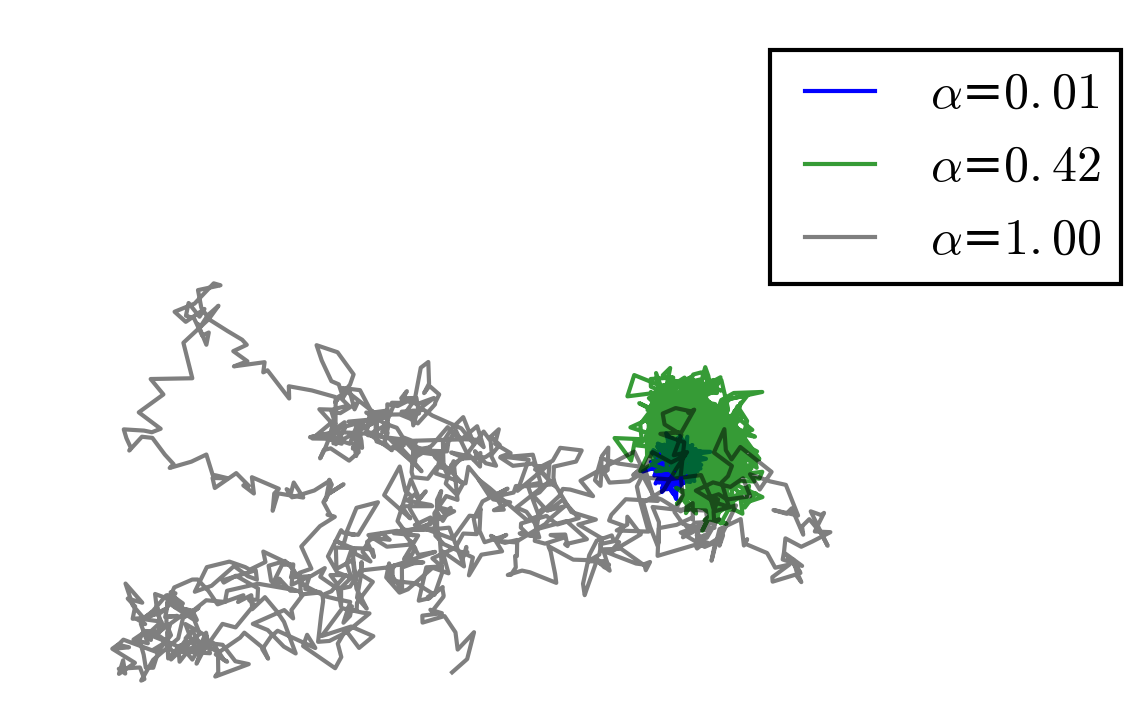
\includegraphics[width=0.7\textwidth]{./data/trajectories_differentalpha1234.png}
\caption{A three dimensional fBm trajectories for the anomalous coefficient $0.01\leq\alpha\leq 1$ generated with the Lowen algorithm are shown. The general diffusion constant, the time step and trajectory length were chosen as follows:  $K_{\alpha}=1$, $\Delta t=1$, $M=1000$.}
\label{alphachangetrajectory}
\end{figure}
In the previous section the MSD has been shown to be linear with time as a result of the central limit theorem. In normal liquids this behavior can be seen already at time scales higher than picoseconds \cite{Hofling2013}. Nevertheless, many experiments show that the MSD has a power law behavior ( $\delta r ^2 (t) \propto t^{\alpha}$ for  $0 < \alpha < 1$ ) over certain time windows form  microseconds to even seconds. Thus, the central limit theorem does not hold, at least in theses time scales. It can be shown that persistent correlations of the increments are present. In soft matter, like polymers, a sub-diffusive behavior is typically present in a time window but finally the linear MSD takes over. Fractional Brownian motion idealizes this situation by imposing that the central limit theorem is violated even for all time scales. The basic feature of fBm's is that the "span of interdependence" between their increments can be said to be infinite \cite{Mandelbrot1968} \par
Just like the Wiener process, continuous-time Fractional Brownian motion (ctfBm) is a continuous-time Gaussian process $\{B^{\alpha}_t\}: \Omega \rightarrow \mathbb{R}^d$ at time $t \in T$ in the observation time $T =[0, \infty)$. It is fully specified by its mean $\langle B_t \rangle=0$ and its covariance function:
\begin{align}
\mathrm{Cov}[B^{\alpha}_t,B^{\alpha}_s]=\frac{\sigma^2}{2}[t^{\alpha}-2(s-t)^{\alpha}+s^{\alpha}] \qquad \text{for} \qquad t<s \label{correlationfunctionfbm}
\end{align}
With the mean and the covariance defined, the mean square displacement for fBm can be derived as: 
\begin{align}
\label{MSDfbm}
 \langle (B^{\alpha}_{t}-B^{\alpha}_{s})^2 \rangle = (s-t)^\alpha \sigma^2
\end{align}
Fractional Brownian motion exhibits a power law behavior of the mean square displacement and therefore indeed motivates to act as a model for anomalous diffusion.\par Fractional Brownian motion can be alternatively expressed in terms of its incremental sequence. The incremental sequence is a related stochastic process called continuous-time fractional Gaussian noise (ctfGn). CtfGn is a continuous-time Gaussian process $\{X^{\alpha}_t\}: \Omega \rightarrow \mathbb{R}^d$ at time $t \in T$ in the observation time $T =[0, \infty)$. The mean is zero  $\langle X^{\alpha}_t \rangle=0$   and variance $\mathrm{Var}[X^{\alpha}_t]= \langle (X^{\alpha}_t)^2 \rangle=\sigma^2$:
\begin{align}
  B^{\alpha}_t=\int^t_s X^{\alpha}_{t'} d t' +  B^{\alpha}_s \qquad \text{for} \qquad t<s
\end{align}
The covariance function for ctfGn can be derived from the covariance function of fractional Brownian motion:
\begin{align}
\mathrm{Cov}[X^{\alpha}_t,X^{\alpha}_s]&= \frac{d^2}{dt ds} \mathrm{Cov}[B^{\alpha}_t B^{\alpha}_s]=\sigma^2 \frac{d^2 |t-s|^{\alpha}}{dtds} \label{eq:covfgn} \\
 &=\alpha (\alpha-1) \sigma^2 |t-s|^{\alpha-2}+\alpha \sigma^2 |t-s|^{\alpha-1} \delta(t-s) \label{eq:covfgn1}
\end{align}
The first term of this covariance function is describing the correlation of the increments. For Wiener white noise ($\alpha=1$) the first terms disappears:
\begin{align}
 \mathrm{Cov}[X_t,X_s]= \sigma^2 \delta(t-s)
\end{align}
The description of fractional Brownian motion in terms of fractional Gaussian noise is often convenient because of fGn's stationarity. It is possible to apply the Wiener-Khinchin theorem on a stationary random process. Thus, a spectral decomposition exists. The power spectral density can be written as the Fourier transform of the auto-covariance function:
\begin{align}
 S(\omega)= \int^{\infty}_{-\infty} \mathrm{Cov}[X_t,X_0] \exp[-2 \pi i \omega t] dt
\end{align}
The power spectral density for fGn for $\omega \longrightarrow 0$ can be written as \cite{Hofling2013}:
\begin{align}
 S(\omega)_{fGn}= \sigma^2 \Gamma(1+\alpha) (-i \omega)^{1-\alpha} \label{powerspec}
\end{align}
For the Wiener white noise ($\alpha=1$) the result simplifies to a constant:
\begin{align}
 S(\omega)_{Gn} = \sigma^2 
\end{align}
For fBm generating algorithms the discrete time version of fractional Brownian motion (fBm) and Gaussian noise (fGn) are interesting as well. The relation between them can be written as:
\begin{align}
B^{\alpha}_{t}= \sum_{i=0}^kX^{\alpha}_{t_i} \qquad \text{with} \qquad t_i= t_0+i \Delta t
\end{align}
The covariance function of discrete time fractional Gaussian noise is:
\begin{align}
 \mathrm{Cov}[X^{\alpha}_n,X^{\alpha}_m]&=\langle (B^{\alpha}_{n+1}-B^{\alpha}_n) (B^{\alpha}_{m+1}-B^{\alpha}_m)\rangle \\ &=\frac{\Delta t^{\alpha} \sigma^2}{2}[(n-m-1)^{\alpha}-2(n-m)^{\alpha}+(n-m+1)^{\alpha}]\\ &  \text{for}  \quad n\geq m
\end{align}
Due to stationarity one can write the auto-covariance function as:
\begin{align}
 \mathrm{Cov}[X^{\alpha}_0,X^{\alpha}_n]=\frac{\Delta t^{\alpha}\sigma^2}{2}[(n-1)^{\alpha}-2n^{\alpha}+(n+1)^{\alpha}] \label{autocovfgn}
\end{align}
A more detailed study of fBm and fGm can be found in \cite{qian2003fractional}.\par \bigskip Similar to the line of argument for Brownian motion, also fBm needs a connection to the strength of diffusion. This connection is introduced by the variance of fGn as: 
\begin{align}
\label{diffusionvariance}
\sigma^2=2dK_{\alpha} 
\end{align}
The mean square displacement for fBm follows from \cref{MSDfbm} as:
\begin{align}
\delta r^{2}(t)=2dK_{\alpha} t^{\alpha}
\end{align}
Here  $K_{\alpha}>0$  is the generalized diffusion coefficient of the physical dimension $ \mathrm{cm^2/sec^{\alpha}} $. The more physical description in terms of a propagator is the correlation function of the single particle density $P(\bm{r}-\bm{r}',t-t')= V\langle\rho(\bm{r},t) \rho(\bm{r}',t')\rangle$. Here, the single particle density $\rho(\bm{r},t)=\langle \delta(\bm{r}-\bm{R}(t))\rangle$ describes the density of a particle, which is localized at position $\bm{R}(t)$. $V$ is the volume. Just like Brownian motion, fractional Brownian motions increments $\Delta \bm{R}$ are Gaussian distributed with zero mean. The single particle density results in:
\begin{align}
 P(\bm{r},t)=[4 \pi K_{\alpha} t^{\alpha}]^{-d/2} \exp \left[ \frac{-|\bm{r}|^2}{ 4 K_{\alpha} t^{\alpha} }\right]
\end{align}
The propagator of fBm can be transformed into a scale free form. A scale free form will be we relevant in the analysis of the algorithm. It is related to the scale free form of standard Brownian motion \cref{scalefreeform}:
\begin{align}
P(\bm{r},t)&= \bm{r}^{-d} \mathcal{P}_{gauss}(\hat{\bm{r}}) \\ \text{with} \qquad \hat{\bm{r}} &= \frac{\bm{r}}{\sqrt{2 K_{\alpha} t^{\alpha}}}  \quad \text{and} \qquad \mathcal{P}_{gauss}(\bm{\hat{r}})= (2 \pi)^{-d/2}  \bm{\hat{r}}^d \exp \left(- \frac{|\bm{\hat{r}}|^2}{2} \right)\label{scalefreeformfrac}
\end{align}
Velocities ($\bm{\xi}(t)$) in the physical world can be described by fractional Brownian noise. The velocity auto-correlation function (VACF) ($Z(t)$) can be expressed from the auto-covariance function of fGn as defined in \cref{eq:covfgn}:
\begin{align}
Z(|t-t'|)&= \frac{1}{d}\langle \bm{\xi}(t) \bullet \bm{\xi}(t') \rangle = \frac{1}{2d} \frac{d^2}{dt^2} \delta r^2 (t-t')  
\end{align}
The frequency representation of the velocity auto-correlation function of fractional Brownian motion is defined analogously to \cref{powerspec} as:
\begin{align}
  \tilde{Z}(\omega) =  K_{\alpha} \Gamma(1+\alpha)(i \omega)^{1-\alpha}
\end{align}
\begin{comment}
\item The van hove correlation function can be transformed via the spatial Fourier transform into its wave-number representation, which is called the self-intermediate scattering function. Again for isotropic systems one can write $|\bm{k}|=k$.
\begin{align}
 F_{s}(k,t)&=\langle\rho(k,t) \rho(k',t')\rangle=\int d^{d}r e^{-i k r} P(r,t) \\
 &=\langle e^{-i k \Delta R(t)} \rangle
\end{align}
\item 
\end{comment}
For the analysis of fBm generating algorithms an indicator, if the created increments indeed are Gaussian, will be of interesting. One can show that for Gaussian propagators with zero-mean all but the second cumulants vanish. For non-Gaussian transport also further cumulants are non-zero. The cumulants can be obtained by expanding the characteristic function of $\Delta R(t)$ for small wave numbers $k \rightarrow 0$. Its logarithm returns the cumulants. From the cumulants the so called non-Gaussian parameter can be defined \cite{Hofling2013}:
\begin{align}
 \alpha_2=\frac{d \delta r^{4}(t)}{(d+2) [\delta r^{2}(t)]}-1 \label{nongaussian2}
\end{align}
The non-Gaussian parameter shows non-Gaussian transport if $\alpha_2>0$. This in turn does not lead to sure Gaussian transport for $\alpha_2>0$. Cumulants of higher order still can be non-zero. 
\begin{comment}
An other important quantity is the dynamical structure factor, which is the time-frequency Fourier transform of the intermediate scattering function:
\begin{align}
 F_{s}(k,z)&=\langle\rho(k,z) \rho(k',z')\rangle=\int_{0}^{\infty} d t e^{-i t z} P(k,t) \text{ for } k \rightarrow 0 , \operatorname{Im}(z) > 0 \label{dynamicstructurfactor}\\
 &= \frac{1}{-iz}-\frac{k^2}{2d}\int_{0}^{\infty} d t e^{izt} \delta r^2 (t) + \mathcal{O}(k^2)
\end{align}
For the velocities as our random variables $\partial_t \bm{R}(t)=\bm{\xi}(t)$ also the Velocity auto correlation function is of interest. Velocities correspond to continuous-time fractional Gaussian noise in the mathematical description. 

\begin{itemize} 
\item Velocities can be used to calculated the Velocity Autocorrelation Function (VACF):
\begin{align}
Z(|t-t'|)&= \frac{1}{d}\langle \bm{\xi}(t) \bm{\xi}(t') \rangle = \frac{1}{2d} \frac{d^2}{dt^2} \delta r^2 (t-t')  
\end{align}
The VACF in the frequency domain for fBm is: 
\begin{align}
  \tilde{Z}(z) \stackrel{\operatorname{Im}(z)> 0} {=}  K_{\alpha} \Gamma(1+\alpha)(i z)^{1-\alpha}
\end{align}
The calculation can be found in the appendix \ref{VACF}
\end{itemize}
\end{comment}

\section{Algorithm}
Effects of anomalous diffusion increase their relevance for long time. Thus, a fractional Brownian motion generating algorithm for preferably long trajectories is going to be searched for. Exactness and performance of the algorithm matter. In literature several algorithms are described. Promising exact methods are: Cholesky \cite{Dieker2004}, Hosking \cite{WRCR:WRCR3676}, Davis-Harte \cite{Dieker2004} and  Lowen \cite{Lowen1999} method. Cholesky  method claim to perform $\mathcal{O}(M^3)$ in respect to the length of trajectory $M$ and $\mathcal{O}(M^2)$ for every next trajectory. Davis-Harte and Lowen method claim to be exact and fast $\mathcal{O}(M log(M))$ \cite{DAVIES1987}\cite{Lowen1999}. There are further algorithms with even faster performance (e.g. the $RMD_{3,3}$- method \cite{Dieker2004} with $\mathcal{O}(M)$) . However, they are approximations. In order to choose an algorithm, four algorithms were analyzed in terms of accuracy and speed. 1.Cholesky  2. Davis-Harte 3.Lowen and 4. an own naive algorithm. All the methods are based on one or the other correlation functions described in the previous section.  
\subsubsection{Cholesky Method}
\begin{table}
\begin{framed}
\begin{enumerate}
 \item Calculate the covariance matrix of fGn:
 \begin{align}
  \Gamma=(\mathrm{Cov[x_i,x_j]}) \quad , \\  \mathrm{Cov[x_i,x_j]}=\Delta t^\alpha \sigma^2(i^{\alpha}+j^{\alpha}-|i-j|^\alpha)/2
 \end{align}
\item Calculate the eigenvalues $\lambda$ and eigenvectors $\bm{v}$ of $\Gamma$ 
\item Compute $\Sigma$ the square root of $\Gamma$ by the eigenvalues.
\item Draw for every entrance of the vector $\bm{\eta}$  a standard Gaussian distributed random number. Length of the vector is defined by the length $M$ of the trajectory:
\begin{align}
 \eta_k= \mathcal{N}(0,1) \quad \text{,}  \qquad k=0,1,2,...,M 
\end{align}
\item Calculate the fGn by $B^{\alpha}_k =\Sigma \bm{\eta_k}$.
\end{enumerate}
\end{framed}
\caption{The table shows Choleskys method to generate fBm.}
\label{Choleskimethod}
\end{table}
The Cholesky method \cite{Dieker2004} is based on the auto-covariance function of fGn as described by \cref{correlationfunctionfbm}. The algorithm is shown in \cref{Choleskimethod}. This approach is simple but as claimed by \citet{Dieker2004} unfortunately not efficient in respect to the trajectory length ($\mathcal{O}(M^3)$). Performance and accuracy of all algorithms are discussed in detail in the last two sections of the chapter.
\subsubsection{A Naive Algorithms}
\begin{table}
\begin{framed}
\begin{enumerate}
 \item Generate $4M$ independent normally distributed random increments: 
\begin{align}
 \eta_k \sim \mathcal{N}(0,\sqrt{\Delta t})\quad, \qquad k=0,1,2,...,4M 
\end{align}
\item Fourier transform the increments via FFT into the frequency domain:
\begin{align}
 \tilde{\eta_l}=\sum_{k=0}^{4M-1} \eta_k \exp\left[\frac{- i 2 \pi  l k }{4M}\right] \Delta t \quad , \qquad  l=0,1,2,...,4M  \label{eq:fouriertrans}
\end{align}
\begin{comment}
By comparison with the \cref{eq:fourier} one can see that:
\begin{align}
 z \rightarrow  l \Delta z \text{ , } \Delta z =   \frac{2 \pi }{M \Delta t} \text{ , } t \rightarrow j \Delta t \text{ and } \int dt \rightarrow \sum \Delta t \label{eq:diskret-freq} 
\end{align}
 \end{comment}
\item Generated fractional increments in the frequency domain with the VACF: 
 \begin{align}
   \tilde{\xi}_{l}&= \tilde{\eta}_l\sqrt{2 Re( \tilde{Z}_l)} \label{eq:problem} 
  \end{align}
 Here,  $ \tilde{Z}_l$ is the discrete VACF in the frequency domain:
  \begin{align}
   \tilde{Z}_l = K_{\alpha} \Gamma(1+\alpha)(i 2 \pi l \Delta \omega)^{1-\alpha} =  K_{\alpha} \Gamma(1+\alpha)\left( \frac{i l 2 \pi}{4 M \Delta t}\right)^{1-\alpha} 
 \end{align}
 
 \item Replace the zero-increment in the frequency domain with:
\begin{align}
 \tilde{\xi}_{l=o} = \mathcal{N}(0,\sqrt{2 K_{\alpha} (4 M \Delta t)^\alpha})
\end{align}
 \item Reverse Fourier transform the increments into the time domain:
 \begin{align}
 \xi_{k}= \frac{1}{4M} \sum_{l=0}^{4M-1}  \tilde{\xi}_l \exp\left[\frac{2 \pi i l k }{4M}\right] \Delta \omega
 \end{align}
 \item Build the cumulative sum only for the first quarter of the total number of generated increments: 
 \begin{align}
   B^{\alpha}_n= \sum^{n-1}_{k=0} \xi_k ,\qquad n=(0,1,..,M)
  \end{align}
\end{enumerate}
\end{framed}
\caption{The table shows a naive algorithm to generate fBm.}
\label{naivealgorithm}
 \end{table}
\begin{figure}[h]
  \centering
  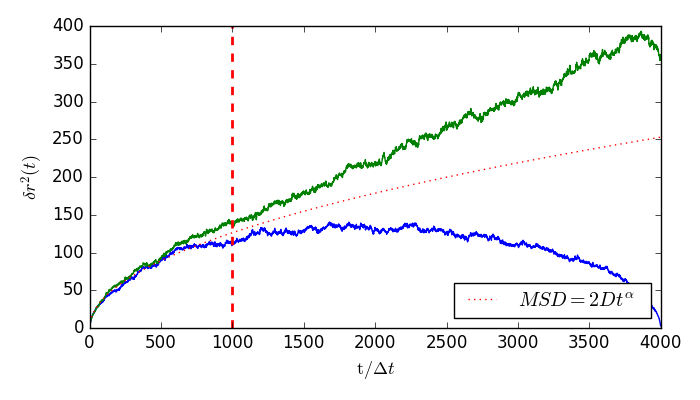
\includegraphics[width=\textwidth]{./data/boundary_problem.png}
  \captionsetup{width=\linewidth}
  \captionof{figure}{An ensemble average mean square displacement of two versions of the naive algorithm. The green curve is the MSD of the algorithm with the correction introduced in step 4 and the blue curve without.}
  \label{fig:41}
\end{figure}
In this section a naive algorithm based on the VACF in the frequency domain is introduced. This was the first attempt of a fast fBm algorithm, without any insight from the existing literature. The idea is to compute the increments in the frequency domain and eventually transform them back to the time domain. The algorithm is described in \cref{naivealgorithm}. In the first step of the algorithm four times the amount of increments in comparison to the trajectory length are generated. It counteracts a problem arising from the boundary problem of the FFT. The problem is visualized in \cref{fig:41}. The figure shows an ensemble-averaged mean square displacement for $\alpha=0.5$ for two versions of the algorithm. The blue curve is the curve without any modification and the green curve  for the algorithm with the modification introduced in step 4. The blue curve is for now of interest. It can be seen that on average all the particles travel back to their initial position. It is not shown in the plot, however this is even true for every trajectory. The FFT has a downside compared to the continuous Fourier transform, which causes this effect. The VACF is zero at zero-frequency $ \tilde{Z}_{l=0}=0$.  From \cref{eq:problem} also the first increment in the frequency domain is zero $ \tilde{\xi}_{l=0}=0$. Due to \cref{eq:fouriertrans} also the following relation holds:
 \begin{align}
   \tilde{\xi}_{l=0} = \sum_{k=0}^{M-1} \xi_k e^{0} \Delta t = \Delta  R_{M} \label{correction}
 \end{align}
$\Delta R $ is the distance between the starting point and the position of the particle. Therefore, the particle would travel after $M$ steps back to its initial position. The naive idea is to generate a trajectory four times longer than the desired length and only take the first forth into consideration. This can be thought of as a finite-time correction. The cut is displayed as a vertical red dashed line. The plot suggests not a perfect but at least a better agreement of the generated data to the theoretical mean square displacement displayed as a dotted line for short times. Hereafter the normally distributed random numbers are transformed into the frequency domain to apply Wiener-Khinchin's theorem by multiplying with the square root of two times VACF. Besides taking only one quarter of the trajectory a modification to the algorithm was introduced in step 4. Its impact in the MSD is shown in \cref{fig:41} as the green line. Instead accepting  \cref{correction}, the zero-frequency increment is calculated as follows:
\begin{align}
 \tilde{\xi}_{l=0} = \mathcal{N}(0,\sqrt{2 K_{\alpha} (M \Delta t)^\alpha})
\end{align}
This equation would be correct if we assumed fractional Brownian motion to be a Markovian process. This is certainly is not the cause. This approximation seems to improve the accuracy only slightly.
Finally in step 4 the increments are back transformed into the time domain and in step 5 the cumulative sum of fGn is calculated, which yields fBm. The described algorithm can be performed independently for every Cartesian component of the three dimensional fractional Brownian motion. Different Cartesian components are independent. Without any extensive analysis of the naive algorithm one can already conclude draw backs in terms of convergence close to the overall simulation time. 
\begin{comment}
in step 4: The discrete Fourier transform has a downside compared to the continuous Fourier transform, as already noted in the beginning of this section. The VACF is zero at zero-frequency $ \tilde{Z}_{l=0}(z=0)=0$.  From \cref{eq:problem} also the first increment in the frequency domain is zero $ \tilde{\xi}_{l=o}(z=0)= 0$. Due to \cref{eq:fouriertrans} also the following relation holds:
 \begin{align}
   \tilde{\xi}_{l=o}(z) = \sum_{k=0}^{M-1} \xi_k e^{0} \Delta t = \Delta  R_{M} \label{correction}
 \end{align}
$\Delta R $ is the distance between the starting point and the position of the particle. Therefore, the particle would travel after $M$ steps back to its initial position. The effect on the ensemble averaged mean square displacement can be seen in \cref{fig:6}. 

will be used to modify standard Brownian motion velocities, which are easily computable, to generate increments. The starting point are the velocities $\partial_t \bm{R}(t)=\bm{\xi}(t)$. The increments can be decomposed in its Fourier modes for real frequencies $z=\omega$:
\begin{align}
 \tilde{\bm{\xi}}_{T}(\omega)=\int_{-\frac{T}{2}}^{\frac{T}{2}} dt e^{i \omega t} \bm{\xi}(t) \label{eq:fourier}
\end{align}
For a finite observation time T the Wiener-Khinchin theorem applies :
\begin{align}
 \lim_{T\to\infty}\frac{1}{T}\langle \lvert  \tilde{\bm{\xi}}_{T}(\omega) \rvert^2  \rangle = 2  \operatorname{Re} \left(\tilde{Z}(\omega)\right)
\end{align}
For white noise one gets: 
\begin{align}
 \lim_{T\to\infty}\frac{1}{T}\langle \lvert  \tilde{\bm{\eta}}_{T}(\omega) \rvert^2 \rangle = const.
\end{align}
Fractional correlations can be incorporated via its VACF:
\begin{align}
\tilde{\bm{\xi}}(\omega) = \sqrt{2 \operatorname{Re} \left(\tilde{Z(\omega)}\right)}  \tilde{\bm{\eta}}(\omega) \label{eq:fracvacf}
\end{align}
 With $\tilde{\bm{\xi}}(\omega)$ being fractional Brownian velocities in the frequency domain. Its Fourier-back-transform results in fractional Brownian velocities in the time domain.
\begin{align}
\bm{\xi}(t)=\int d \omega e^{i \omega t} \tilde{\bm{\xi}}(\omega) \label{eq:fourier2}
\end{align}
In the following an algorithm, which generates fractional Brownian noise will be introduced. The algorithm is based on the Davis-Harte algorithm \cite{Craigmile2003}. The idea is to use the calculated VACF and thereby modify conventionally generated Gaussian random variables. All the increments should be generated beforehand. With this concept it is difficult to include forces. For computational reasons the previous elaborations on how to generate fractional Brownian increments have to be transformed into a discrete form, thereby the solution is no longer exact, which will be shown in the analysis part of the algorithm.  
\begin{align}
\bm{\eta} (t) \longrightarrow \bm{\eta}_j(t)  \text{  with  } j=0,1,2,...,n  \text{  ,  } n= \text{amount of steps}
\end{align}
For a n-steps long trajectory one can write:
\begin{align}
 \Delta \bm{R}_n(t) =  \sum_{j=0}^n \bm{\eta}_j  \Delta t \label{eq:diskretdeltar}
\end{align}
 The following algorithm is explained for one dimension and can be easily extended for more dimensions. The MSD can be written as:
\begin{align}
< \Delta R_{j}(t)>=2K_{\alpha} (\Delta t j)^{\alpha}
\end{align}
The algorithm goes as follows:
\begin{enumerate}
 \item $M$ independent normally distributed random increments are generated: 
\begin{align}
 \eta_k(t)= \mathcal{N}(0,\sqrt{\Delta t}) \text{  with  } k=0,1,2,...,M 
\end{align}

$M>n$  more increments are generated to counteract the boundary problem in the discrete Fourier transform, which is shown in \cref{fig:6} and \cref{fig:5}

\item Via discrete Fourier transform these increments are transformed into the frequency domain:
\begin{align}
 \tilde{\eta_l}(z)=\sum_{k=0}^{M-1} \eta_k e^{\frac{- i 2 \pi  l k }{M}} \Delta t   \text{  with  }  l=0,1,2,...,M  \label{eq:fouriertrans}\\ 
\end{align}
By comparison with the \cref{eq:fourier} one can see that:
\begin{align}
 z \rightarrow  l \Delta z \text{ , } \Delta z =   \frac{2 \pi }{M \Delta t} \text{ , } t \rightarrow j \Delta t \text{ and } \int dt \rightarrow \sum \Delta t \label{eq:diskret-freq} 
\end{align}
 
\item Comparable to \cref{eq:fracvacf} correlations are incorporated: 
 \begin{align}
   \tilde{\xi}_{l}(z)&= \tilde{\eta}_l(z) \sqrt{2 Re( \tilde{Z}_l(z))} \label{eq:problem} 
  \end{align}
 with $\tilde{Z}(z)\rightarrow \tilde{Z}_l(z)$ as introduced in \cref{eq:diskret-freq}:
  \begin{align}
   \tilde{Z}_l(z) = K_{\alpha} \Gamma(1+\alpha)(i 2 \pi l \Delta z)^{1-\alpha} =  K_{\alpha} \Gamma(1+\alpha)(i l \frac{ 2 \pi}{M \Delta t})^{1-\alpha} 
 \end{align}
 
 \item The discrete Fourier transform has a downside compared to the continuous Fourier transform, as already noted in the beginning of this section. The VACF is zero at zero-frequency $ \tilde{Z}_{l=0}(z=0)=0$.  From \cref{eq:problem} also the first increment in the frequency domain is zero $ \tilde{\xi}_{l=o}(z=0)= 0$. Due to \cref{eq:fouriertrans} also the following relation holds:
 \begin{align}
   \tilde{\xi}_{l=o}(z) = \sum_{k=0}^{M-1} \xi_k e^{0} \Delta t = \Delta  R_{M} \label{correction}
 \end{align}
$\Delta R $ is the distance between the starting point and the position of the particle. Therefore, the particle would travel after $M$ steps back to its initial position. The effect on the ensemble averaged mean square displacement can be seen in \cref{fig:6}. Instead, the zero-increment in the frequency domain is calculated as follows:
\begin{align}
 \tilde{\xi}_{l=o} = \mathcal{N}(0,\sqrt{2 K_{\alpha} (M \Delta t)^\alpha})
\end{align}
\end{enumerate}




\begin{figure}
  \subfigure[Ensemble MSD without the correction introduced in \cref{correction}]{
  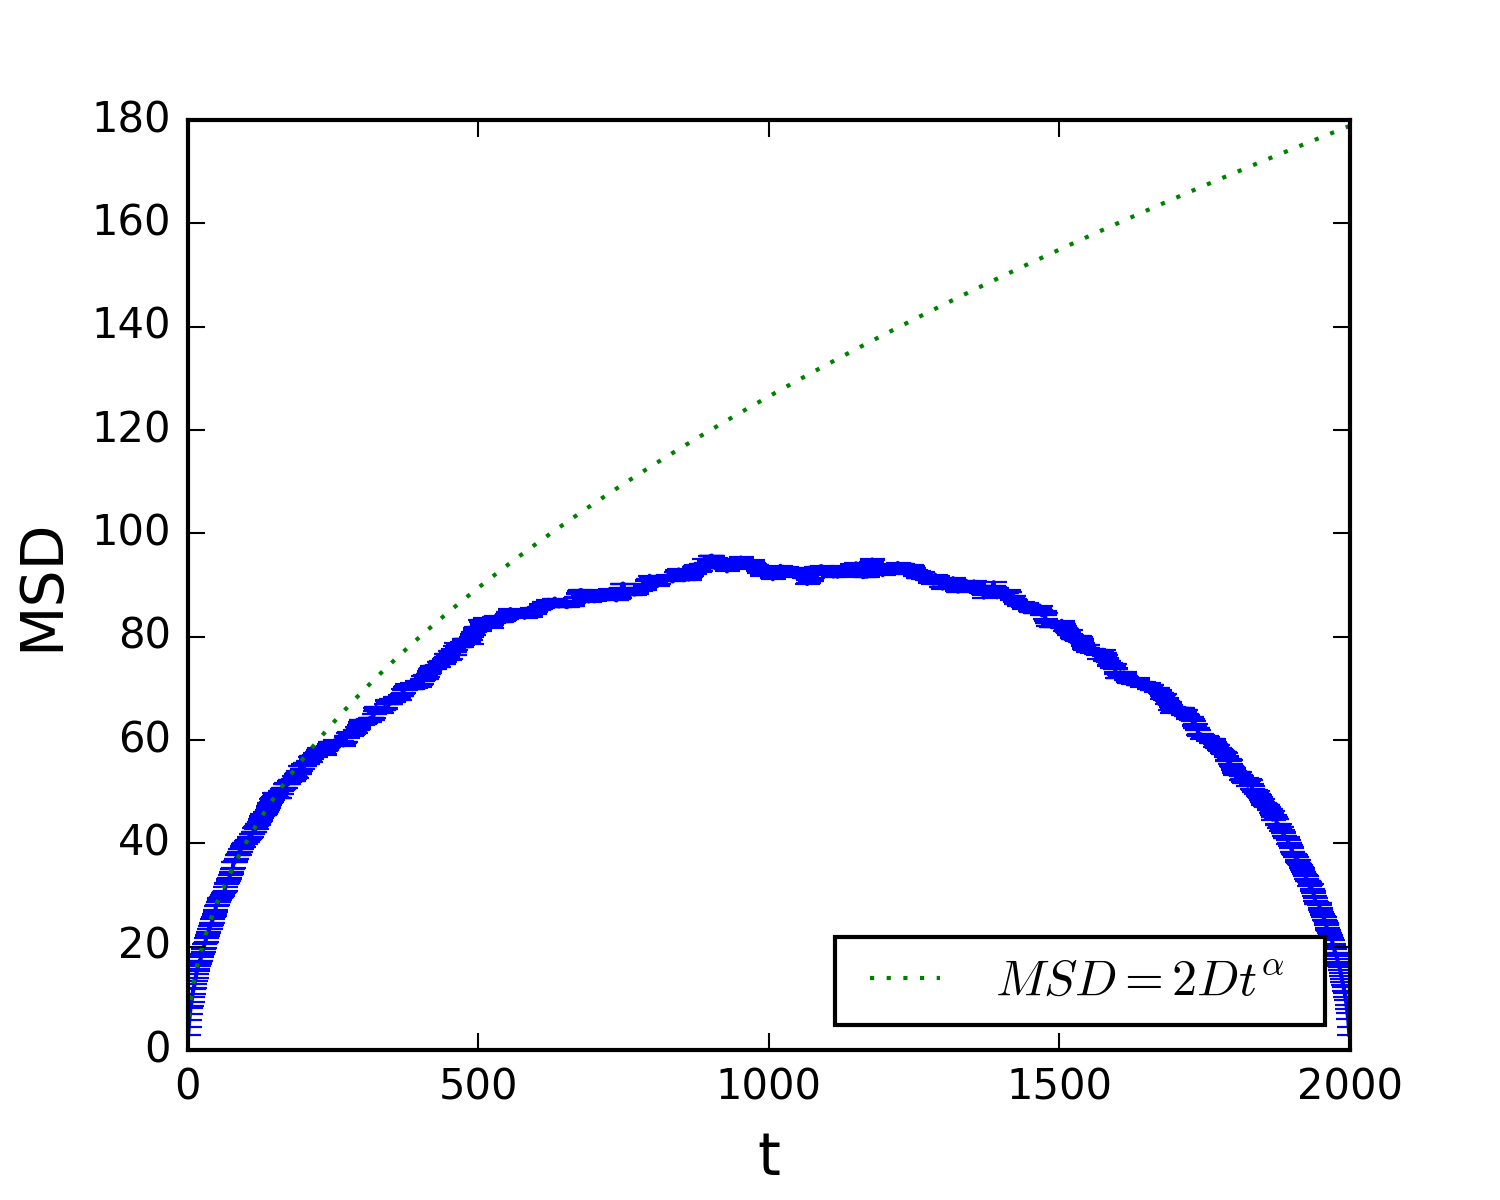
\includegraphics[width=0.5\textwidth]{./data/nocorrectionmsd.png}
  \label{fig:6}}
  \subfigure[Ensemble MSD with correction introduced in \cref{correction}. The side of the red bar indicates the threshold for the remaining increments for $M=2n$]{
  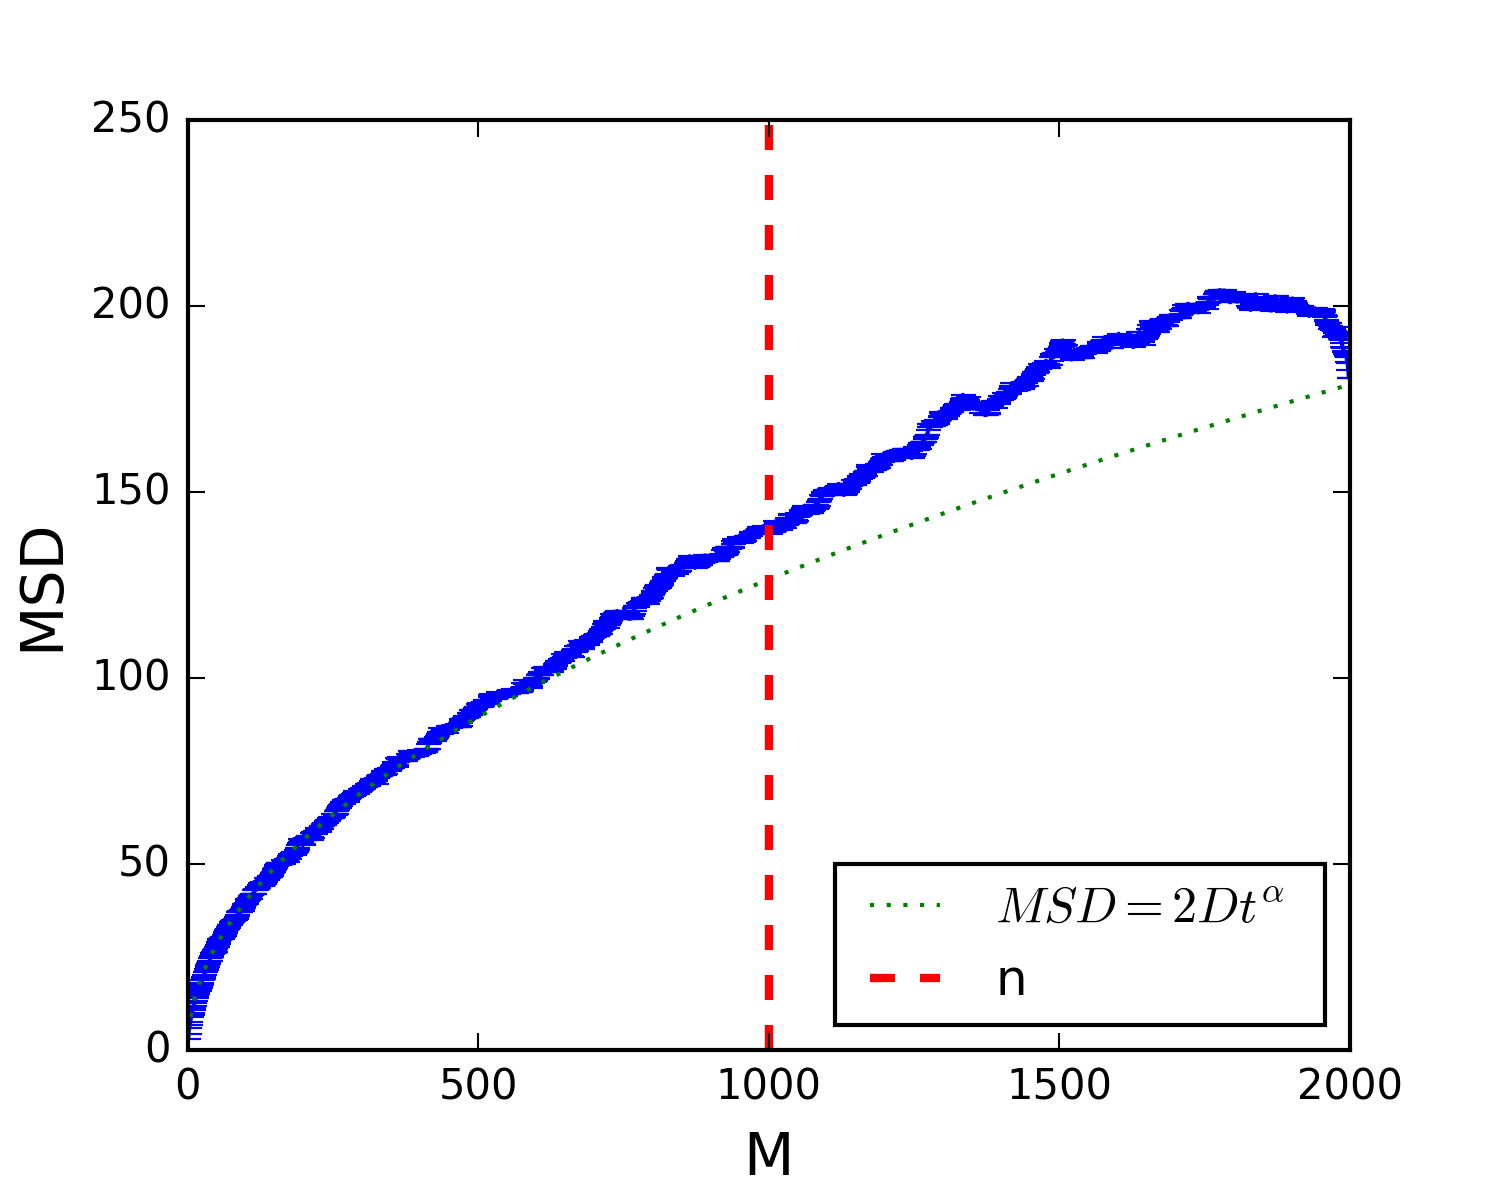
\includegraphics[width=0.5\textwidth]{./data/withcorrection_nocutoff.png}
  \label{fig:5}}
\end{figure}
This equation would be correct if we assumed fractional Brownian motion to be a Markovian process, which certainly is not the cause. This is also the reason why M have been chosen to be bigger than n. The presumption is, that the impact of the approximation would be negligible with increasing distance to $\Delta R_{M}$ and negligible at $\Delta R_{n}$. The impact on the ensemble averaged MSD can be seen in \cref{fig:5}. This can be thought of as a finite-time correction.

 %\item Laut dem Davies Harte Algorithmus wird außerdem das n-te Inkrement im Frequenzraum %umgeändert:
 %\begin{align}
 %\eta_{fbr_{g=n}} =\sqrt{Re(Z_g 2 n)} \mathcal{N}(0,1) 
 %\end{align}
 % Noch nicht verstanden warum!!
\end{comment}
\subsubsection{Lowen Algorithm}
\begin{table}[h]
 \begin{framed}
\begin{enumerate}
 \item Compute the auto-covariance function $R^{\xi}_n$ of a periodic stochastic process $\xi_n$:
 \begin{align}
  R^{\xi}_n=
  \begin{cases}
   \frac{1}{2}\left[1-\left(\frac{n}{N}\right)^{\alpha} \right]  & \text{ for    } 0 \leq n \leq M \\
   R^{\xi}_{2M-n}  & \text{ for    } M \leq n \leq 2M 
  \end{cases}
 \end{align}
 \item Transform the auto-covariance function via FFT. The result is called the spectral density of the stochastic process $\xi_n$:
  \begin{align}
   S^{\xi}_k= \mathrm{FFT}(R^{\xi}_n;k)
  \end{align}
 \item Calculate $\tilde\xi_k$ the Fourier transform of the stochastic process $\xi_n$:
 \begin{align}
  \tilde\xi_k=
  \begin{cases}
     0  & \text{ for    } k=0 \\    
     exp(i \theta_k) \eta_k \sqrt{S^{\xi}_k}  & \text{ for    } 0 \leq k \leq M \\
     \eta \sqrt{S^{\xi}_k}  & \text{ for    } k = M \\
     \tilde\xi^{*}_{2M-k} & \text{ for    } M \leq k \leq 2M 
  \end{cases}
 \end{align}
 $\{*\}$ denotes the complex conjugate, $\theta_k$ is a random phase uniformly distributed  in $(0,2\pi]$. $\eta_k$ is a random Gaussian variable with zero mean and variance 1 [$\eta_k\sim \mathcal{N}(0,1)$].  
 \item Perform the inverse Fourier transform on $\tilde\xi_k$ and use the first half of the resulting stochastic process $\xi_n$ multiplied by a factor:
 \begin{align}
  \xi_n&=\frac{\mathrm{FFT}^{-1}(\tilde\xi_k;n)}{2M} \\
  B^{\alpha}_n&=  \sqrt{2 K_{\alpha} M^{\alpha} \Delta t^{\alpha}} (\xi_n- \xi_0)  \qquad \qquad \text{for} \quad 0 \leq n \leq M
 \end{align}
\end{enumerate}
\end{framed}
\caption{The table shows Lowen's algorithm \cite{Lowen1999} to generate fBm.}
\label{Lowenalgorithm}
 \end{table}
 
 An algorithm by \citet{Lowen1999} was implemented. Lowens algorithm claims to be both fast $(\mathcal{O}(NlogN))$ and exact. However our implementation shows not to be exact, which is shown in the analysis part. It starts with a auto-covariance function $R^{\xi}_n$. Its second derivative yields the auto-covariance of discrete time fGn described by \cref{autocovfgn}. $R^{\xi}_n$ can be thought of as an auto-covariance function of a stationary periodic version of fBm. Lowens algorithm is described in \cref{Lowenalgorithm}. Lets check the resulting auto-covariance function of $B^{\alpha}_n$ resulting from the algorithm: 
\begin{align}
  & Cov[B^{\alpha}_n,B^{\alpha}_m]= 2 K_{\alpha} \Delta t^{\alpha} N^{\alpha} \langle (\xi_n- \xi_0) (\xi_m- \xi_0)\rangle \\
 &=  2 K_{\alpha} \Delta t^{\alpha} N^{\alpha}\langle\xi_n \xi_m\rangle -\langle \xi_0 \xi_m \rangle - \langle \xi_0 \xi_n\rangle +\langle \xi_0^2\rangle \\ 
 &= K_{\alpha} \Delta t^{\alpha}[n^{\alpha}-2(m-n)^{\alpha}+m^{\alpha}]\qquad \qquad \qquad \text{ for} \qquad n < m
\end{align}
The auto-covariance function indeed satisfies the condition for fBm with variance similar to \cref{diffusionvariance}. In step 3 the phase and amplitude of the Fourier transform  $\xi_m$ were chosen to be random  as suggested in \cite{Timmer1995}. The second derivative of $R_{\xi}(n) $ is positive. $R_{\xi}(n) $ results in a periodic function with non negative curvature. Its Fourier transform $S^{\xi}_k$ is , real, symmetric  and non-negative for all k. $S^{\xi}_k$ is then a valid power spectral density function of the discrete-time periodic process $\xi_n$ with period $2n$ and  $R^{\xi}_n$ its valid auto-covariance function \cite{Lowen1999}. This algorithm is actually using the property of Brownian scaling \cref{Brownianscaling} to generate a realization of fBm  with non negative auto-covariance function. 
\subsubsection{Davis-Harte Algorithm}
\begin{table}[h!]
 \begin{framed}
\begin{enumerate}
 \item Compute the auto-covariance function $R^{\xi}_n$ of a periodic stochastic process $\xi_n$:
 \begin{align}
  R^{\xi}_n= 
  \begin{cases}
    K_{\alpha} \Delta t^{\alpha}\left((n-1)^{\alpha}-2n^{\alpha}+(n+1)^{\alpha}\right) & \text{ for    } 0 \leq n \leq M \\
   R^{\xi}_{2M-n}  & \text{ for    } M \leq n \leq 2M 
  \end{cases}
 \end{align}
 \item Transform the auto-covariance function via FFT. The result is called the spectral density of the stochastic process $\xi_n$:
  \begin{align}
   S^{\xi}_k= \mathrm{FFT}(R^{\xi}_n;k)
  \end{align}
 \item Calculate $\tilde\xi_k$ the Fourier transform of the stochastic process $\xi_n$:
 \begin{align}
  \tilde\xi_k=
  \begin{cases}
     \sqrt{2 S^{\xi}_k M}(\eta_k) & \text{ for    } k=0 \\    
     \sqrt{ S^{\xi}_k M}(\eta_k+i \eta_k)  & \text{ for    } 0 \leq k \leq M \\
     \sqrt{2 S^{\xi}_k M}(\eta_k)  & \text{ for    } k = M \\
     \tilde\xi^{*}_{2M-k} & \text{ for    } M \leq k \leq 2M 
  \end{cases}
 \end{align}
 $\{*\}$ denotes the complex conjugate, $\eta_k$ is a random Gaussian variable with zero mean and variance 1 [$\eta_k\sim \mathcal{N}(0,1)$].  
 \item Perform the inverse Fourier transform on $\tilde\xi_k$ and use the first half of the resulting stochastic process $\xi_n$:
 \begin{align}
  \xi_n&=\frac{1}{\sqrt{2 M}} \mathrm{FFT}^{-1}(\tilde\xi_k;n) \qquad \text{for} \quad 0 \leq n \leq N
 \end{align}
 \item perform the cumulative sum on the incremetns:
 \begin{align}
  B^{\alpha}_n=\sum^n_{j=0} \xi_j \qquad \qquad \qquad \qquad \text{for} \quad 0 \leq n \leq M
 \end{align}
\end{enumerate}
\end{framed}
\caption{The table shows Davis-Harte algorithm \cite{DAVIES1987} to generate fBm.}
\label{Davies_harte-algorithm}
\end{table}
Davis-Harte algorithm \cite{DAVIES1987} is related Lowens Algorithm. It is also based on a FFT. The author claims the algorithm to be exact and its performance to scale with the length of the trajectory as $(\mathcal{O}(NlogN))$ . However, in contrast to Lowens algorithm it is based on the covariance function of fGn described by equation \cref{autocovfgn}. Thus it actually generates the increments of fBm. The  algorithm is shown in \cref{Davies_harte-algorithm}. 
\subsubsection{Accuracy Analysis}
The algorithms were implemented in Python and C++. For the C++ implementation a wrapper to Python was added. All algorithms were analysed by an analysis class. The C++ implementation is using the FFTW library for the Fast Fourier Transform \cite{FFTW} and Mersenne-Twister (gsl\texttt{\textunderscore}rng\texttt{\textunderscore}mt19937) \cite{Matsumoto1998} as the random number generator. Python implementations were developed beforehand and only serve as a reference. Python uses the numpy.fft library for the Fast Fourier Transform and also the Mersenne-Twister random number generator.\par
\begin{figure}[h!]
  \centering
  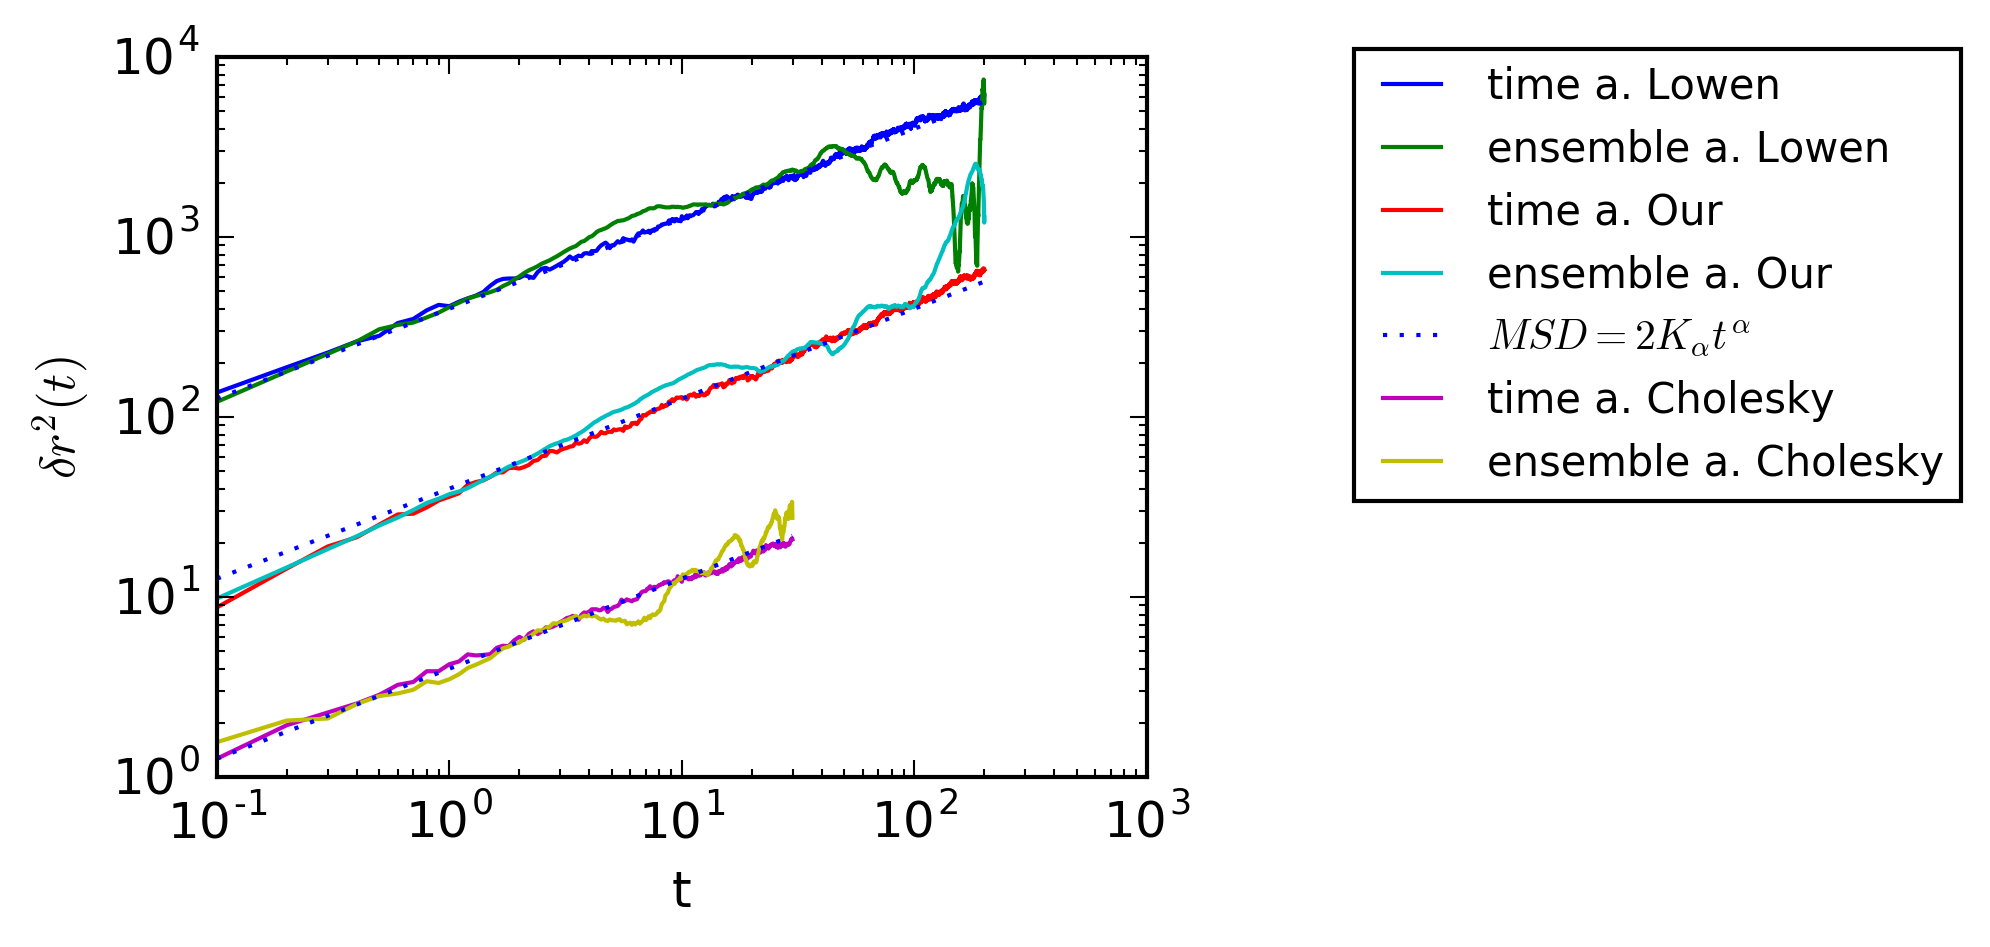
\includegraphics[width=\textwidth]{./data/timevsensambe.png}
  \captionsetup{width=\linewidth}
  \captionof{figure}{Comparison of MSD between time-average, ensemble-average ($N=1000$) ,$\alpha=0.5$, $\Delta t=0.1$ for the three algorithms.\newline Cholesky: $D=2$,  $M=300$.\newline Our $D=20$ $M=2000$, \newline  Lowen:  $D=200$ $M=2000$. }
  \label{fig:4}
\end{figure}
Insights of stochastic algorithms can be obtained by analyzing the observables. Observables of an stochastic process are generally averaged values. The motivation of choosing fBm was its power law behavior of the MSD. Therefore it is reasonable to analyze first this observable. It can be calculated as the ensemble- or time average. A difference in time and ensemble average would show a violation of ergodicity. A comparison for all four implemented algorithms can be seen in \cref{fig:4}. All algorithm show good accuracy between ensemble and time averaged MSD, besides for long lag times for the time averaged MSD due to decreasing statistics. Our algorithm tend to result in too  small MSDs for small lag times particularly for small $\alpha$, which is going be shown later on. This is caused by the finite amount of samples in the discrete Fourier transform. In the following figures all MSD plots are ensemble averages. They are computationally cheaper.\par Secondly time-reversibility had been checked. FBm should be time reversible as shown in \cite{Horvai2007}. In \cref{changeintime} MSDs for forward time and for backward time were plotted. No difference can be seen. $\alpha$ had been chosen to be $0.1$. Thereby our algorithm has an even stronger deviation from the desired power law.
\begin{figure}[h!]
\centering
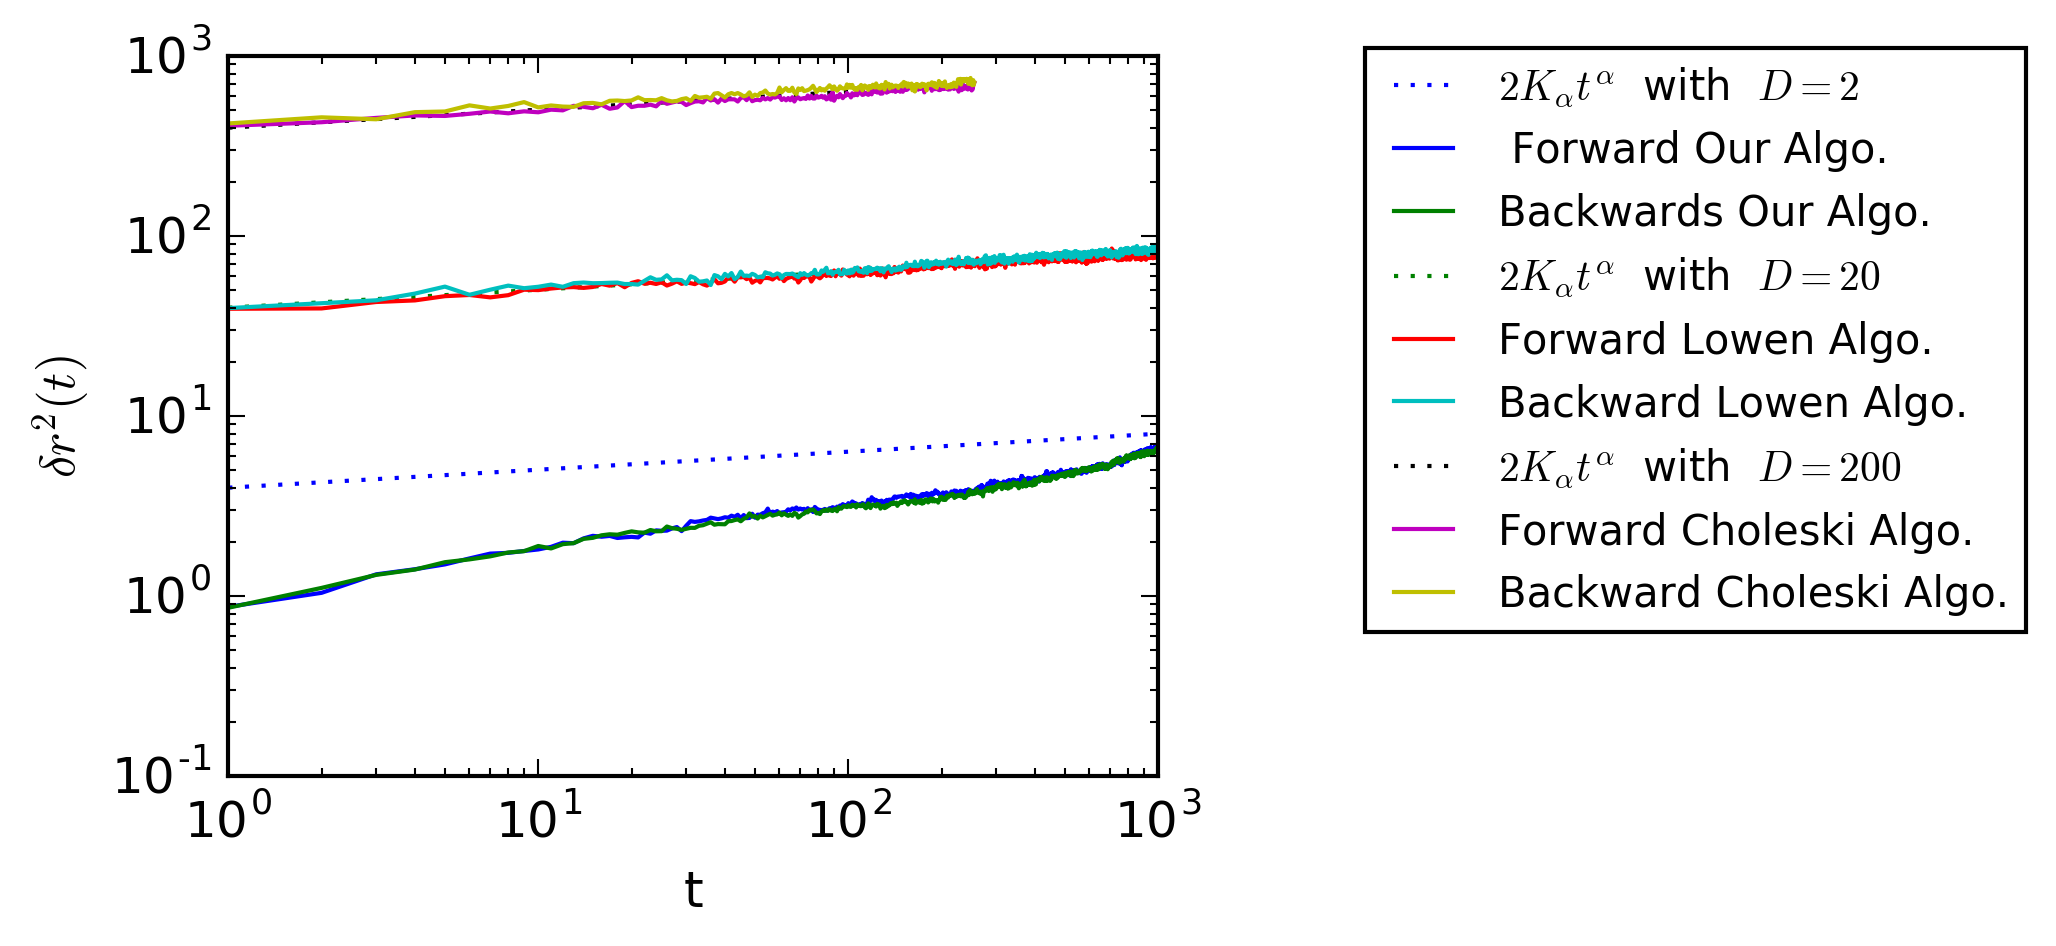
\includegraphics[width=\textwidth]{./data/changeintime.png}
\caption{The plot show ensemble averaged MSDs for forward time and backward time over $N=2000$ trajectories for $\alpha =0.1$, $\Delta t = 0.1$ and trajectory length $M=1000$ and $K_{\alpha}=2$ for Our algorithm, $M=1000$  $K_{\alpha}=20 $ for Lowen algorithm and  $M=256$  $K_{\alpha}=200$ for Cholesky algorithm.}
\label{changeintime}
\end{figure} 
A strong influence of $\alpha$ on the accuracy of MSD for our algorithm can be seen. The influence of $\alpha$ on the MSD for the three algorithms are shown in \cref{alphachange}. In the limit of Brownian motion $\alpha=1$ the artifacts for small lag-times in the our algorithm vanish. Cholesky and Lowen show no deviation to the expected MSD for all $\alpha$.
\begin{comment}
 


\newline \noindent The influence of the time step size is shown in \cref{fig:3} . The deviation from the expected value is linearly dependent on the amount of samples in the interval.
\begin{figure}[h!]
  \centering
  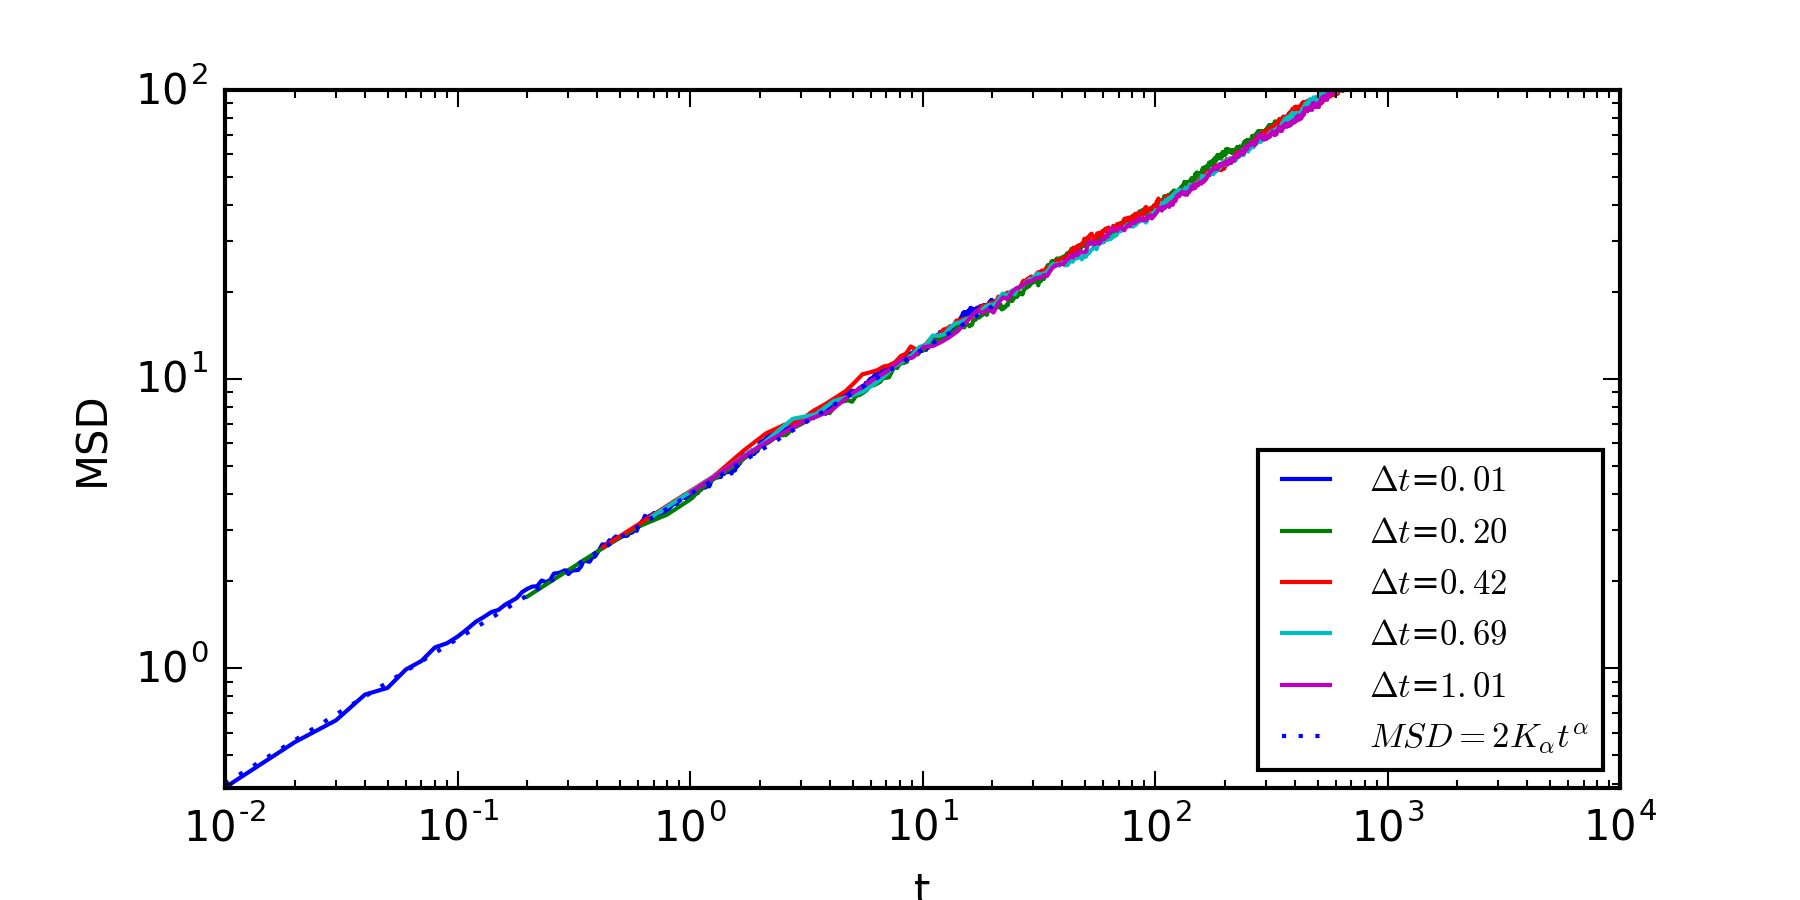
\includegraphics[width=\textwidth]{./data/dt_change.png}
  \captionsetup{width=\linewidth}
  \captionof{figure}{Comparison of ensemble averaged Mean-Square-Displacements with different $\Delta t$ for $D=2$, $\alpha=0.5$. }
  \label{fig:3}
\end{figure} 
\noindent 
\begin{figure}[h!]
\centering
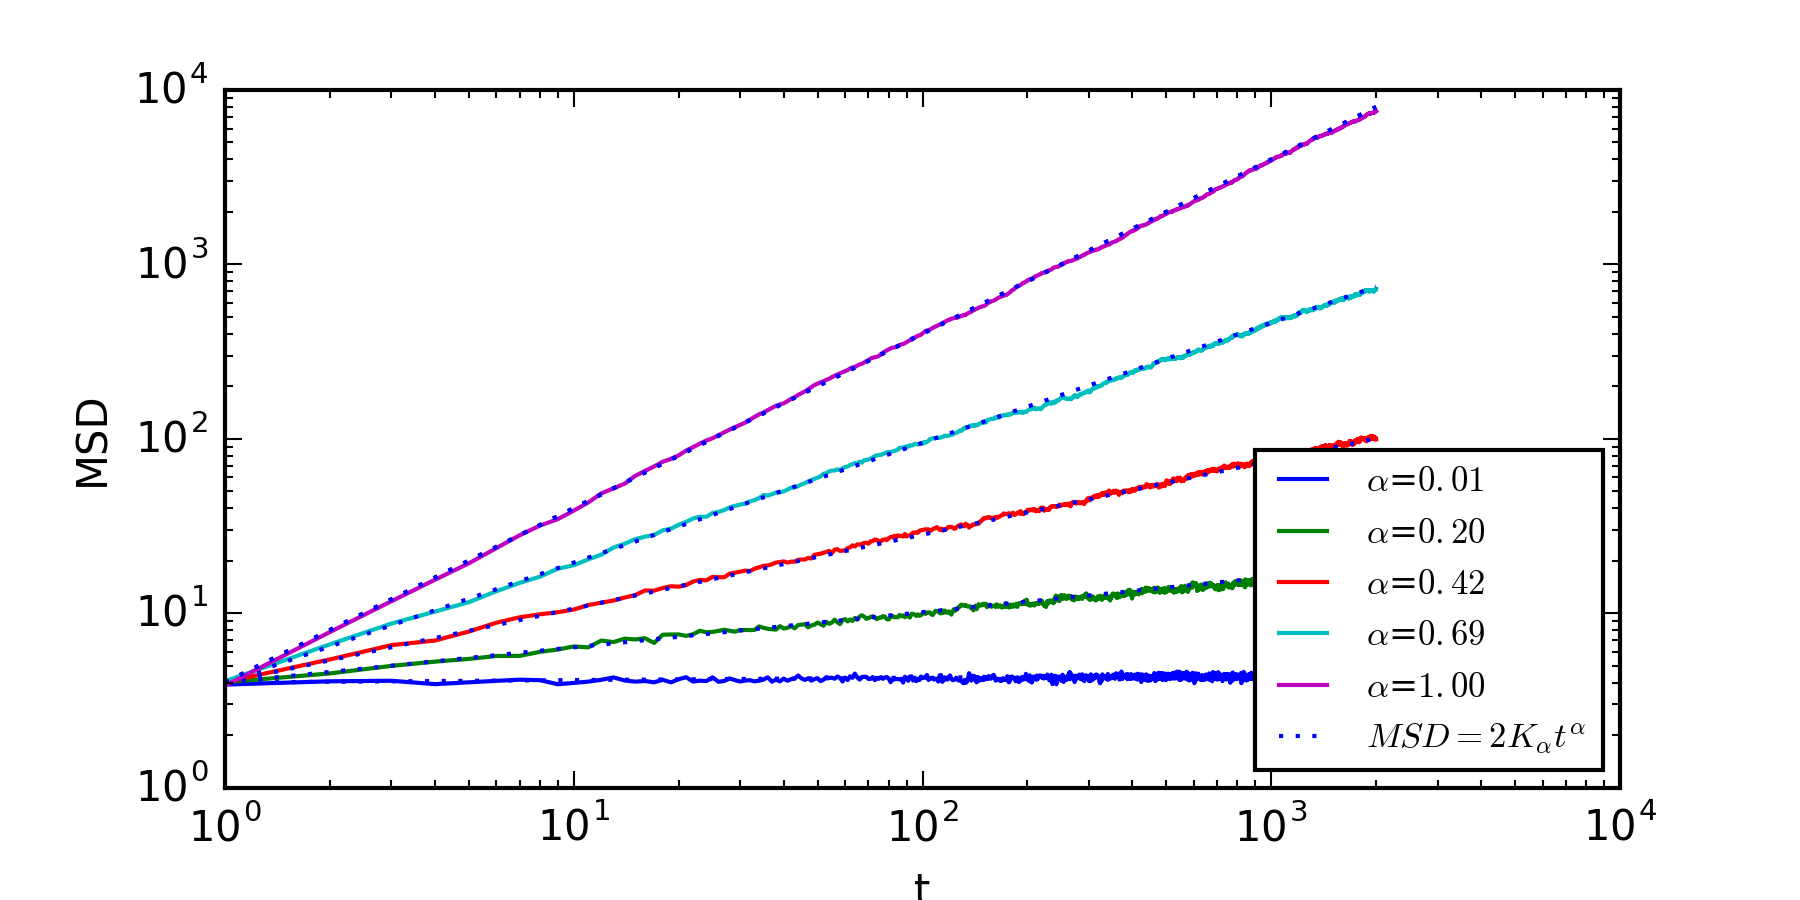
\includegraphics[width=\textwidth]{./data/alpha_change.png}
\caption{Ensemble averaged MSD for different $\alpha$  with $K_{\alpha}=2$ , $N=2000$, $n=2000$ , $\Delta t = 1$, $M=2n$.}
\label{alphachange}
\end{figure}
\begin{figure}[h!]
\centering
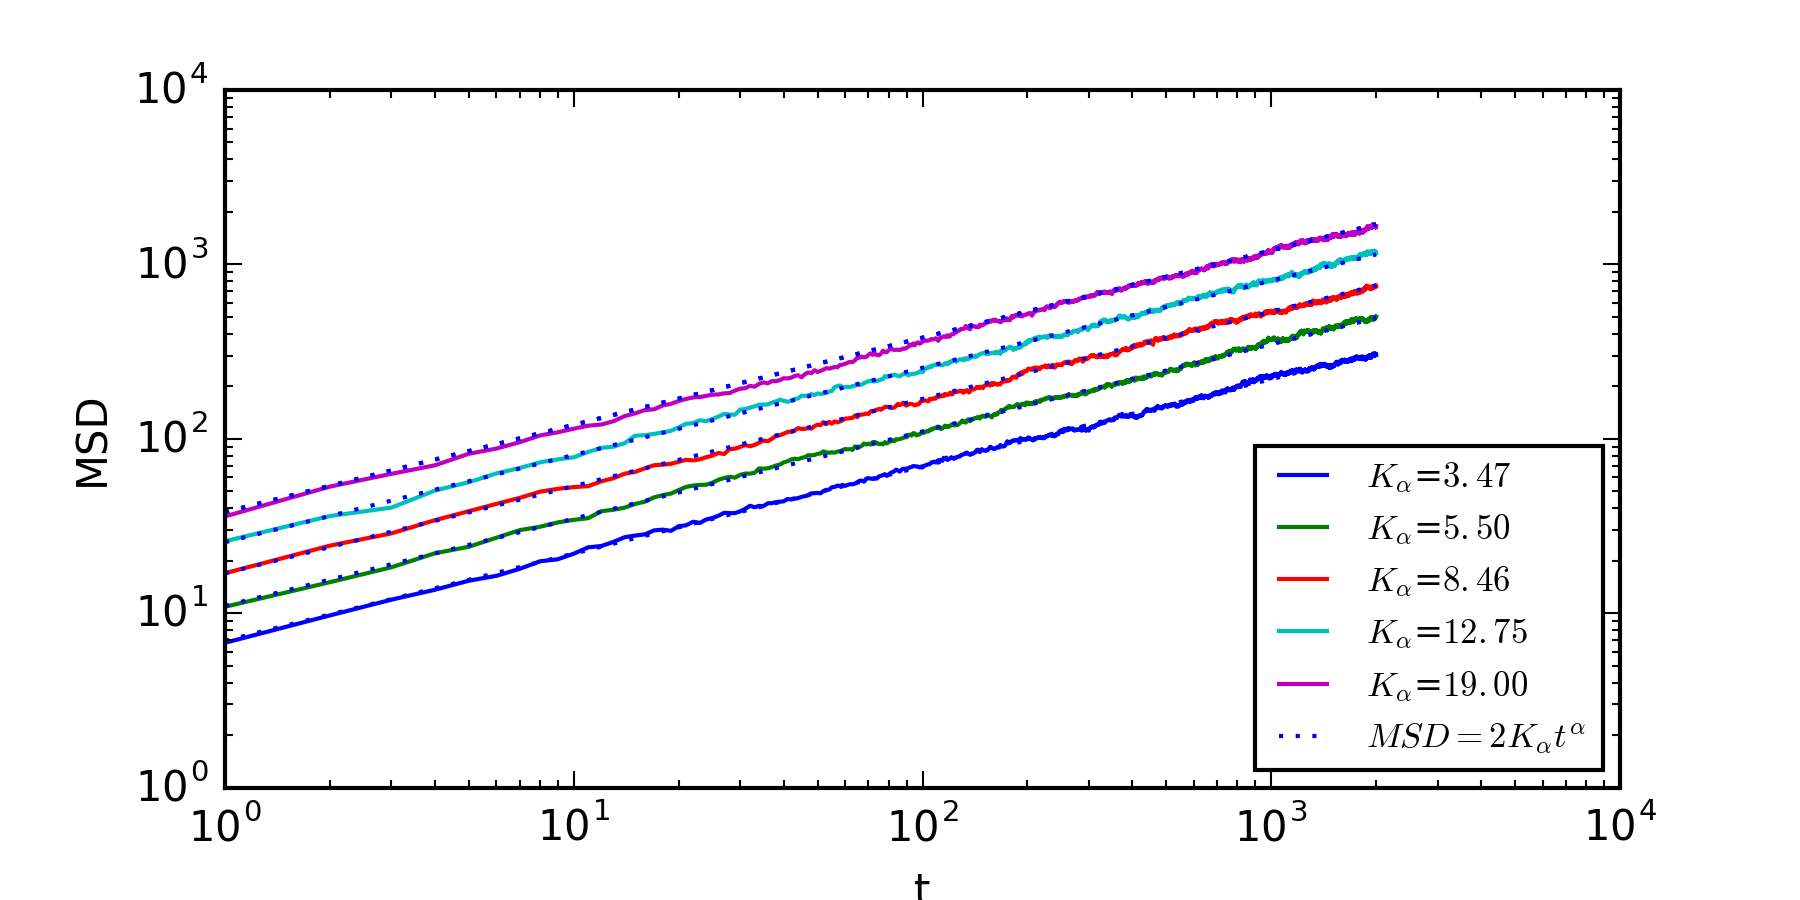
\includegraphics[width=\textwidth]{./data/K_alpha_change.png}
\caption{Ensemble averaged MSD for different $K_\alpha$. with $\alpha=0.5$ , $N=2000$, $n=2000$ , $\Delta t = 1$, $M=2n$.}
\label{kalphachange}
\end{figure}
\noindent The generalized diffusion coefficient has also bin varied. The influence on the MSD can be seen in \cref{kalphachange} . The change of $K_{alpha}$ is not influencing the quality of the simulation.
\begin{figure}[h!]
\begin{minipage}{\textwidth}
\centering
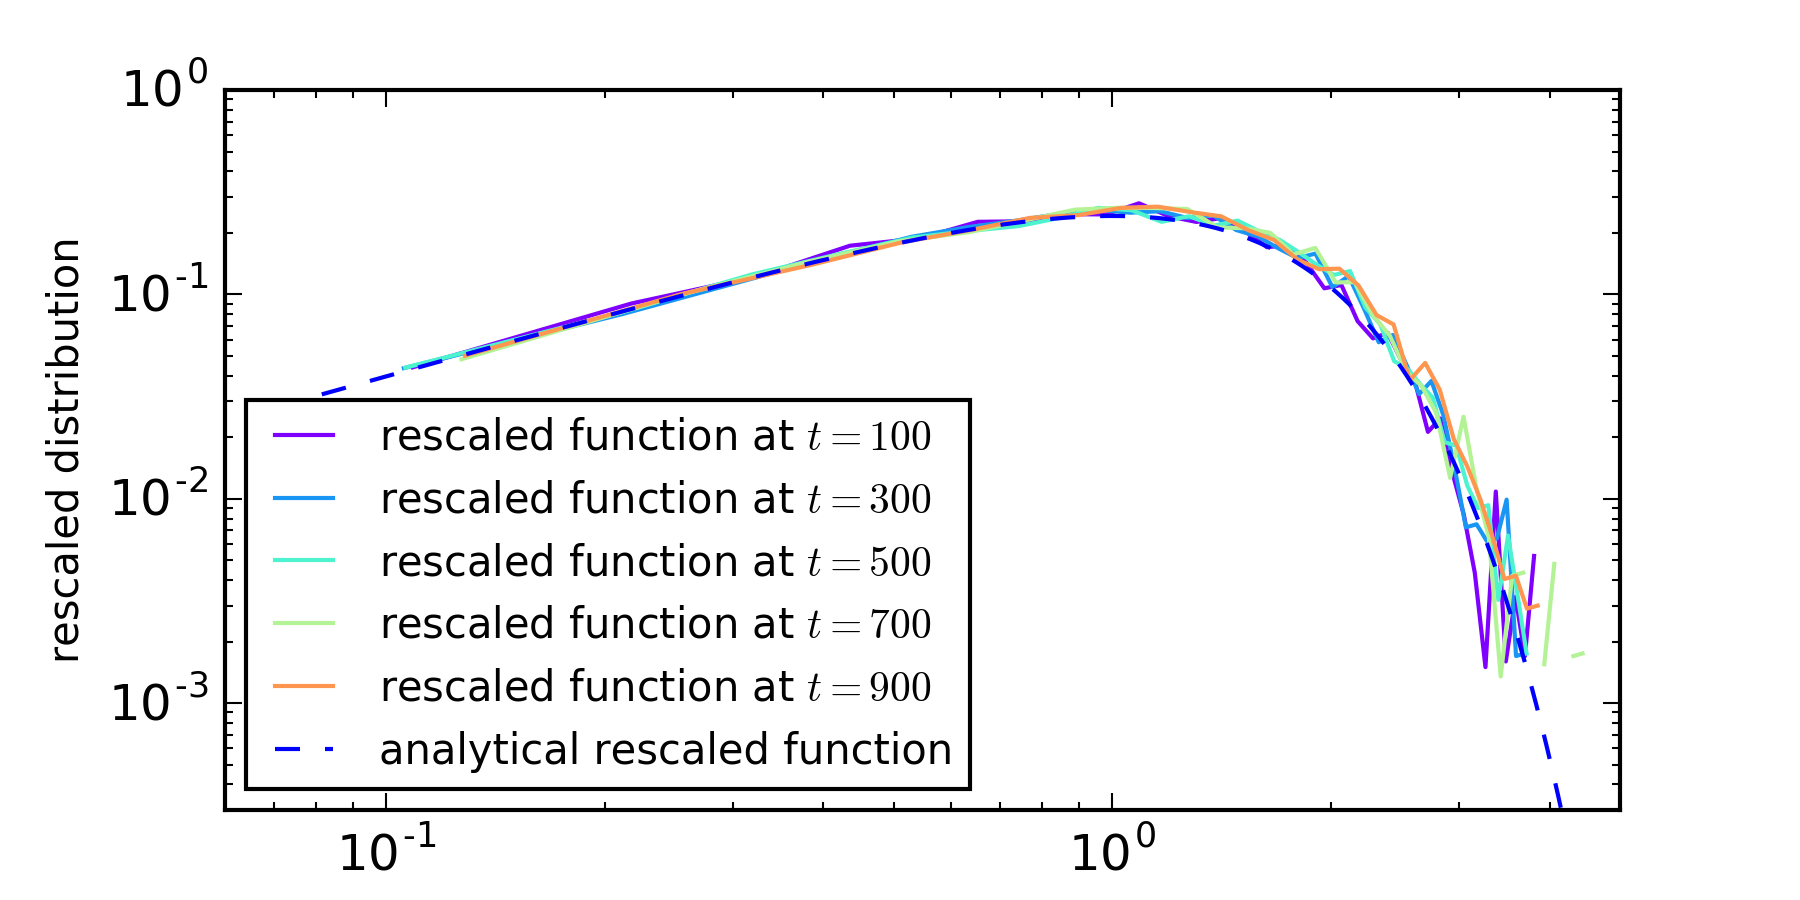
\includegraphics[width=\textwidth]{./data/rescaled.png}
\caption{The scale free form of the Propagator at different times as introduced in \cref{scalefreeformfrac}. With $K_{\alpha}=2$, $\alpha=0.5 $, $N=10000$ , $\Delta t = 1$, $M=2n$.  }
\label{rescaledfigure}
\end{minipage}
\begin{minipage}{\textwidth}
\centering
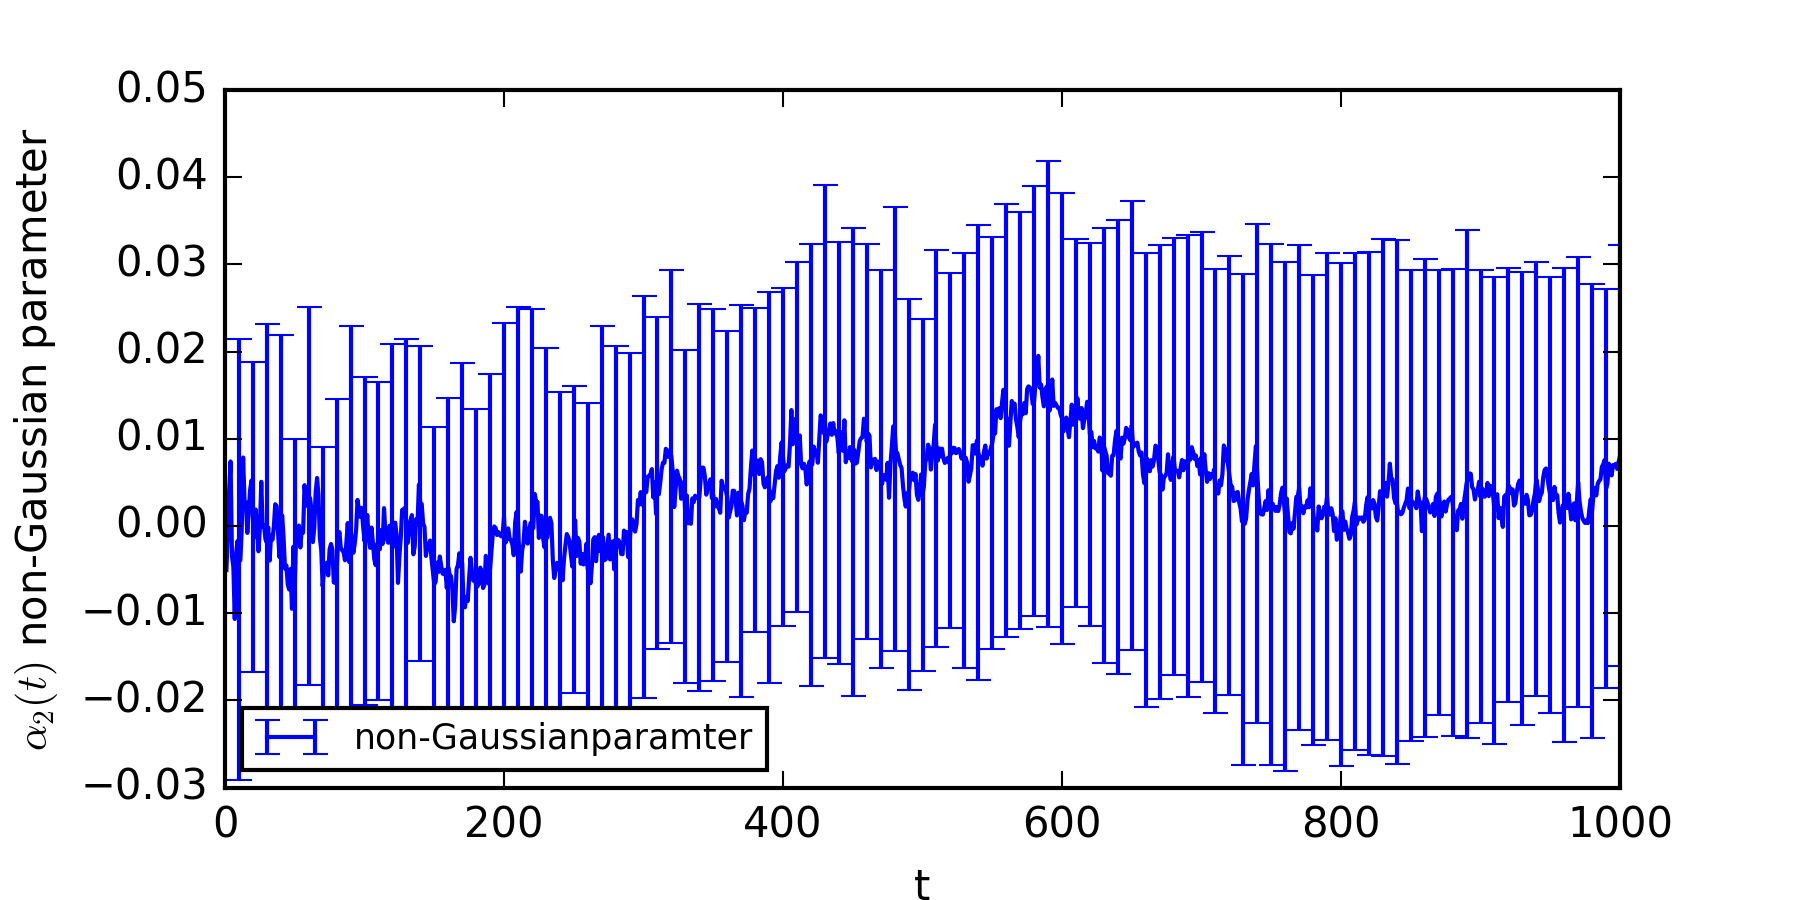
\includegraphics[width=\textwidth]{./data/nongaussian.png}
\caption{Non-Gaussian-Parameter (as introduced in \cref{nongaussian2}) With $K_{\alpha}=2$ , $N=5000$, $n=1001$ , $\Delta t = 1$, $M=2n$ averaged over $30$ non-Gaussian-Parameter with its variance displayed as an error bar.}
 \centering
\end{minipage}
\end{figure}

\begin{figure}[h!]
\centering
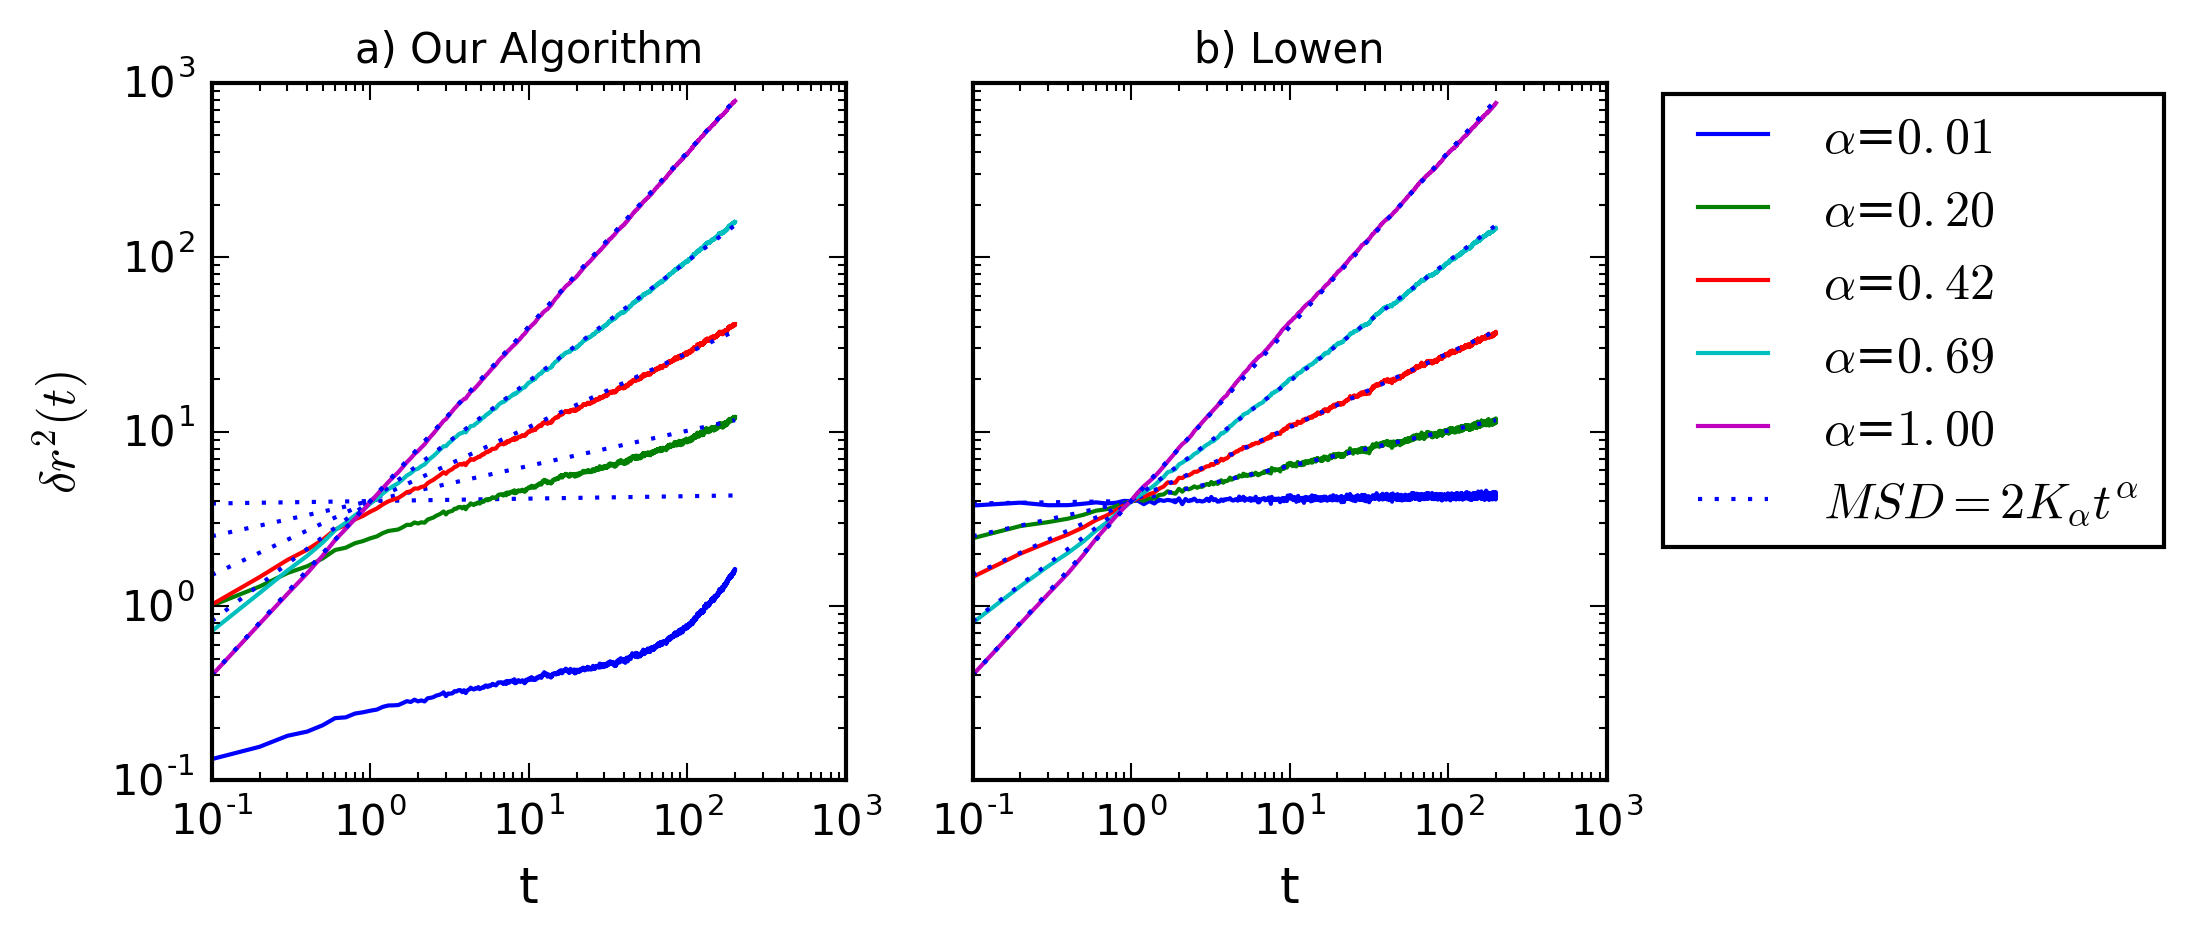
\includegraphics[width=\textwidth]{./data/alpha_changeboth.png}
\caption{Both Plots show an ensemble average MSD over $N=2000$ trajectories for $0.1<\alpha<1.0$  with $K_{\alpha}=2$ , $M=2000$ , $\Delta t = 0.1$, with a) Our algorithm and b) Lowen algorithm.}
\label{alphachange}
\end{figure}
\noindent As a property of self similarity a scale free version of the density distribution can be calculated \cref{sectionfrac} \cref{scalefreeformfrac}. The scale free density distribution is not depended on time but overlaps for all times. The algorithm is performing as predicted and computing a self-similar process. The scale free distribution is extracted from the simulation for different times and compared to the analytical result. The graph can be seen in \cref{rescaledfigure}.  

 
\end{comment}


\begin{figure}[h!]
\centering
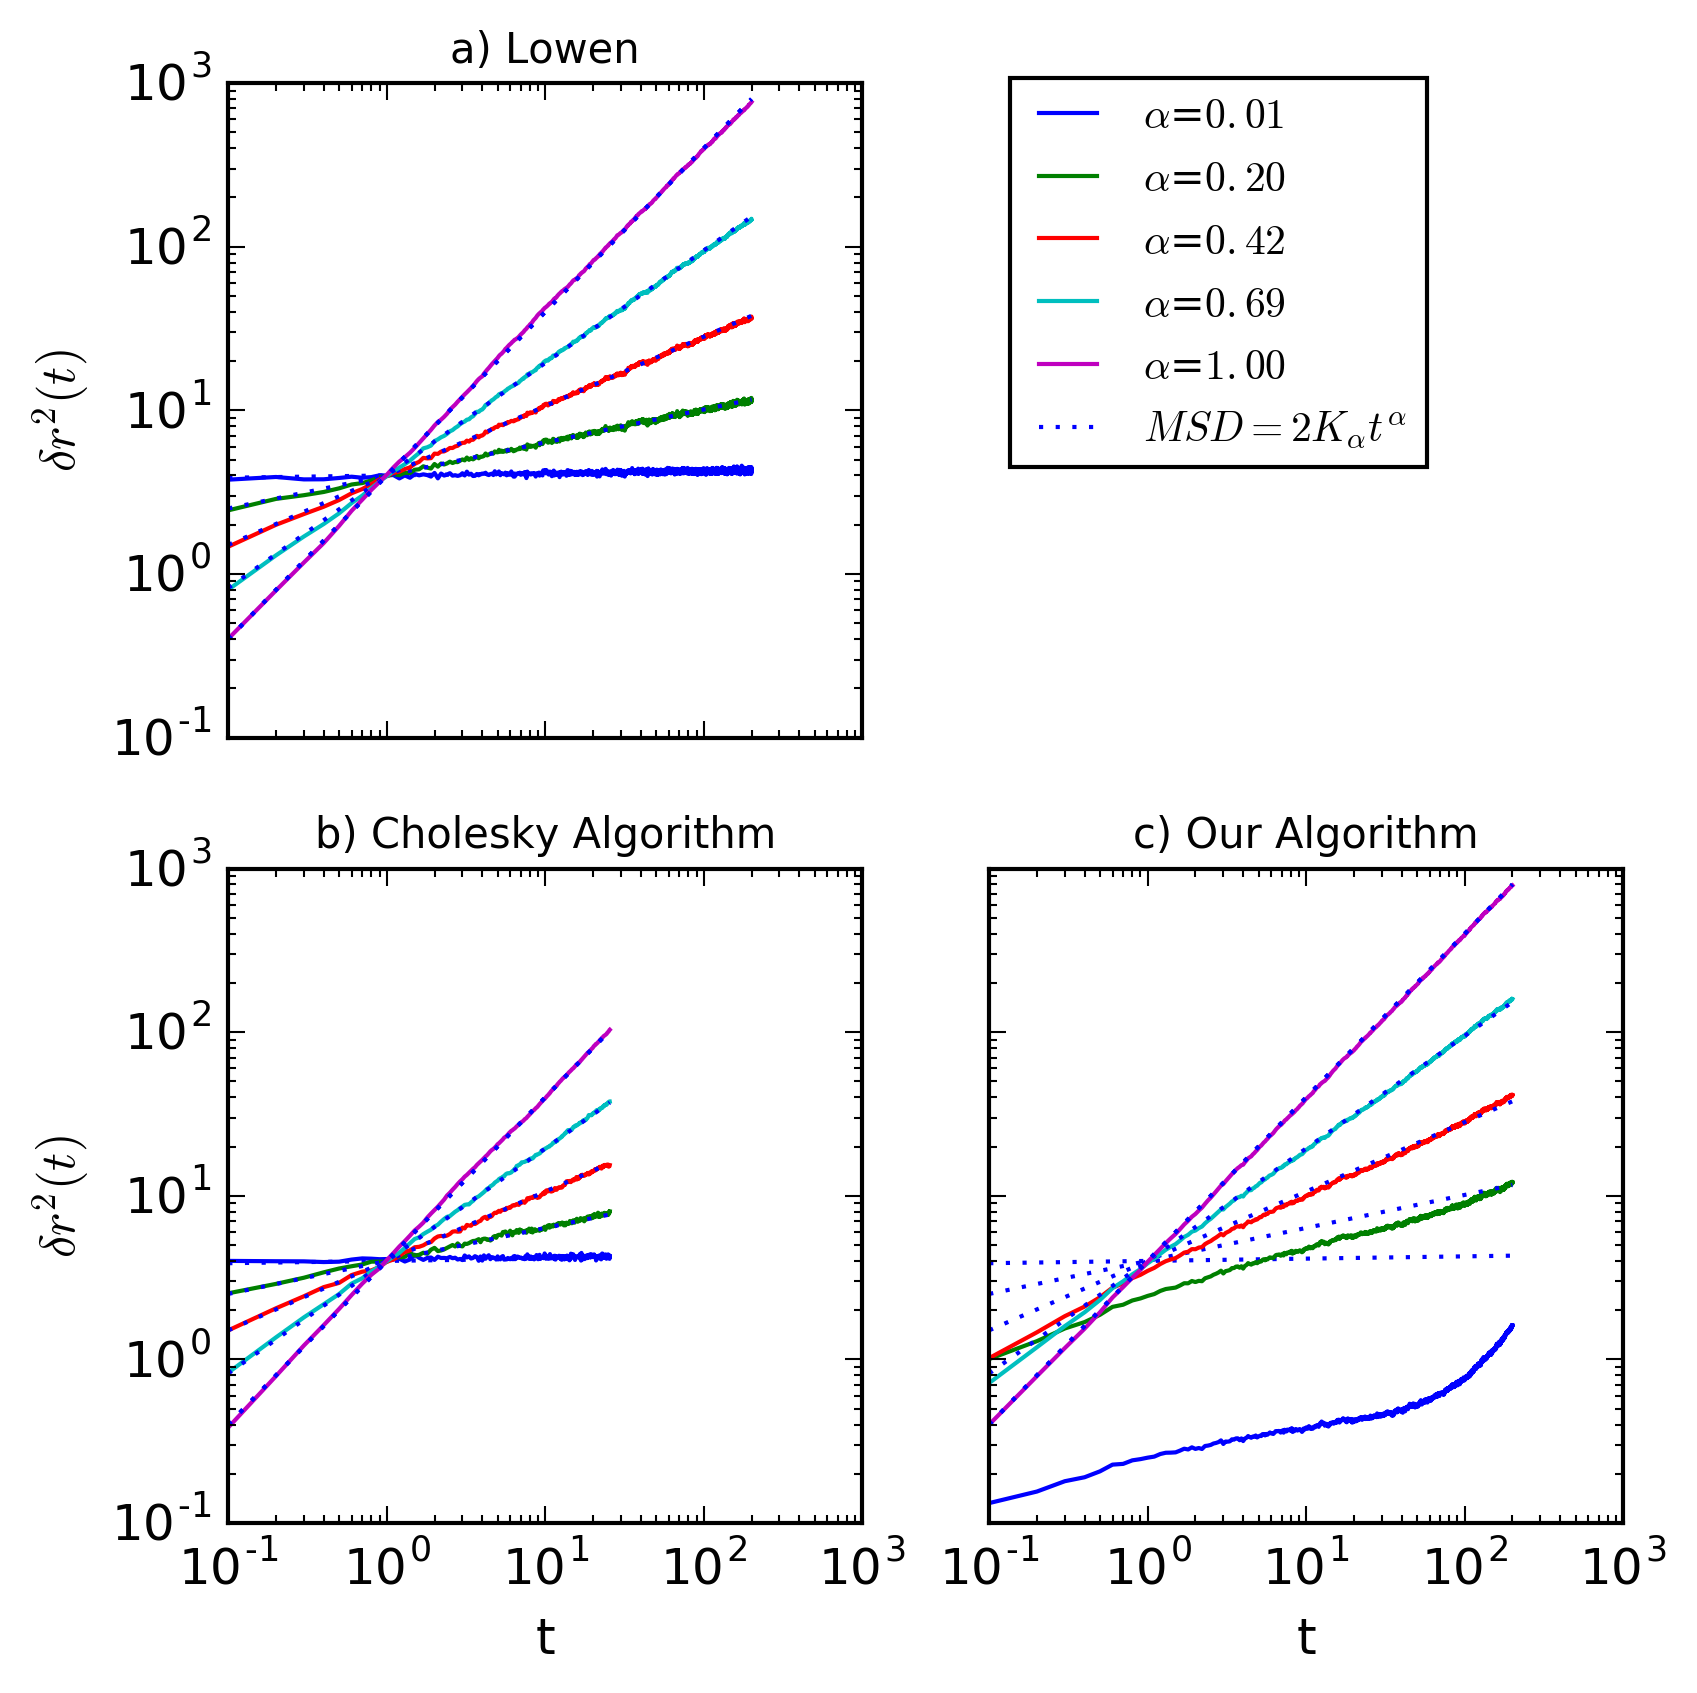
\includegraphics[width=\textwidth]{./data/alpha_changethree.png}
\caption{All three plots show an ensemble averaged MSD over $N=2000$ trajectories for $0.1<\alpha<1.0$  with $K_{\alpha}=2$ ,$\Delta t = 0.1$ and trajectory length $M=2000$  for Our and Lowen algorithm, $M=256$ for Cholesky algorithm. a) Our algorithm and b) Lowen algorithm c) Cholesky algorithm.}
\label{alphachange}
\end{figure}

FBms property of self similarity can be used to plot a scale free version of the density distribution. The scale free version was introduced in \cref{scalefreeformfrac}. The scaled density distribution is not depended on time but overlaps for all times. In \cref{rescaledfunction}  histograms over $N=10000$ single trajectories at various times ($100\leq t \leq 1000$) were calculated and rescaled according to \cref{scalefreeformfrac}. The dashed line show the expected distribution. For Cholesky and our algorithm no deviations from the analytical line is obvious. For Lowens algorithm systematically small changes to the analytical value can be observed. However, the distribution of fBm should stay a Gaussian for all times.  As introduced in \cref{nongaussian2} the non-Gaussian parameter should be zero. The Non-Gaussian parameter has been plotted for $0 \leq t \leq 1000 (\leq 356 \text{ for Cholesky})$  $\alpha=0.5$  in \cref{nongaussianlowen} a). Our and Cholesky algorithm perform as expected. Lowen however show deviation from a Gaussian distribution increasingly towards the end of the trajectory. In  \cref{nongaussianlowen} b) the influence of $\alpha$ on the non-Gaussian parameter for the Lowen algorithm was tested. For small $\alpha$ the distribution is closer to a Gaussian. In our implementation Lowens algorithm is not exact as claimed in \cite{Lowen1999}.

\begin{figure}[h!]
\centering
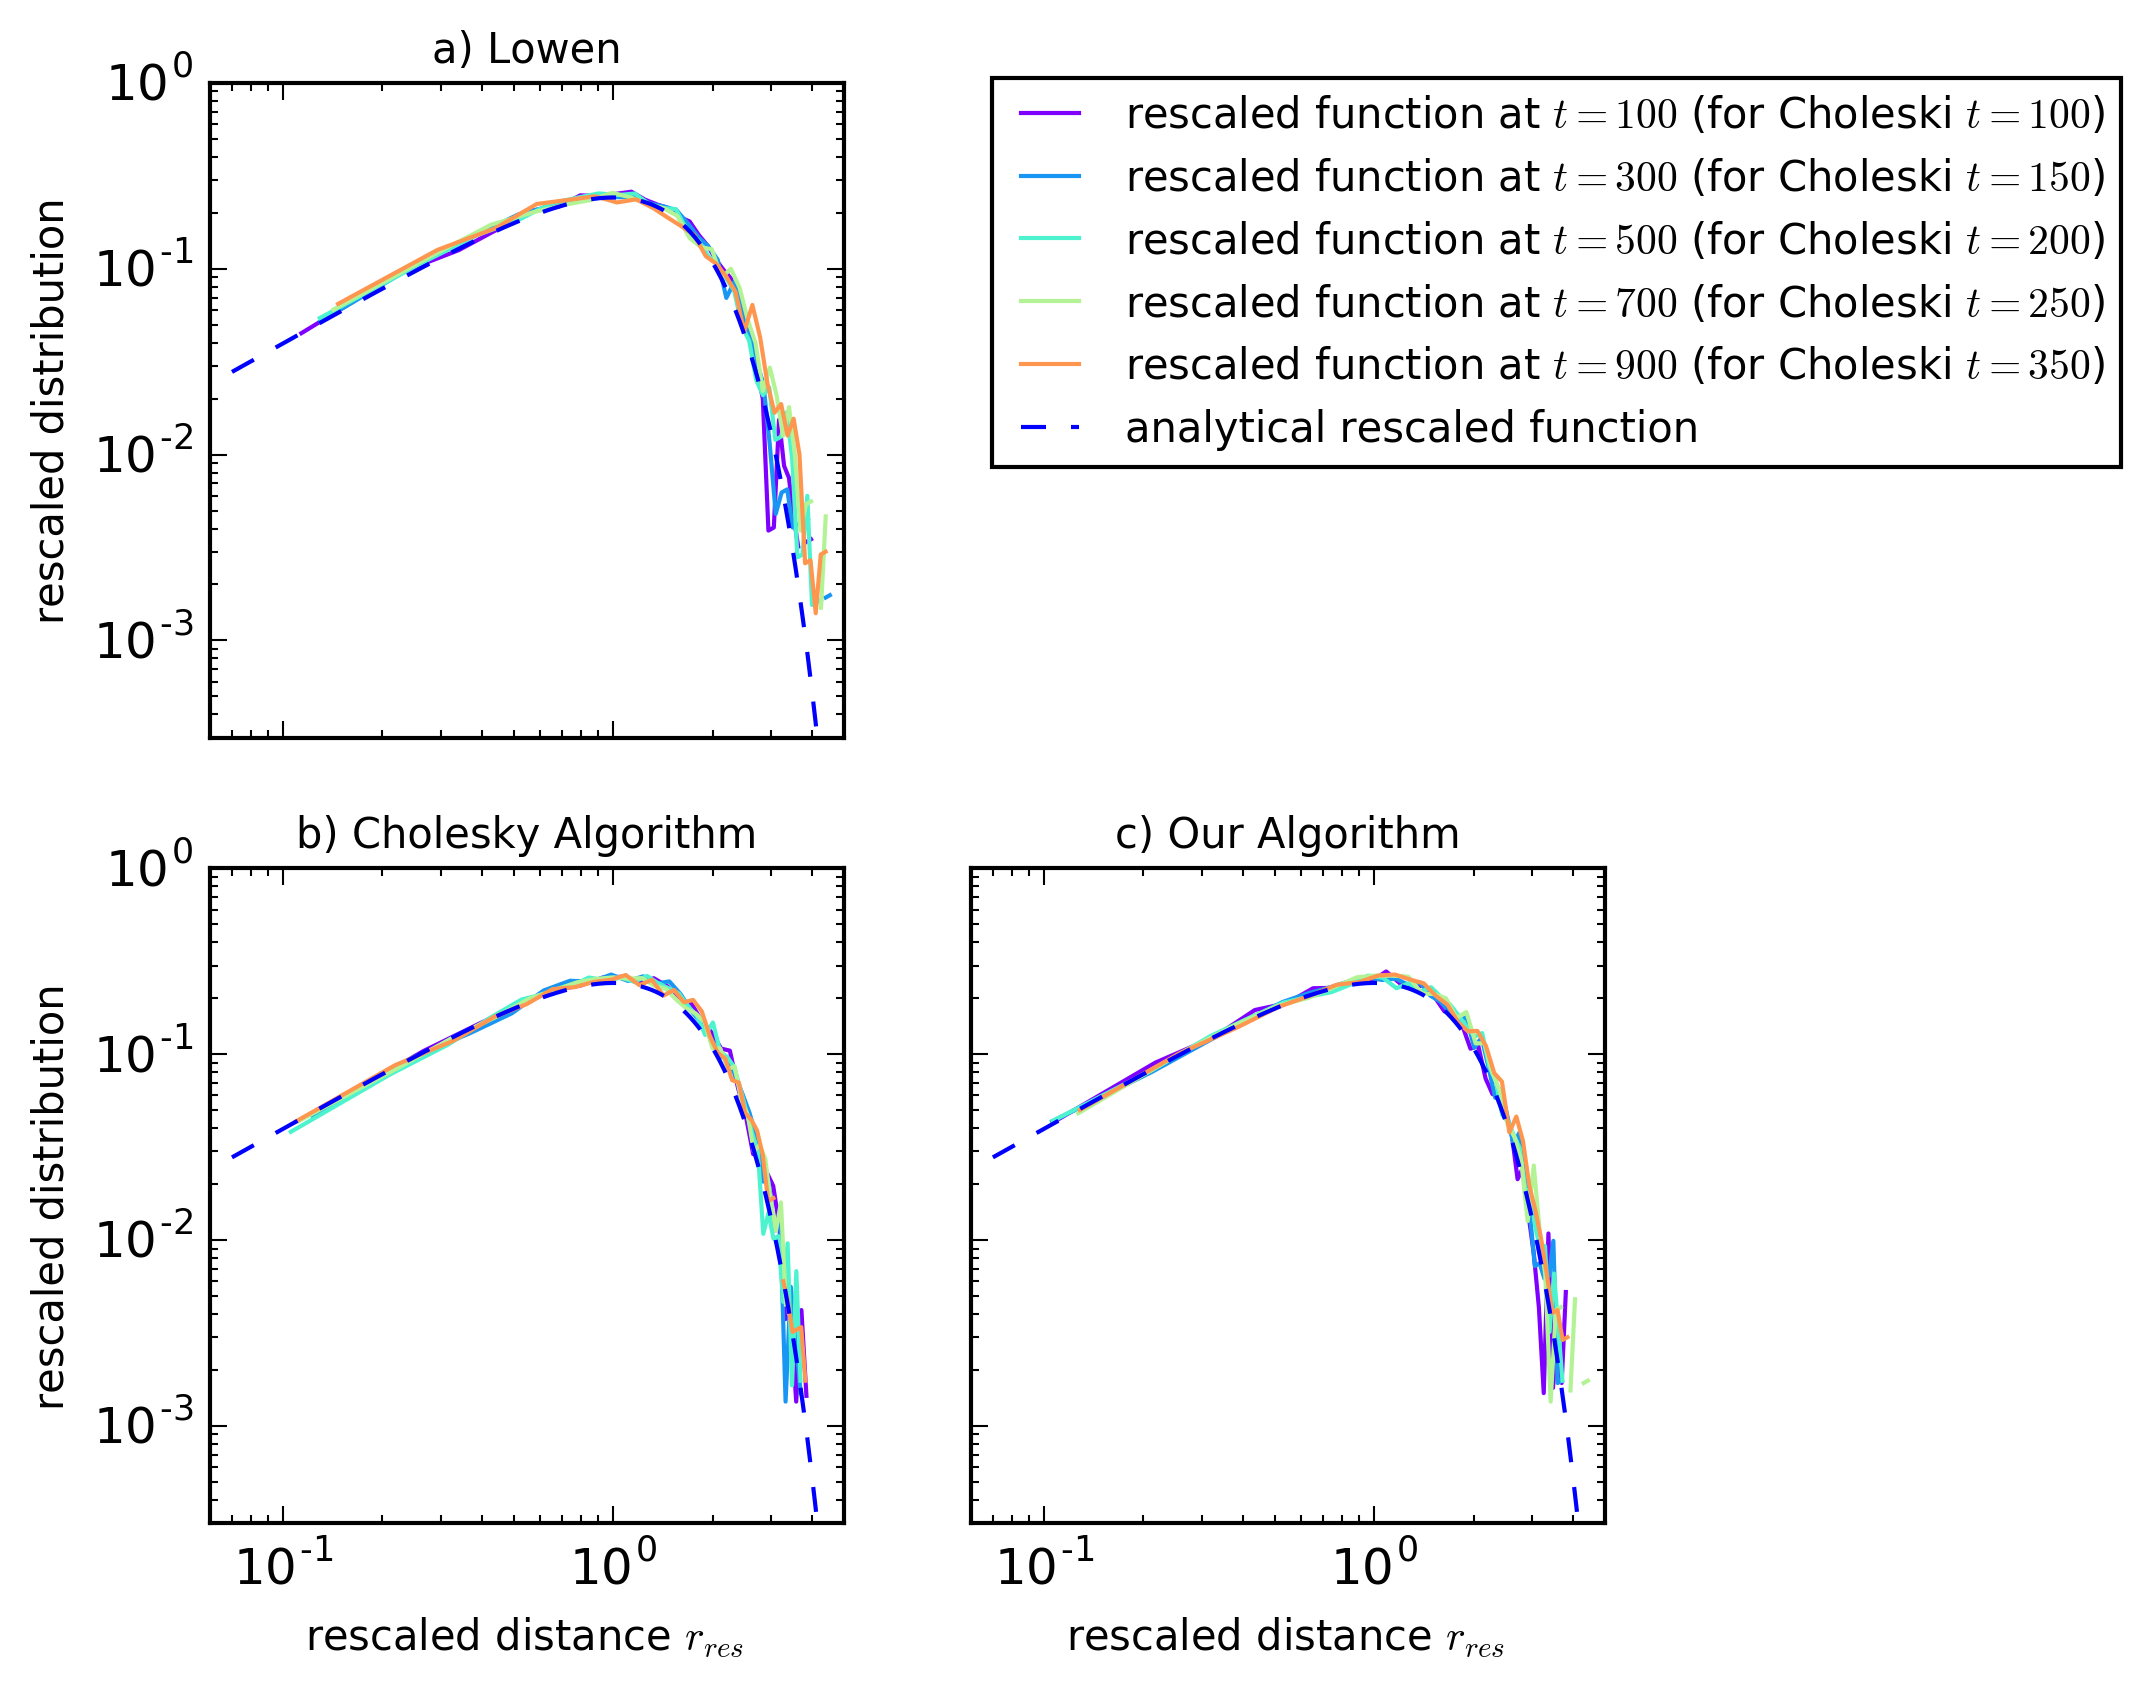
\includegraphics[width=\textwidth]{./data/scaledfunctionneu.png}
\caption{All three plots show the scale free form of the propagator at different times as introduced in \cref{scalefreeformfrac} as an histogram over $N=10000$ trajectories for $\alpha=0.5$  with $K_{\alpha}=2$ ,$\Delta t = 0.1$ for all three algorithm, at different times $100<t<900$}
\label{rescaledfunction}
\end{figure}

 
\begin{comment}
 

\begin{figure}[h!]
\centering
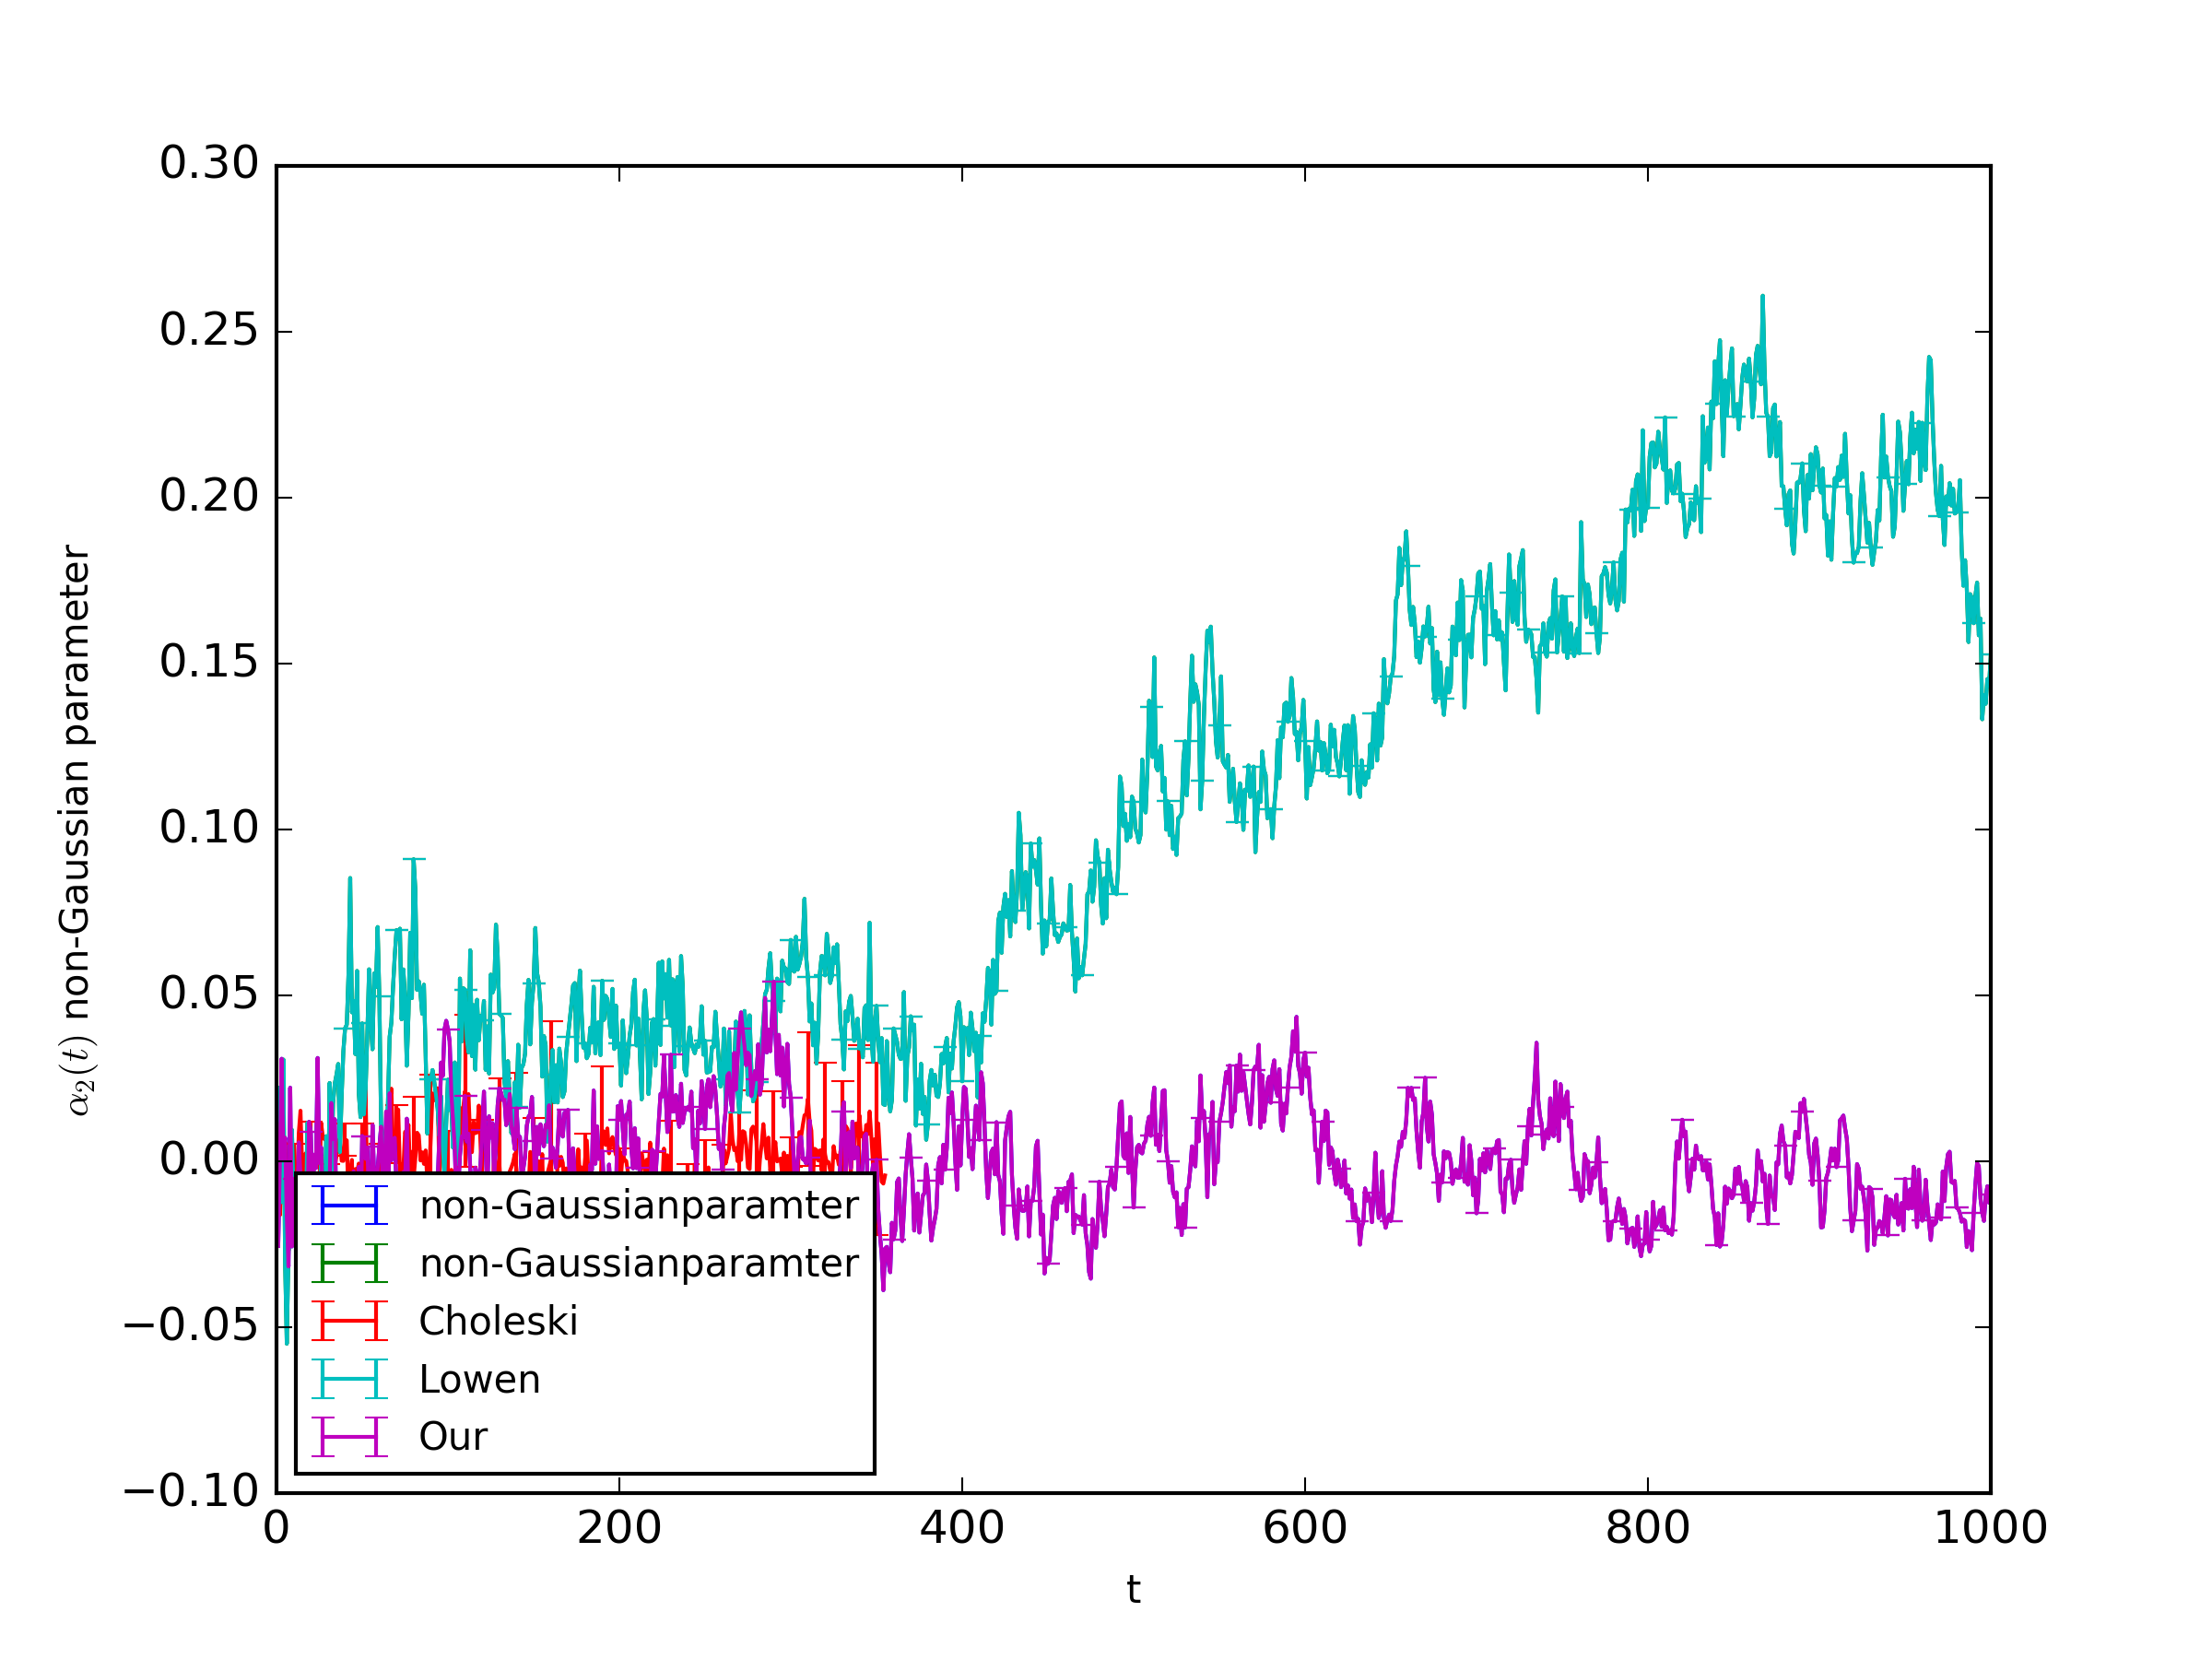
\includegraphics[width=\textwidth]{./data/nongaussianneu.png}
\caption{a) Non-Gaussian-Parameter as introduced in \cref{nongaussian2} for all three algorithms with $K_{\alpha}=2$ , $N=5000$,$\alpha=0.5$ (Lowen and Our $M=1001$; Choleski $M=356$), $\Delta t = 1$  averaged over $50$ non-Gaussian-Parameter with its variance displayed as an error bar.}
\label{nongaussian}
\end{figure}
\end{comment}

\begin{figure}[h!]
\centering
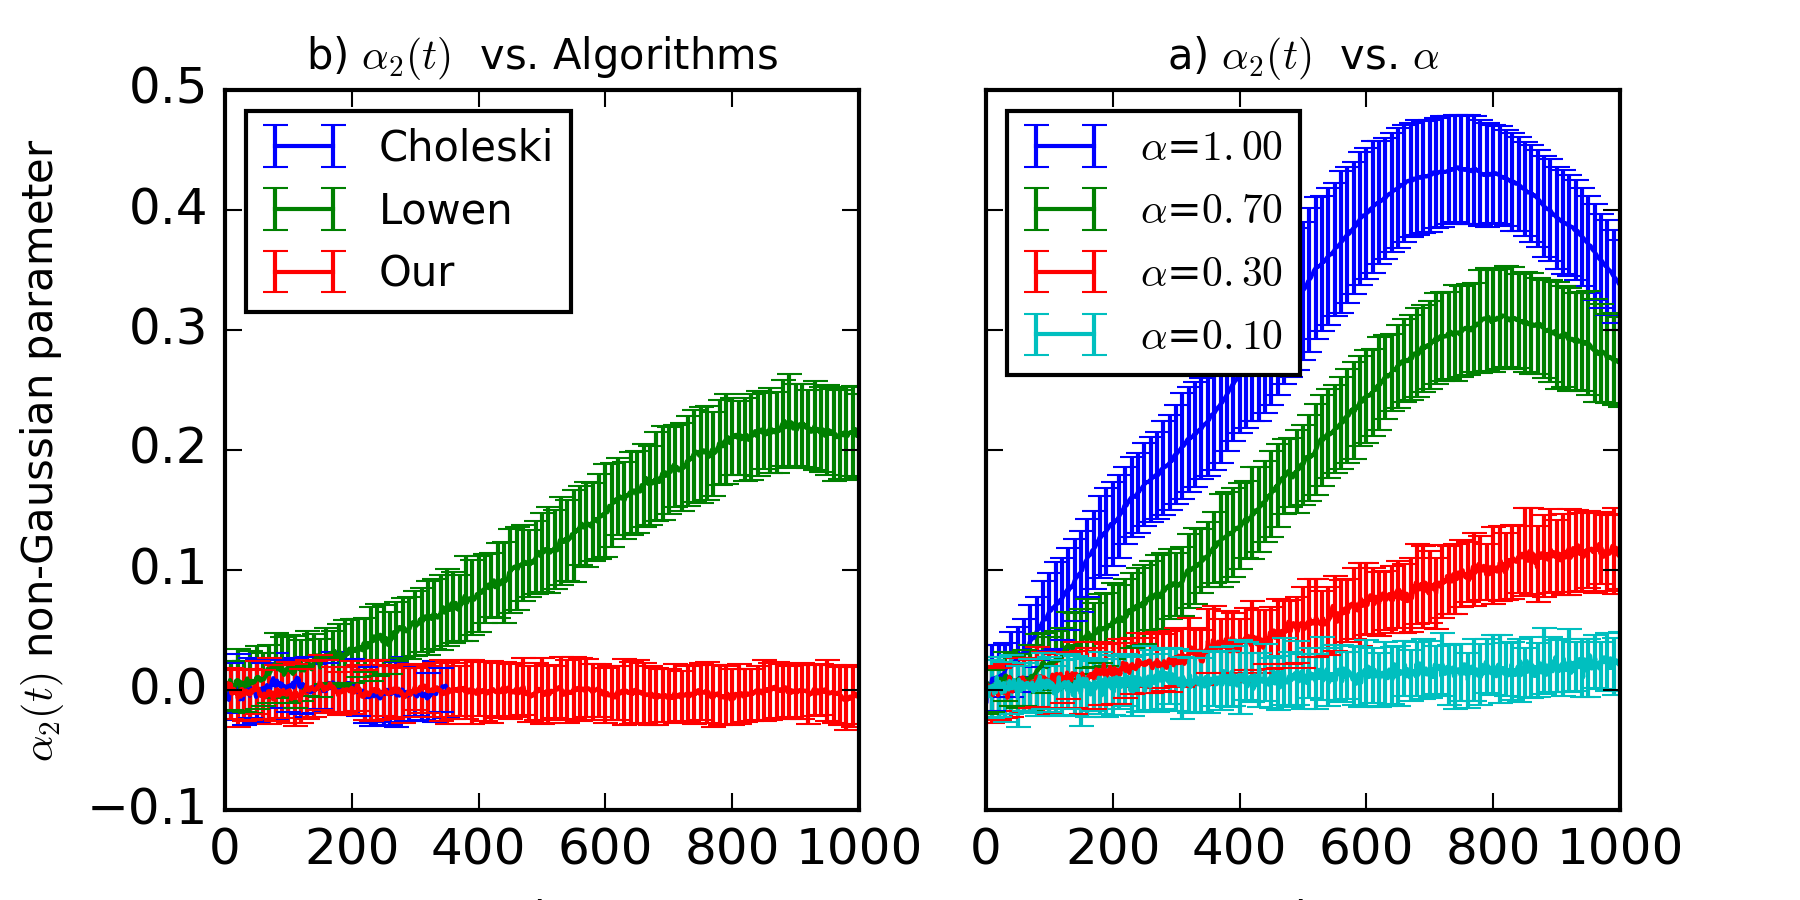
\includegraphics[width=\textwidth]{./data/nongaussianlowenalpha.png}
\caption{a) Non-Gaussian-Parameter as introduced in \cref{nongaussian2} for all three algorithms with $K_{\alpha}=2$ , $N=5000$,$\alpha=0.5$ (Lowen and Our $M=1001$; Cholesky $M=356$), $\Delta t = 1$  averaged over $50$ non-Gaussian-Parameter with its variance displayed as an error bar.\newline
b) Non-Gaussian-Parameter for Lowen algorithms with $K_{\alpha}=2$ , $N=5000$, $M=1001$, $\Delta t = 1$ and for various $0.1\leq\alpha\leq1.0$  averaged over $50$ non-Gaussian-Parameter with its variance displayed as an error bar.}
\label{nongaussianlowen}
\end{figure}

\begin{comment}

\begin{figure}[h]
  \centering
  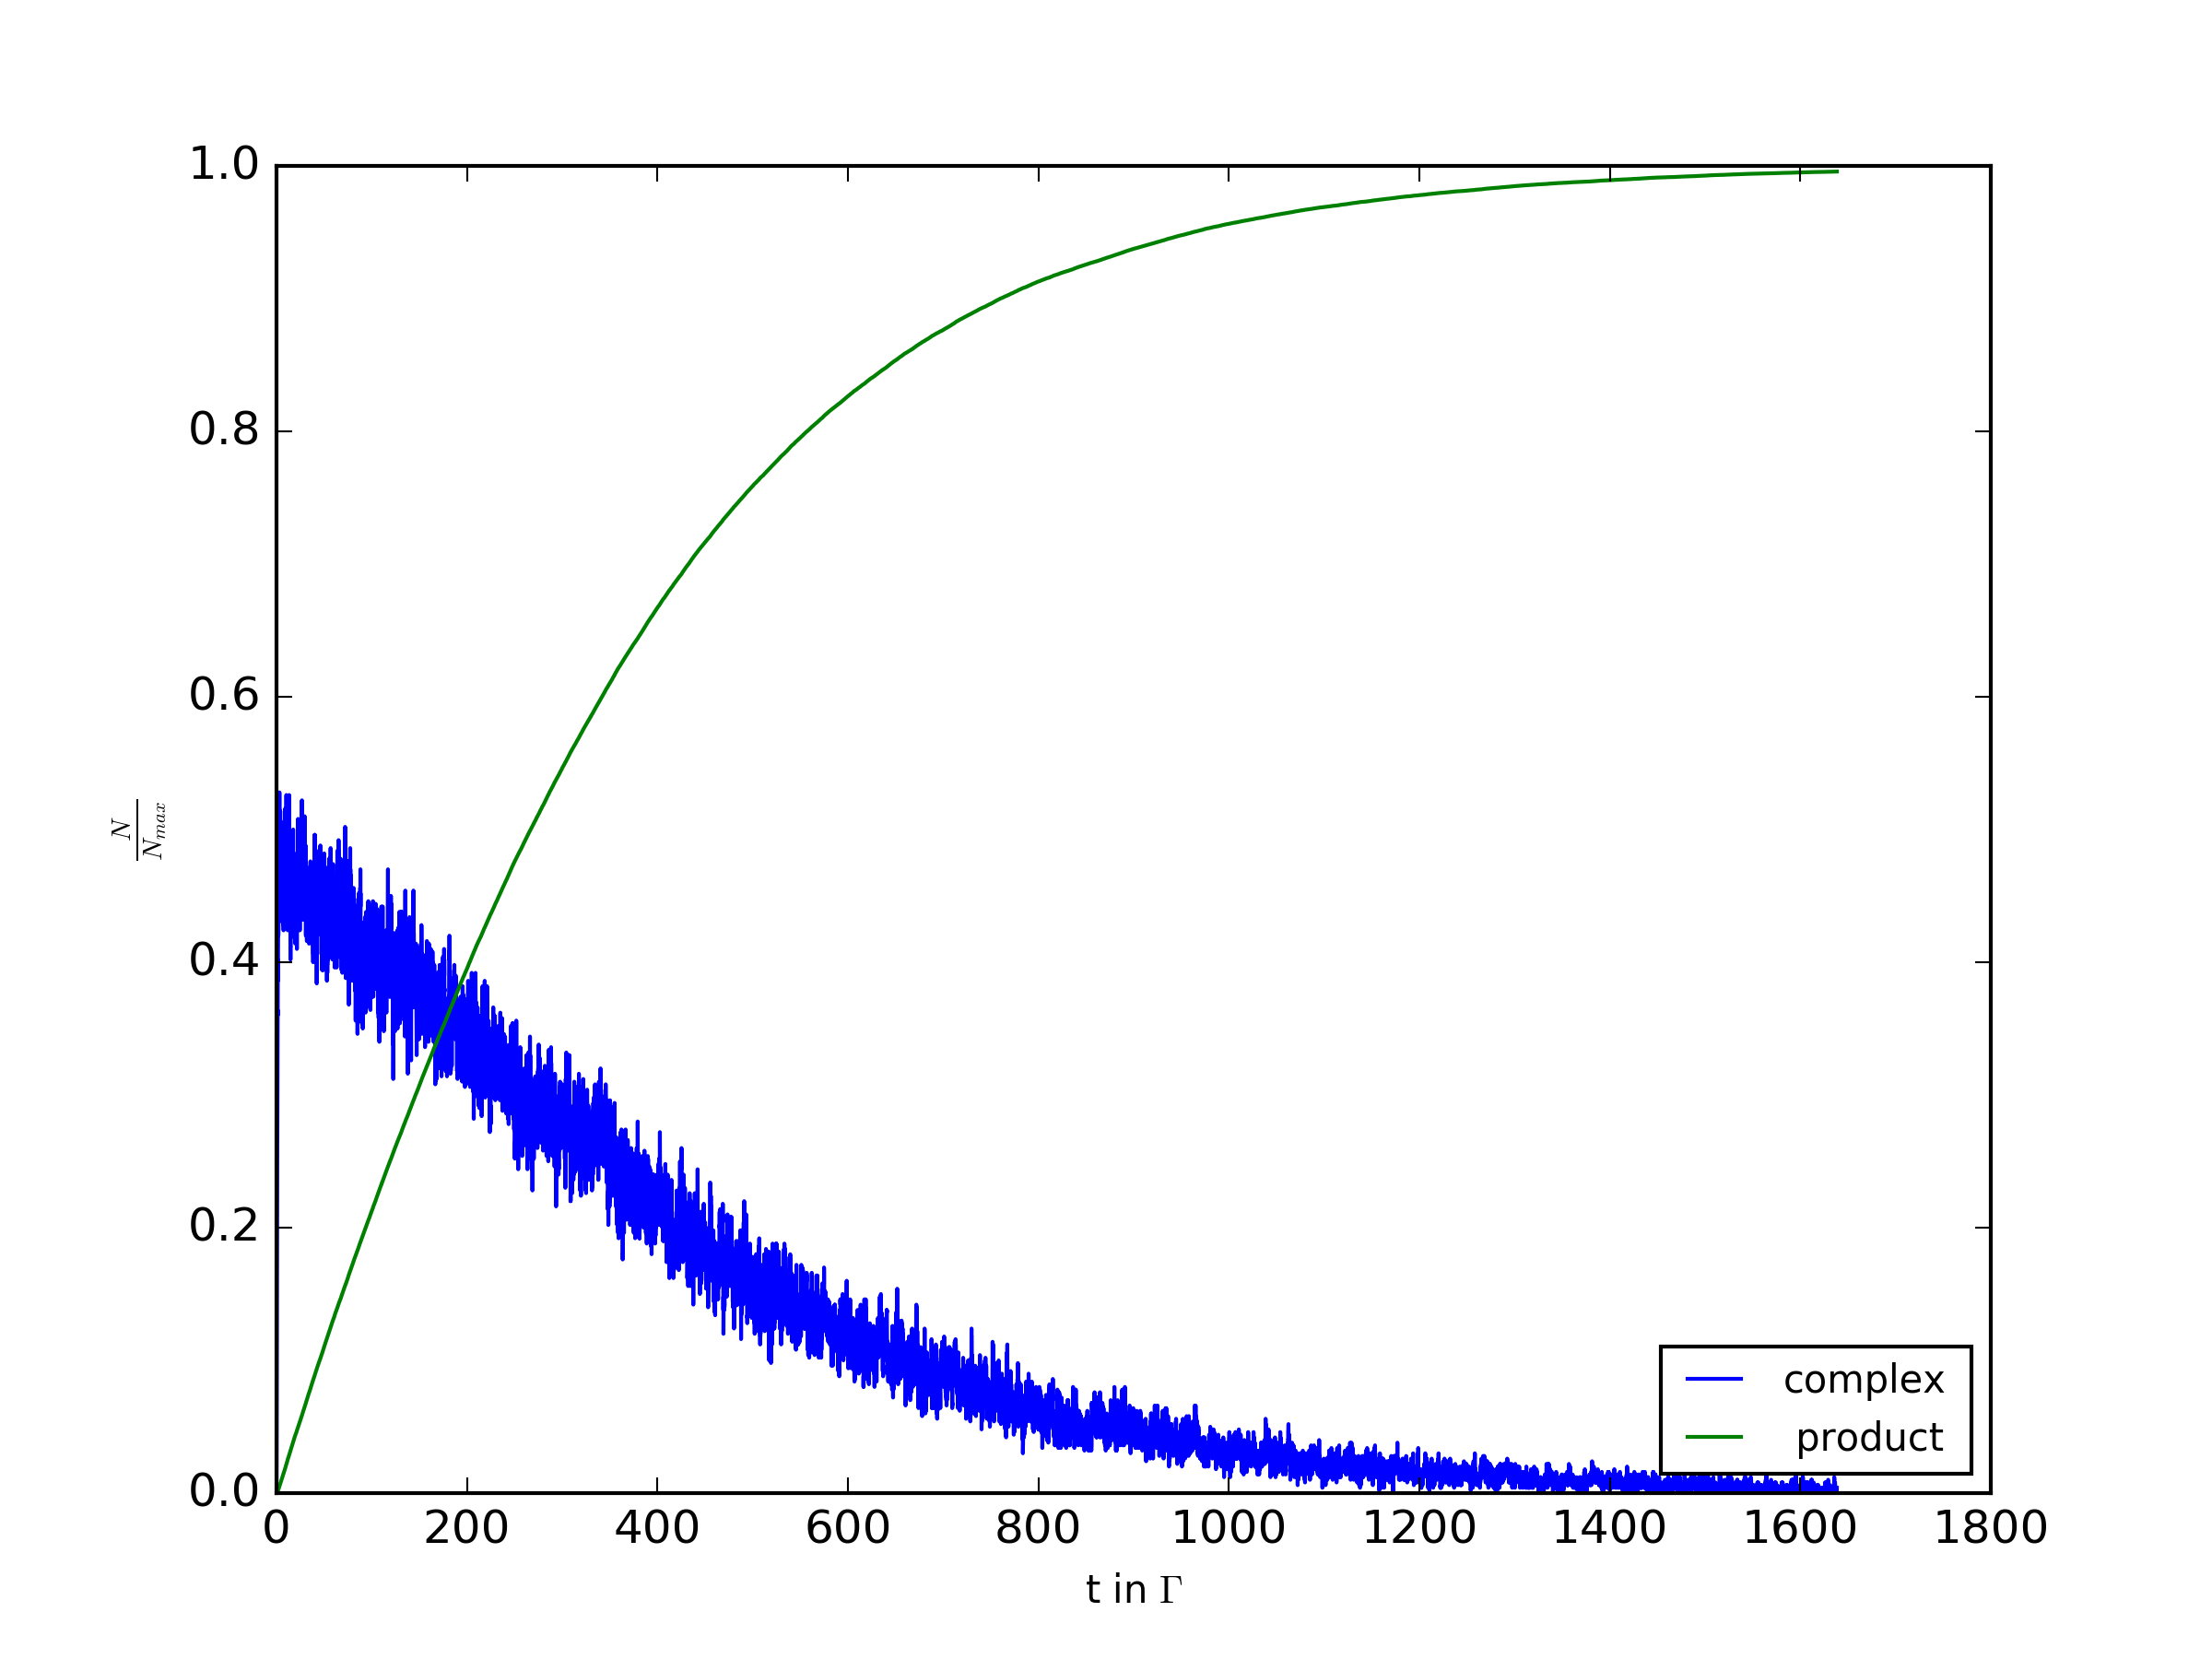
\includegraphics[width=\linewidth]{./data/profiling_length.png}
  \captionsetup{width=0.9\linewidth}
  \captionof{figure}{Scaling behaviour of computational time of both algorithms implemented in c++ and python  in respect to trajectory length $M$,for $N=1$, $t = \mathcal{O}(M log(M))$ }
  \label{fig:1}
\end{figure}
\begin{figure}[h!]
  \centering
  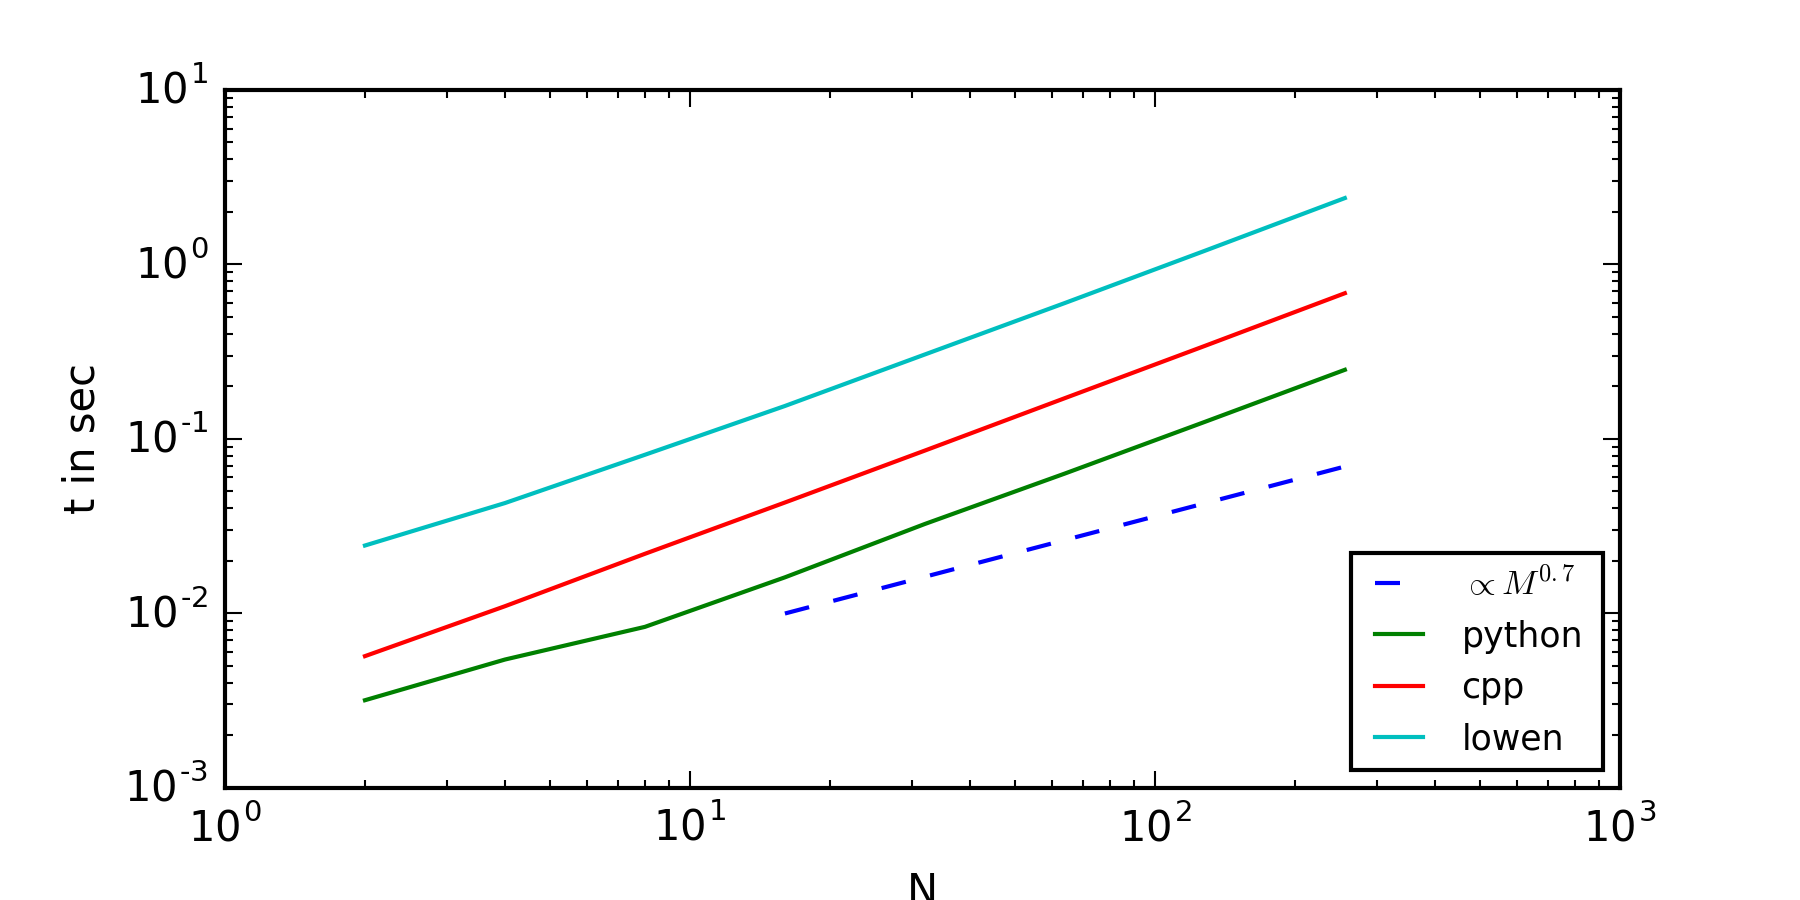
\includegraphics[width=\linewidth]{./data/profiling_particle.png}
  \captionsetup{width=0.9\linewidth}
  \captionof{figure}{Scaling behaviour of computational time of both algorithms implemented in c++ and python  in respect to trajectory number $N$ for $M=1000$ ,$t = \mathcal{O}(N log(N))$}
  \label{fig:2}
\end{figure}
\end{comment}
\newpage
\subsubsection{Performance Analysis}
The performance in respected to sample size (trajectory length) and number of samples (amount of trajectories) was analyzed in \cref{fig:200} b) . Thereby the most promising, in terms of exactness, Cholesky algorithm scales in respect to the trajectory length $M$ with $\mathcal{O}(M^3)$. Our application of the integrator desire long trajectories. It is not reasonable to use such a slow algorithm. Even if every next trajectory with the same $\alpha$ and length is of  $\mathcal{O}(M^2)$ \cite{Dieker2004}. In \cref{fig:200} a) one can see Cholesky to scale slow with the amount of trajectories $N$. Although one should keep in mind that the trajectory length had to be chosen $M=128$ compared to $M=1000$ as for Our and Lowens algorithm to get comparably small values. Lowens and Our algorithm perform both $\mathcal{O}(M log(M))$ in respect to the trajectory length as a result of the FFT and $\mathcal{O}(N)$ in respect to the amount of trajectories.
\begin{figure}[h!]
  \centering
  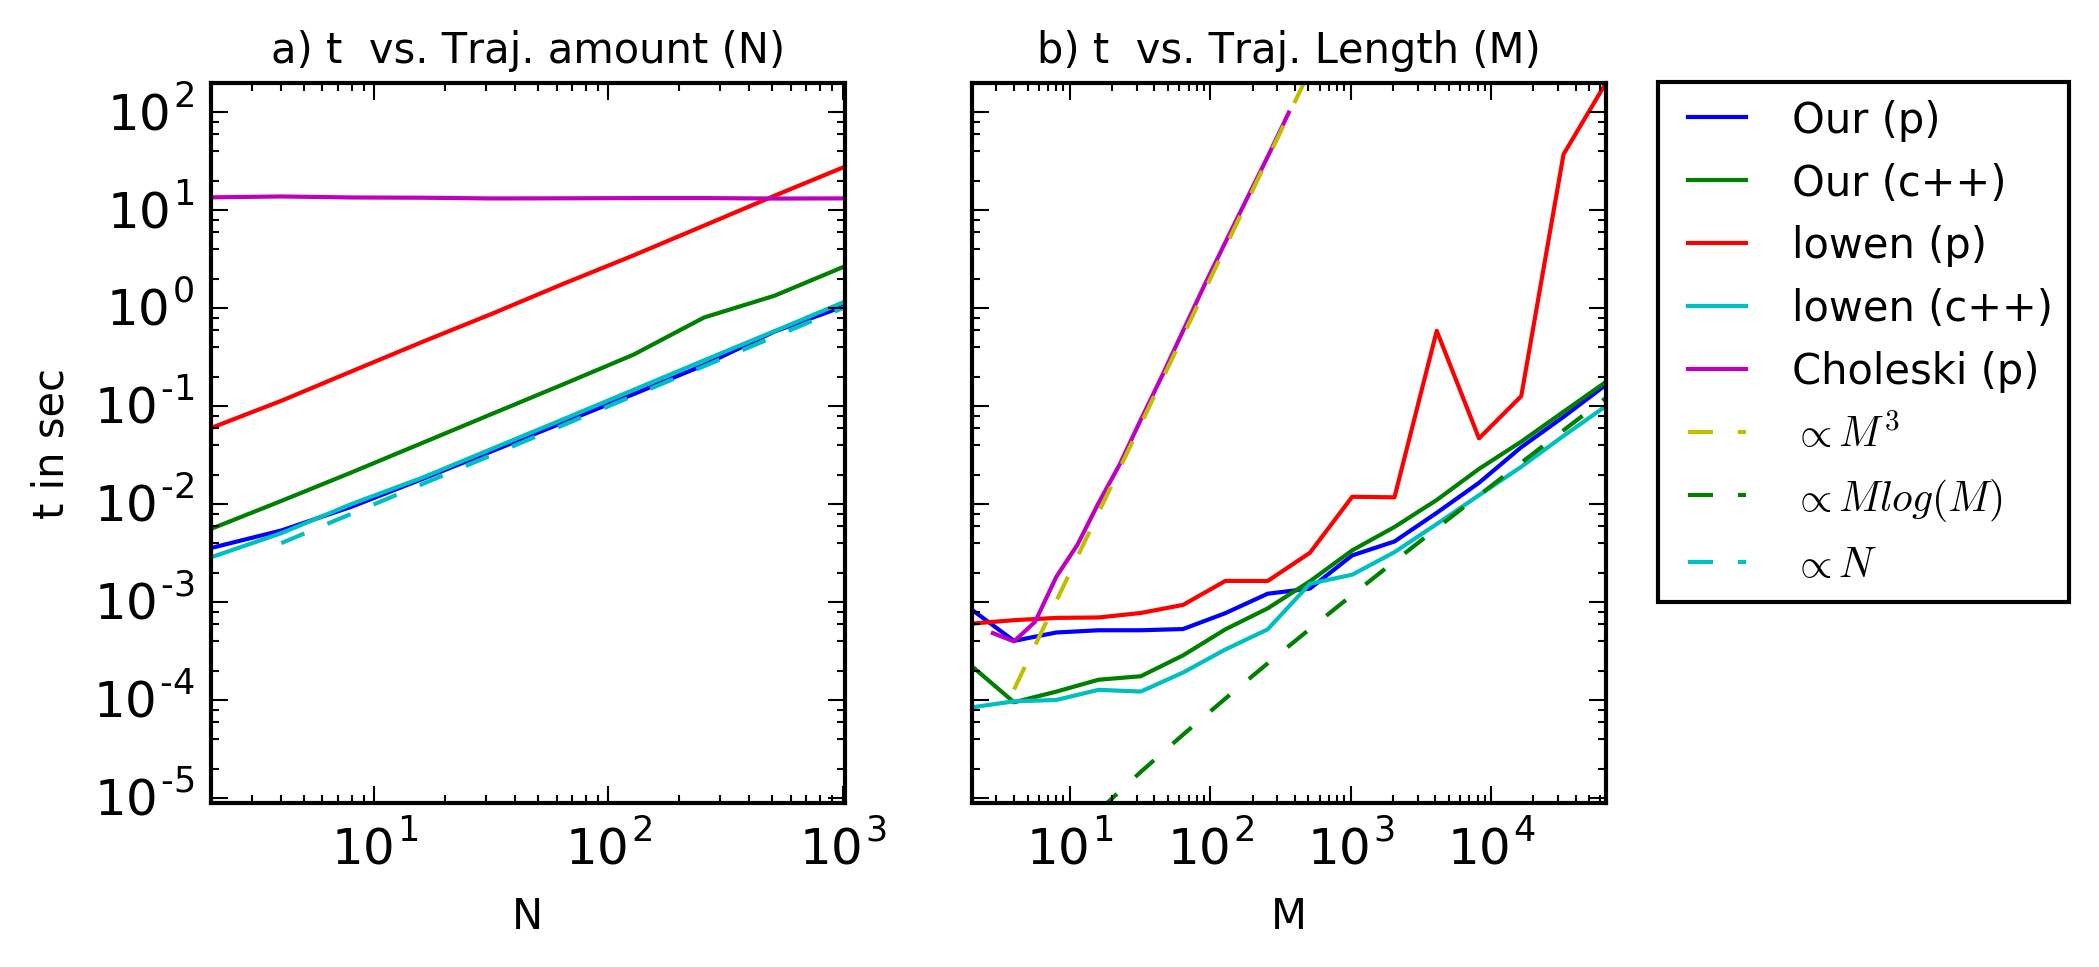
\includegraphics[width=\linewidth]{./data/profilingneu1.png}
  \captionsetup{width=0.9\linewidth}
  \captionof{figure}{a) Algorithmic scaling of computational time in respect to the amount of trajectories $N$ for trajectory length $M=1000$ , ($D=2$, $\alpha=0.5$, $\Delta t=1$) of Lowen and our own algorithm. Both implemented in  c++ and python (p). The Cholesky algorithm was implemented in python with $M=128$.\newline
  b) Algorithmic scaling of computational time in respect to the trajectory length $M$ for a single trajectory $N=1$ , ($D=2$, $\alpha=0.5$, $\Delta t=1$). Lowen and our own algorithms are implemented in c++ and python (p). Cholesky is only implemented in python (p).}
  \label{fig:200}
\end{figure}

\chapter{Particle Based Reaction Diffusion }
Chemical reactions are ubiquitous in nature. They describe transformations of one or several chemical substances. Transformations of chemical substances are described by formation and breaking of chemical bonds. Physically correct theses bonds should be described quantum mechanically. Quantum mechanics is not needed for a description at cellular scales. Not to mention that for such large systems these calculation cannot be performed. Hence, coarse grained models for reactions at cellular scale were developed. But reactions in a broader sense can also be a transformations of one state to another one (e.g. protein changing its conformation). Biochemical reaction give rise to the complexity of life and are of key importance for processes in living cells. Enzymatic reactions as an example are involved in storage and release of energy, processes of respiration, vision, muscle contraction, transmission of nerve impulses. Indeed Biochemistry is a whole area of research.\par A  Early pioneer general work on reactions by Guldberg and Waage already in 1864 \cite{Waage1986} resulted in the law of mass action, which states the proportionality of the reaction rate to the product of concentrations for elementary molecular reactions. Thereby spatial resolution is neglected. The system is described in terms of a concentration (well-mixed assumption). The mass action law leads to a deterministic model described by ordinary differential equations (ODEs). Quantities like reaction kinetics and amount of reactants in equilibrium can be obtained. Deterministic models however are not resolving stochastic phenomena. Stochastic models provide a more detailed understanding of the reaction-diffusion processes. Such a description is often necessary for the modelling of biological systems, where small molecular abundances of some chemical species make deterministic models inaccurate or even inapplicable \cite{0704.1908}. Stochastic models based on the mass action law are characterised by the chemical master equation (CME). CME describes the temporal evolution of the probabilities for the system to occupy each different state. The interesting topic of chemical kinetics described by CME will not be part of the elaborations. Nevertheless, for the sake of completeness, it was to be mentioned that stochastic simulations based on CME with the Gillispie algorithm \cite{Gillespie1977} are performing very efficiently. Even spatial resolutions can be achieved with simulations based on the reaction-diffusion master equation (RDME \cite{Winkelmann2016}). Still the well-mixed assumption has to hold at least for the compartments of the RDME model. A more detailed model is given by particle-based reaction-diffusion dynamics (PBRD)\cite{Schneberg2014,Gruenert2010}. Thereby all particles are modelled as points or spheres and are resolved in space and time. However, the size particularly of common biological systems surpass computational feasibility. So further coarse graining gets necessary.Difficulties in simulation of biological systems arise on the one hand from very large systems and on the other from small molecular abundances of some chemical species. The well-mixed assumption does not hold.  A less prominent approach is a PBRD model with fractional Brownian dynamics. Fractional Brownian motion approximates the motion of a particle in crowded biological medium. The motion of the media itself has not to be modelled explicitly. Therefore PBRD simulations can be performed just for the relevant reacting particles. Stochastic particle based models conventionally rely on Brownian or Langevin dynamics for the description of diffusion. Brownian dynamics was introduced in chapter 1. Langevin dynamics will not be examined explicitly. In short, it is further includes also the relaxation of particles momentum and reaches Brownian dynamics in the limit of strong damping, or at long time scales.\par
This chapter deals with some theoretical considerations on the impact of diffusion on reaction rates. The first section examines Smoluchwoski pioneer work \cite{Smoluchowski1} on diffusion limited reaction kinetics of a bi-molecular reaction and Erban/Chapmman extensions \cite{Erban2009} for diffusion influenced bi-molecular reactions. Thereby a dependence of macroscopic reaction rates and the diffusion of the particles can be seen. These results shell motivate investigations of reaction diffusion dynamics with a different diffusion model. Along the way the law of mass action is shown to follow under certain conditions from the diffusion \cref{eq:ficks} motivated and introduced in the first chapter. These derivations further motivate both, concentration and PBRD models. RevReaDDy, a realisation of the latter, is then introduced and explained in the second section of this chapter.




% In the first section this law is shown to follow from the diffusion \cref{eq:ficks} motivated and introduced in the first chapter. In the process(along the way) fundamental derivations for the kinetics of a bimolecular reaction limited and influenced by diffusion are shown. Theses derivations motivate the description of chemical reactions in an concentration or particle based model. 
% 
% 
% 
% 
% Another less prominet idea 
% 
% 
% 
% 
% 
% Interesting quatenties are reaction kinetics, amount of reactants in equlibrium and spatial distirbutions. Most commonly chemical kinetics are modelled by ordinary differential equations (ODEs) based on the mass action law. Thereby any concentrations are assumed to be constant in space. 
% 
% 
% 
% 
% 
% 
% In the first section this law is shown to follow from the diffusion \cref{eq:ficks} motivated and introduced in the first chapter. In the process fundamental derivations for the kinetics of a bimolecular reaction limited and influenced by diffusion are shown. Theses derivations motivate the description of chemical reactions in an concentration or particle based model. The interesting topic of chemical reactions with concentrations based models will not be part of the elaborations. Nevertless, for the sake of completeness, it was to be mentioned that concentration based models following from the chemical master equation can describe reactions with the Gillispie algorithm \cite{Gillespie1977} very efficiently. Even spatial resolutions can be achieved with compartment based chemical master equations (Reaction-Diffusion Master Equation) RDME . This chapter examines a particle based model more specifically. Both models can be further categorised into two fundamental mathematical approaches: deterministic models which are based on differential equations; and stochastic simulations. Stochastic models provide a more detailed understanding of the reaction-diffusion processes. Such a description is often necessary for the modelling of biological systems where small molecular abundances of some chemical species make deterministic models inaccurate or even inapplicable \cite{0704.1908}. Stochastic particle based models conventionally rely on Brownian or Langevin dynamics for the description of diffusion. Brownian dynamics was introduced in chapter 1. Langevin dynamics will not be examined explicitly. In short, it is further considering momentum and reaches Brownian dynamics in the limit of vanishing momentum. Fractional Brownian motion was also introduced in the first chapter. It is less frequently used for the description of diffusion in reaction diffusion models. However, in chapter three a reaction with fraction Brownian motion is studied. For fractional diffusion mass action law does not apply. Thus conventional concentration based modelswith time independed rate coefficients are no longer suitibale \cite{Berry2002}  \cite{schnell2004reaction}. After setting up the foundations a particle based simulation package with fractional Brownian motion will be introduced, which is going to be applied in chapter three for a particular enyzmatic reaction.
% 
% 
% The motivation of reaction diffusion is to combine the theory of chemical reactions and 
% normal reaction diffusion can be modelled by various models. Depending on the system one might be favourable over the other. In general two different approaches can be distinguished. Deterministic models based on differential equations and stochastic simulations. Reaction diffusion for well mixed system can even be described by a system of ODEs. Thereby any concentrations in space are assumed to be constant. Theses ODEs follow from the law of mass action and coalition theory for an ideal gas ( independent increments). They are naturally used for chemical kinetics and the amount of concentration in equilibrium. 
% 
% 

%Let mass conservation be the starting point:
\section{Diffusion Influenced Bimolecular Reaction}\label{Erban-chapman-section}
Uni- and bi-molecular elementary reactions are most relevant in nature. According to collision theory tri-molecular elementary reactions are negligible. Diffusion is not relevant for uni-molecular reactions. It is reasonable to start our considerations on how diffusion influences chemical reactions with the Smoluchowski problem for kinetics of a bi-molecular chemical reaction in solution. One particular area of research on which the Smoluchowski relation had significant impact in the last few decades is biology. This is unsurprising as a vast number of biomolecular systems involve dilute and minute diffusing molecular populations undergoing continuous reaction. Understanding how these biological systems operate is complicated and is in itself a whole field of research; systems biology. The Smoluchowski result has provided a very powerful tool for theoretical investigation of microscopic biochemical reaction-diffusion processes \cite{Flegg}. It was extended by P. Debye in 1942 to add intermolecular forces. However, especially in biological systems Brownian motion do not apply for all time-scales. These environments exhibit very often anomalous diffusion, which can be addressed by fBm. 
\par
The following derivation shall give the kinetics of a simple model for a bi-molecular reaction and motivate a particle based simulation scheme.
The reaction scheme for a bi-molecular reaction with reactants A and B associate into a complex AB with a rate $k^{+}_{\mathrm{d}}$ and decay into A and B with a rate $k^{-}_{\mathrm{d}}$. The chemical reaction can be written as:
\begin{align}\label{reactionscemebi}
\text{\ch{A + B <=>[ $k^{+}_{\mathrm{d}}$ ][ $k^{-}_{\mathrm{d}}$ ] AB }}
\end{align}
Free diffusion of particle A and B with the diffusion constants $D_A$ and $D_B$, respectively, are assumed. Further no interactions between them are present. In fact this problem can be described by a modified version of the diffusion \cref{eq:ficks} motivated in the first chapter.
The joint concentration field $\rho_t(\bm{r}_A,\bm{r}_B)$ for a bi-molecular system in a solution obeys:
\begin{align}
 \frac{\partial \rho_t(\bm{r}_A,\bm{r}_B)}{\partial t}=(D_A \nabla^{2}_{A}+D_B \nabla^{2}_{B}) \rho_t(\bm{r}_A,\bm{r}_B) \label{smolubi}
\end{align}
The complexity of the problem can be reduced by substituting the positions of the particles A and B with their relative distance $\bm{r}=\bm{r}_A-\bm{r}_B$. It is convenient to introduce even further substitutions:
\begin{align}
 D= D_A+D_B \qquad \qquad \bm{R}=\frac{D_B \bm{r}_A+ D_A \bm{r}_B}{D_A+D_B}
\end{align}
the Laplace operator in terms of new coordinates result in:
\begin{align}
\nabla^{2}_{A} = \left( \nabla_r+\frac{D_B}{D} \nabla_R \right)^2 \label{eq:10}\\
\nabla^{2}_{B} = \left( \nabla_r+\frac{D_A}{D} \nabla_R \right)^2 \label{eq:11}
\end{align}
By inserting \cref{eq:10}  and (\ref{eq:11}) in \cref{smolubi} the following result can be obtained:
\begin{align}
 \frac{\partial \tilde{\rho}_t(\bm{r},\bm{R})}{\partial t}=\left(D \nabla^{2}_{r}+\frac{D_B D_A}{D_A+D_B}\nabla^{2}_{R}\right) \tilde{\rho}_t(\bm{r},\bm{R})
\end{align}
This equation describes two independent diffusion processes, one in the coordinate $\bm{r}$ and one in the coordinate $\bm{R}$. The solution can be obtained by the product ansatz $\tilde{\rho}_t(\bm{r},\bm{R})=\rho_t(\bm{r})q_t(\bm{R})$. Integration over $\bm{R}$ results in:
\begin{align}
\frac{\partial \tilde{\rho}_t(\bm{r},\bm{R})}{\partial t}=D \nabla^{2}_{r} \rho_t(\bm{r}) +\frac{D_B D_A}{D_A+D_B}   \int_{\partial V} \nabla_{R} q_t(\bm{R}) d \bm{a}
\end{align}
In the previous equation the stokes theorem was applied. The integral in the second term is zero due to conservation of probability. The problem is isotropic, hence $r=|\bm{r}|$ and $\nabla^{2}_{\bm{r}}=\left(\partial_r+\frac{2}{r}\right)\partial_r$. The equation reduce to one dimension in the form of the continuity \cref{continuity} without any production term:
\begin{align} \label{smoluchwoskionedimension}
\frac{\partial \rho_t(r)}{\partial t}=-\left(\frac{\partial}{\partial_r}+\frac{2}{r} \right) j_t(r) \qquad \qquad j_t(r)=D \frac{\partial\rho_t(r)}{\partial_r}
\end{align}
 The stationary distribution satisfies:
\begin{align}
 -\left(\frac{\partial}{\partial_r}+\frac{2}{r} \right) j^{s}(r)&= 0\\
 \frac{d j^{s}(r)}{j^{s}}  &=- \frac{2}{r} dr\\
 j^{s}(r)&=A r^{-2}\\
 \rho^s(r)&=\rho^s(\sigma)- \frac{\int_{\sigma}^{r} j^{s}(r')dr'}{D}=\rho^s(\sigma)+\frac{A}{D}\left(\frac{1}{r}-\frac{1}{\sigma}\right)
\end{align}
Here $\sigma$ is defining a distance between particle A and B. It is going to be the scale defining quantity in space. For particles A and B closer than $\sigma$ instantaneous reactions occur and the joint concentration equals zero ($r\leq \sigma \Rightarrow \rho_t(r \leq \sigma)=0$). Now lets assume only a single molecule B being at the position $r=0$ and a constant concentration of particles A at infinity ($\rho_t(r \rightarrow \infty)=c_A$).The frame of reference is the B particle. This approximation, where the distribution of particle A around a single particle B is studied without any B particles, besides the one in the origin, should also be true for a low concentrations of B particles relative to A particles ($c_B\gg c_A$). Two particles B in proximity would disturb the concentration profile. The solutions for $\rho^{s}(r)$ and $j^{s}_t(r)$ for theses boundary conditions are:
\begin{align}
 \rho^{s}(r)=c_A \left(1-\frac{\sigma}{r}\right) \qquad \qquad j^{s}(r)&=-D \sigma c_A r^{-2}
 \label{smoluchwoskiproblem}
\end{align}
With \cref{reactionscemebi} in mind it should be clear that the flux of particles at $\sigma$ results in a production of $c_{AB}$. The production of the concentration of $c_{AB}$ is then: 
\begin{align}
 \frac{d c_{AB} }{dt}=4 \pi \sigma D c_A c_B \label{difkinetics}
\end{align}
Along the way several assumptions were made:
\begin{itemize}
  \item The system can be described by a diffusion constant which is independent of time and position. 
  \item No interaction between particles are present (ideal gas).
  \item The system has a constant background concentration of A particles $\rho_t(r \rightarrow \infty)=c_A$.
  \item The dynamics are stationary.
  \item The reaction is limited by diffusion. Since reactions occur instantaneously at $r=\sigma$. 
\end{itemize}
Still the solution gives the kinetics for a simple bi-molecular system. It is consistent with collision theory, which states that the collision frequency is proportional to the concentrations of the colliding particles. Pioneer work on reaction kinetics by Guldberg and Waage already in 1864 \cite{Waage1986} resulted in the law of mass action which states for elementary uni- and bi-molecular reactions, the proportionality of the reaction rate ($r_f$) to the concentration.
\begin{align} \label{lawofmass}
 r_f=k_f c_A c_B
\end{align}
This equation provides the basis for a description of reaction kinetics in terms of ordinary differential equations (ODEs) like \cref{difkinetics}.\par
Smoluchowski's problem can be in fact generalized for reactions to occur with a finite microscopic rate $\lambda_{+}$ within a radius $\sigma$, derived by \citet{Erban2009}.  However, as a small remark, the microscopic rate has to be distinguished from the macroscopic rate. As an example microscopic rates are related to the Kramers problem, describing the time dependence of a particle passing a potential barrier e. g. commonly in biology protein binding / unbinding. The generalized problem can be described similarly to Smoluchwoski's problem \cref{smoluchwoskionedimension}  with an production term  continuity  \cref{continuity} :
\begin{align}
\frac{\partial}{\partial t} c(\bm{r},t))=- \nabla J(\bm{r},t)- \lambda_+ c(\bm{r},t) \mathrm{H}(\sigma)
\end{align}
Here $\mathrm{H}(\sigma)$ is the Heaviside step function. The derivation of a  stationary solution of the second-order ODEs analogously to  the Smoluchowiski problem can be found in the appendix \ref{Erban-Chapmann}. The solution shows again the possibility of describing the production with a macroscopic reaction rate $k_{+}(,\kappa, \sigma)$:
\begin{align} \label{kalphaerbanchepmann}
k_{+}=4 \pi D \sigma \left( 1-\frac{1}{\sigma \kappa} \tanh{\sigma \kappa}\right)
\end{align}
Here $\kappa=\sqrt{\lambda_+/D}$ and $1/\kappa$ can be intuitively interpreted as the penetration length of A particles into the shell with distance $\sigma$ around B particles. The scenario in two dimensions is visualised in \cref{fig:model-reactions}. The law of mass \cref{lawofmass}  still holds for a bi-molecular reaction not only in the diffusion limit but also for reactions occurring with a certain microscopic rate and under the well mixed assumption and normal diffusion.  ODEs for the system can be formulated. There solutions give the kinetics and concentrations in equilibrium, but no information on the spatial distribution are contained.
\begin{figure}[h!]
\captionsetup{singlelinecheck=off}
\centering
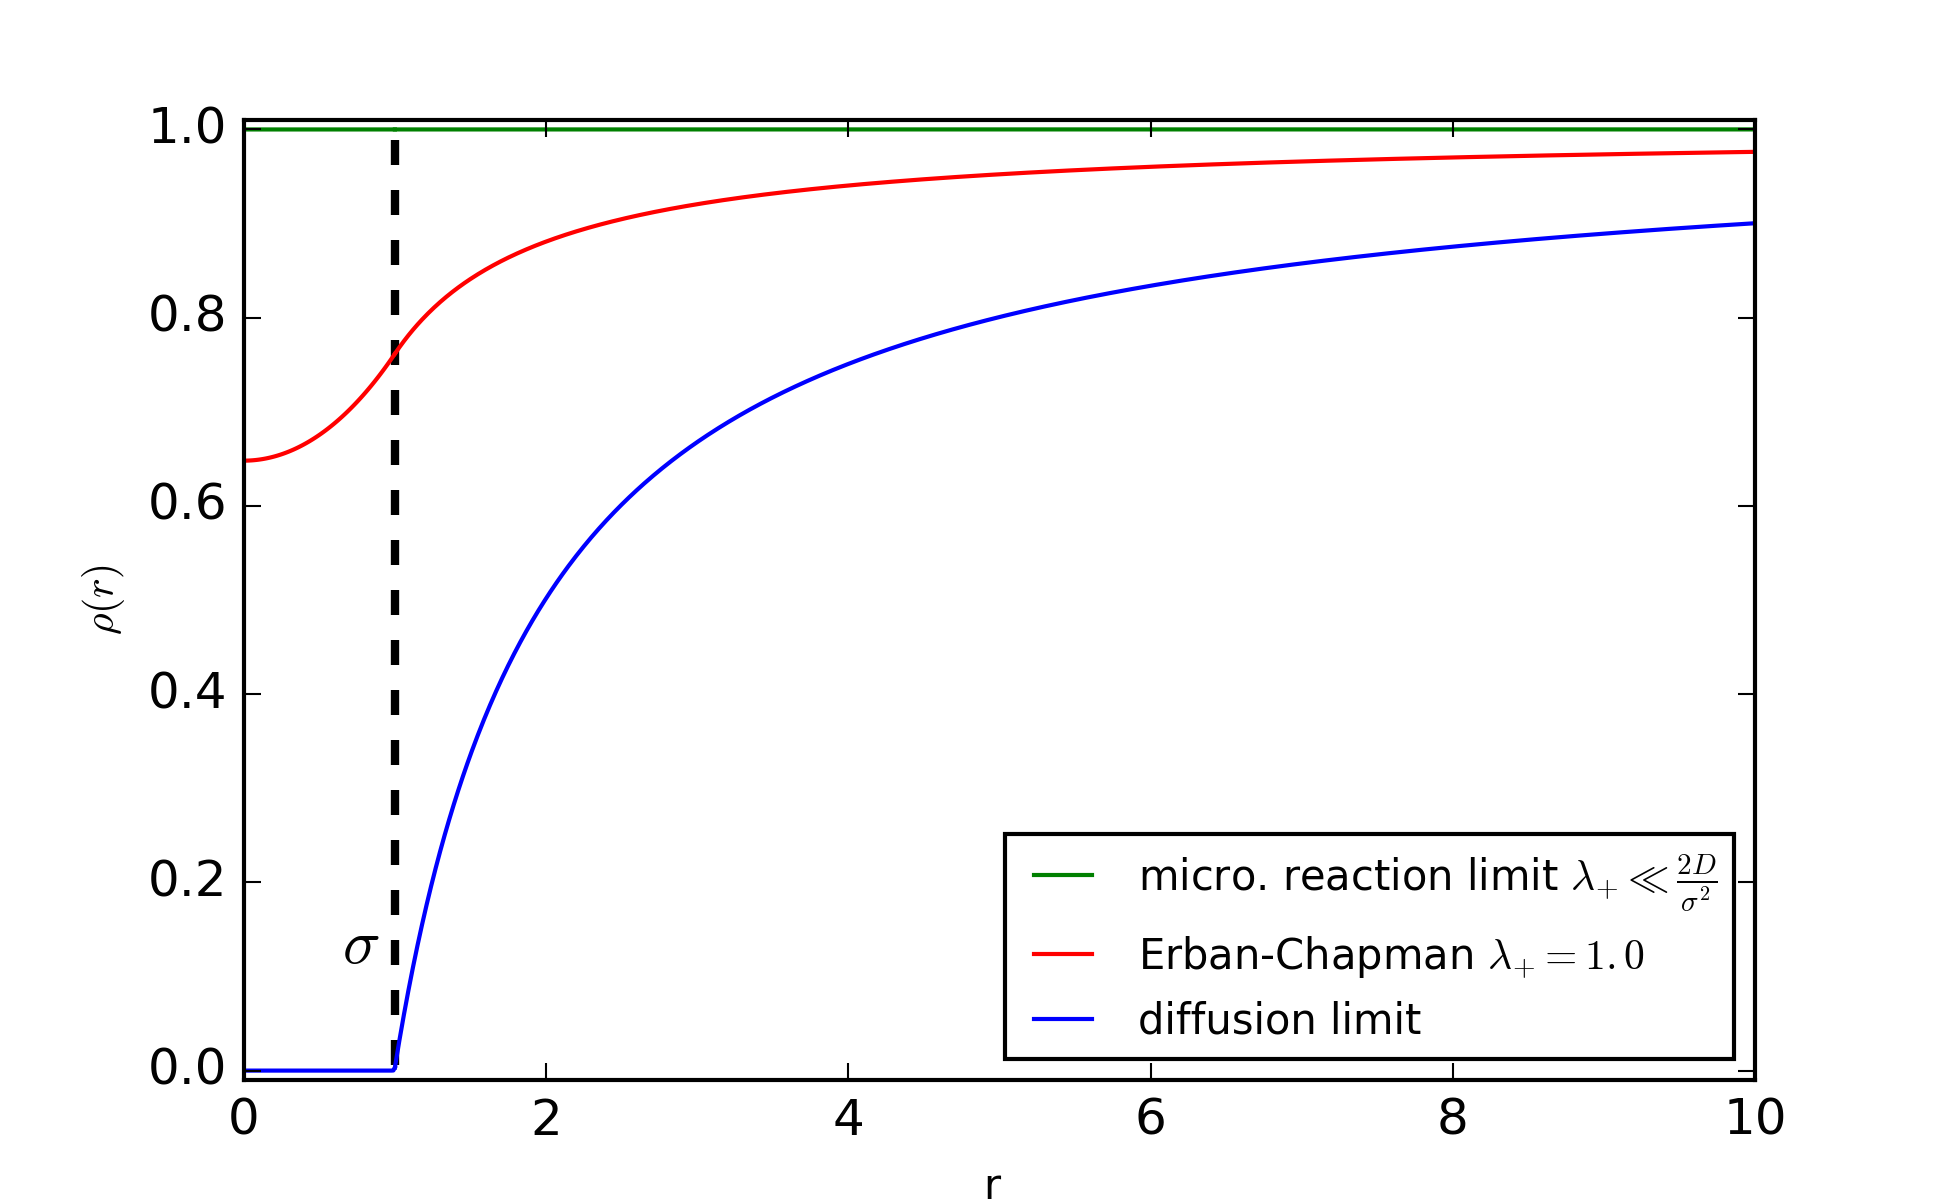
\includegraphics[width=\textwidth]{./data/smoluchowskierban.png}
  %\captionsetup{width=\linewidth}
\caption{Density distribution from \cref{erbanchapmanradial1,erbanchapmanradial} for a bi-molecular reaction from the Erban-Chapman derivation for three scenarios:}
\begin{enumerate}
  \item The microscopic reaction limit for $\lambda_{+} =0.0$ displayed as a green solid line
  \item An intermediate scenario with $\lambda_{+} =2d/\sigma^2$ displayed as a blue solid line.
  \item Smoluchwski's result for diffusion limited reactions   $\lambda_{+}=\infty $.
\end{enumerate}
  \label{fig:diffusion_limit-Erban-Chapmann-figure}
\end{figure}
\par
For the generalised problem with a microscopic rate $\lambda_{+}$ a diffusion and microscopic reaction limit can be shown. For $\lambda_{+} \rightarrow \infty $ reaction occur immediately and the diffusion limit is reached. If  $\lambda_{+} \ll \frac{D}{\sigma^2}$ a Taylor expansion of the Tangens Hyperbolicus in \cref{kalphaerbanchepmann} is given by:
\begin{align}
\tanh{x\rightarrow 0} \approx x-\frac{x^3}{3}
\end{align}
and \cref{kalphaerbanchepmann} can be written approximated as:
\begin{align}
 k_{+}=\frac{4 \pi \sigma^3 \lambda_{+}}{3}
\end{align}
The macroscopic reaction rate no longer depends on the diffusion but solely on the microscopic reaction rate. The stationary distributions for both limits and an intermediate scenario are plotted in \cref{fig:diffusion_limit-Erban-Chapmann-figure}.\par
The previous elaborations show that macroscopic reaction rates dependent on diffusion for bi-molecular reactions. For simple reaction diffusion systems the evolution and the stationary distribution of the density distribution can be obtained by solving Smoluchwoski's equation (PDE). For the bi-molecular reaction the law of mass action could be seen to follow for spatial homogeneity. Then reaction kinetics can be described for easy systems in terms of ODEs. Nevertheless complex systems cannot be solved. Further, for small molecular abundances of some chemical species deterministic models get inaccurate or even inapplicable. Stochastic models are necessary. Via chemical master equations (CMEs) and reaction diffusion master equations (RDMEs) analytical stochastic results can be obtained. Deduced from the Master equation also stochastic simulations based on Monte Carlo methods, like the prominent Gillispie algorithm \cite{Gillespie1977}, can be performed. This chapter however aims to introduce PBRD. The implementation of a PBRD simulation introduced in the next section follows the theoretical description of reactions with microscopic reaction rates within a reaction radius in this section.
% 
% 
% 
% Ab hier überleitung zu dann zur onvection-diffusion equation als motivation für simulations (ODE,PDEs, CME, RDME, PBRD, fractional PBRD). Letzteres analytic solution nicht einfach Fractional calculus, fractional Fokker-plank, frachtional master equation.
% 
% 
% 
% 
% 
% 
% 
% 
% It can also be interpreted as the production term in the continuity equation. In literature this equation is referred to as the convection-diffusion equation:
% \begin{align}
%  \frac{\partial \rho_t(r)}{\partial t}=-\left(\frac{\partial}{\partial_r}+\frac{2}{r} \right) j_t(r) + R \label{convenctiondiffsuion}
% \end{align}
% with $R$ the production term. For simple systems analytical solutions for theses partial derivative eqaution (PDEs) exist. 
% 
% 
% For easy problems analytical solutions to spatial distribution can be obtained by solving the convection diffusion \cref{convenctiondiffsuion}. \newline
% 
% 


% A particle based model for diffusion is Brownian motion introduced in the first chapter. Thereby similar to the setup of the previous elaborations by Erban and Chapman  particles can react within a certain distance $\sigma$ with a certain microscopic reaction rate $\lambda$. These calculation most 
% 
% Determinitic:
% Then Smoluchowski. (then gas theory wiki, maybe aurilius and kramers problem and simulations of proteins for determination of rates in reaction). back mass conservation with  production term. Then erban chapman. Then no diffusion (or diffusion time independ (and in-cooperated in marcoscopic rate.)). constant concentration (again mass action from gas theory)  . concentration  based models (ODEs) and solving . Then CME Then compartment based CME. 
% 
% Then stochastic simulations, stochstic cme. stochstic compatment based cme. stochastic particle based simulations smoluchawoski/diffsuion equation to Fockerplank. (fluctuations / dissipation ) theorem.
% 
%  
% 
% 
% 
% 
% 
% 
% Deterministic models have their origin.  
% 
% 
% stationary values. kinetics. spatial distribution of reactants. 
% 
% What are interesting observables. Solutions in dynamical equilibrium reaction rates rate equtaions ( assumption rate is independent of time. not nesesarilly true.  chemical equlubrium. Mass action. order of reaction. Smoluchowski. Chemical master equation. quantum physical -> bonds between reactants for example electrons involved.
% \section{chemical reactions}
% With no information on 
% The classical theory of reaction 
%  
% 
% 
% 
% 
% 
% 
% 
% In biological systems, phenomena often depend on stochastic fluctuations. Deterministic models often are often inaccurate or even not applicable at all. 
% (von franks Vortrag das Bild mit den unterschiedlichen Methoden zur genererieung von Reactiondiffusions systemen). 
% This chapter is going to discuss particle based reaction diffusion. Particle based reaction diffusion is going to be put in relation to different reaction diffusion studying methods.  
% Analytical solutions for resulting ordinary differencial equation exist under certain conditions like Quasi-Steady-State assumption or equilibrium assumption. In any case the mass action law is assumed. For fractional diffusion mass action law does not apply. Thus concentration based models had been upgraded by time depended rate coefficients \cite{Berry2002}  \cite{schnell2004reaction}
% \section{Smoluchowski}
% \section{Erban Chapmann}
\section{RevReaddy with fBm} 
RevReaDDy is a PBRD tool developed by Christoph Fröhner whithin his PHD project under supervision of Frank Noé. It is not published. Many modification to the tool had to be done in the process of this thesis. ReRreaDDy is based on the simulation package ReaDDy by Johannes Schöneberg and Frank Noé \cite{10.1371/journal.pone.0074261}. Reaction-diffusion dynamics of all particles can be resolved in space and time. Particles are modelled as spheres with possible particle interaction potentials. The tool aims to bridge the gap between molecular simulation and CME/RDME simulations. It is written in C++. However, the user can setup up and simulate the desired reaction scheme in Python via a Python binding. Particle types with a specific radius and diffusion constant can be defined. Particles of a predefined particle type can be placed anywhere into a simulation box with variable box size and periodic boundary conditions. A desired simulation length and width of the time step have to be set. Conventionally particles propagate by Brownian Dynamics. In the process of the thesis also a fractional Brownian motion integrator with the circulant method by Davis-Harte \cite{Dieker2004}  and Lowen \cite{Lowen1999} was implemented. For Brownian Dynamics, potentials with two different potential types, Lennard Jones and soft repulsion, can be introduced to act in-between participles and between fixed geometries in the simulation box and particles. Thereby a temperature has to by defined. Particles can be e.g limited to diffuse on a surface by a potential. It can be chosen from various reaction types to affect the particle types. For uni-molecular reactions like conversion \ch{A <=>[ $k$ ][ $k'$ ] B}, annihilation \ch{A -> [ $k$ ] $\emptyset$}, decay \ch{$A$ ->[ $k$ ] $B+C$} the probability that one particle undergoes a reaction within the $\Delta t$ is simply approximated as:
\begin{align} \label{propabilityreaction}
 P(n)=1- \exp[-\lambda \Delta t n] \approx \lambda \Delta t n \qquad \text{for} \qquad P(1)\ll 1
\end{align}
Here $n=t/\Delta t$. A more sophisticated algorithm, which draws the reaction time from the correct distribution is the Gillispie algorithm \cite{Gillespie1977}. It could by implemented into RevReaDDy as a improvement. Microscopic reaction rates $\lambda$ for such reactions are independent of the position.
\begin{figure} 
  \centering
  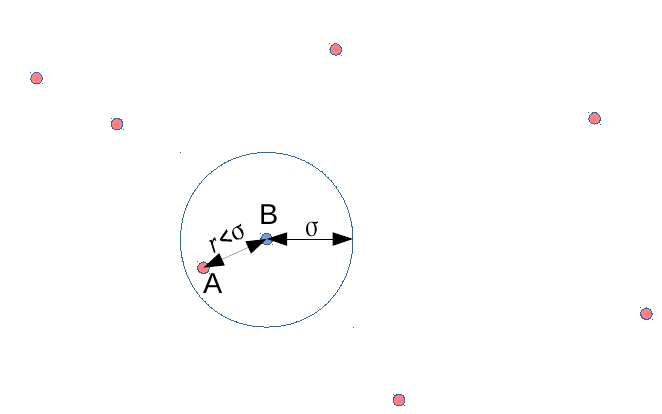
\includegraphics[width=0.7 \textwidth]{./data/schemeforreacions1.png}
  \captionsetup{width=\linewidth}
  \captionof{figure}{The Figure shows a visualisation of a bi-molecular reaction between particle A and B in RevReaDDy. Particle B are coloured blue and particle A are coloured red. }
  \label{fig:model-reactions}
\end{figure}
\par
For the decay reaction a weighting factor and reaction distance shall be defined. They determine how far each of the particles are placed from the previously existing complex. With waiting factor equals zero particle A is placed at the position of the pre-existing complex and particle B is placed with the a uniform distribution in the sphere with reaction radius $\sigma$. For bi-molecular reactions like the enzymatic reaction with complex building \ch{$A + B$ <=>[ $k$ ][ $k'$ ] $A + C$} or fusion \ch{$A + B$ ->[$k$] C} relative positions of the reactants are important for the reaction to take place. Analogous to the setup up of Erban and Chapman in \cref{Erban-chapman-section} a microscopic reaction rate $\lambda$ within a reaction distance $\sigma$ have to be defined. If the reactants come closer than $\sigma$ a reaction takes place with probability $P= \lambda \Delta t$. The problem is visualised in \cref{fig:model-reactions}. Thereby the time step cannot by chosen arbitrarily large. The mean square displacement for Brownian motion in three dimensions is given as $\delta r^2(\Delta t)= 6D \Delta t$. The mean displacement during one time step has to be a lot smaller then the squared penetration length $\delta r^2(\Delta t)\ll 1/\kappa^2$ . Otherwise differences between the time of particles staying within a radius $\sigma$ to another particle would differ significantly in comparison to $\Delta t \rightarrow 0$. Thus, also the macroscopic reaction rates would become less accurate. For fractional Brownian motion with $\alpha<1$ and the effect increases. A variety of observables are provided in RevReaddy, which are written into HDF5 files \cite{hdf5} during the simulation. Possible observables are: Acceptance rate, energy, mean square displacement, particle number, radial distribution functions, amount of reactions, increments and positions. Observables can mostly be defined to consider any particle type over any period in time. 

\chapter{An Enzymatic Reaction With Fractional Brownian Motion}
Enzymes are large biological molecules mostly proteins. They have a key role especially in metabolic processes in cells. They help to break down large nutrient molecules like carbohydrates, fats and proteins during in the process of digestion. Other enzymes contrariwise help forming large and complex molecules from smaller once. Enzymes are involved in storage and release of energy, processes of respiration, vision, muscle contraction, transmission of nerve impulses. In fact biochemical reactions are controlled mainly by enzymes. In general they act as catalysts by lowering the activation energy. As stated by the Arrhenius law the activation energy is then increasing the reaction rates. The speed of reactions is typically increased by $10^6-10^{14}$. So reactions with enzymes involved take place a lot faster than without. Enzymes do not change the equilibrium concentrations. Enzymes are mostly proteins. They have a defined amino acid sequence and a three-dimensional structure. The specific three-dimensional structure contains an active side for a substrate molecule to bind and orient and a catalytic site to reduce the chemical activation energy. Usually, an enzyme molecule has only one active site, and the active site fits with one specific type of substrate. So enzymes mostly have a high specificity for a particular type of reaction. Catalysis follows the binding of the substrate to the binding side. Some residues can be both, part of the binding side and catalytic site. The catalytic site lowers the activation energy for the reaction. After reaction takes place the product is released. The enzyme is free to start the reaction with a new substrate. From a single enzyme and single substrate to a single enzyme and single product many reversible intermediate states can be present in the reaction mechanism. A simple representation of the mechanism with two complex intermediate states can be written as:
\begin{align} \label{eq:enyzmescheme}
\ch{S + E <=>[$ k_1 $][$ k'_1 $] ES <=> [$ k_2 $][$ k'_2 $]EP<=>[ $k_3 $][$ k'_3 $]P + E}
\end{align}
$k$ are the forward rates and $k'$ the backward rates. $\mathrm{S}$ and $\mathrm{P}$ are substrates and products, respectively. $\mathrm{ES}$ and $\mathrm{EP}$ are intermediate complexes. By the law of mass action ODEs can be formulated but not solved.\par
The focus of this chapter is to study the kinetics and spatial distribution of the Michaelis-Menten mechanism, an even simpler mechanism, without and with fractional Brownian motion. Some related theoretical work on the fractional reaction diffusion equation of the Michaelis-Menten mechanism had been done by Abdullah \cite{AiniAbdullah2011}. Monte Carlo simulations with the anomalous diffusion modeled by a random walk and immobile obstacles were performed by Berry and Schnell \cite{Berry2002, Schnell2004}. An overview on stochastic modeling of in vivo reactions was given by Turner \cite{Turner2004}. Recently first passage time simulations with fBm  were performed by Jae-Hyung Jeon, A. V. Chechkin and Ralf Metzler \cite{Jeon2014}. Nevertheless, a Michaelis Menten mechanism with fractional Brownian motion was not yet studied.
\section{Michaelis-Menten (MM) kinetics}
Leonor Michaelis and Maud Menten  proposed in 1913 a mathematical model for enzyme kinetics. Their most important contribution was to assume an enzyme-substrate to be present \cite{michaelis1913kinetik}. In their honor it is also called Michaelis-Menten complex. A simpler version of \cref{eq:enyzmescheme} was proposed as the Michaelis-Menten mechanism:
\begin{align} \label{eq:michaelismechanism}
\ch{S + E <=>[$ k_+ $][$ k_- $] ES -> [ $k_c $]P + E}
\end{align}
 The rate of the backward reaction from products and enzymes to  complexes was assumed to be negligible. They postulated the relation between the reaction velocity, formation of products, and the concentration of substrates. This relation is captured by the so called Michaelis-Menten equation:
\begin{align} \label{michaelis-menten-equation}
 v=\frac{v_{max} c_s}{K_M+ c_s}
\end{align}
$v_{max}$ is the maximum reaction velocity. The Michaelis constant $K_M$ is the substrate concentration with $50 \%$ of maximum velocity and $c_s$  is the concentration of the substrate. A derivation of the Michaelis-Menten equation was done by Briggs and Haldane in 1925 assuming the mass action law, mass conservation and a quasi-steady state approximation (QSSA). It states that after a negligible initial transition period ($t>t_c$) the concentration of the complex vary slowly as if in a quasi-steady state $dC_{ES}/dt=0$. The approximation was shown to hold for $c_{E_0}\ll K_M \text{ or } K_M \ll c_{S_0}$ \cite{Palsson1987}. A derivation of \cref{michaelis-menten-equation} can be found in the Appendix \ref{Menten_der}. In 1997 a closed form for the kinetics of the Michaelis-Menten mechanism with the quasi-steady state approximation was derived by Schnell amd C.Mendoza \cite{Schnell1997}:
\begin{align}
 c_S(t)&=K_M \mathrm{W}\left(\frac{c_{S_0}}{K_M} \exp \left( \frac{-v_{max} t + c_{S_0}}{K_M}\right)\right)  \label{tiemdependedC_S} \\
 c_{ES}(t)&= \frac{c_{E_0} c_S(t)}{K_M+c_S(t)} (1- \exp(-(K_M + c_S(t) k_+))\label{timedendendces}\\ 
 c_{E}(t)&=c_{E_0}(t)-c_{ES}(t) \label{timedendendce}\\
 c_{P}(t)&=c_{S_0}-c_S(t)+c_{ES}(t) \label{timedendendcp}
\end{align}
$v_{max}=k_2 c_{E_0}$ is the maximum velocity,  $\mathrm{W(x)}$ is the omega function and the Michaelis-Menten constant is defined as:
\begin{align}
 K_M= \frac{k_{-}+k_c}{k_+}
\end{align}
The quasi-steady state approximation was applied in the derivation of $c_S(t)$. A time independent $c_{ES}$ is conventionally solved for the transitions period $t<t_c$ by approximating $c_S(t<t_c) \approx c_{S_0}$. For \cref{timedendendces} the result for the time independent $c_{ES}$ during the transitions period ($t<t_c$) was extended to the total period of time ($0<t<\infty$) by applying time depended $c_S(t)$ from \cref{tiemdependedC_S}. For normal diffusion theses equation will be used to fit the concentrations resulting from the simulation.  Still for a small number of particles deterministic approach may differ from the averages of the stochastic simulation \cite{Turner2004}.\par
The quasi equilibrium approximation is the second very common approximation typically applied on setups with high enzyme concentrations. It is assumed that the binding step quickly reaches an equilibrium state ($c_S c_E/c_{ES}=K_S$). $K_S=k_-/k_+$ is the dissociation constant and the rate of product formation can be written as:
\begin{align}
 v={\frac{V_{max} c_S}{K_S+ c_S}}
\end{align}
The assumption was shown to be true for $c_{E_0}\gg K_M \text{ or } k_- \gg k_c$.  \cite{Palsson1987}.\par A description of the Michaelis Menten mechansim with fractional Brownian motion by fractional fractional diffusion reaction equation \cite{Yuste2002} was done by Abdullah \cite{AiniAbdullah2011}. An earlier description of reaction kinetics with fractional diffusion was done by Kopelman \cite{Kopelman1988} for a percolation cluster with a scaling theory and an upgraded time depended reaction rates. This concepts were applied by Berry \cite{Berry2002} and Schnell \cite{Schnell2004} for the Michaelis Menten mechanism.
\section{Simulation Model}
The simulation of the Michaelis-Menten mechanism \cref{eq:michaelismechanism} and fractional Brownian motion with the circulant method by Davis-Harte \cite{Dieker2004} was setup up with RevReaDDy. Four particle types were defined: substrate, product complex and enzyme. Substrates and products were set to diffuse with the general diffusion constant $K_{\alpha}=1/6 $. Enzymes and complexes are modeled to be immobile with $K_{\alpha}=0$. Enzymes are often even 100 times heavier than substrates or products and therefore diffuse a lot slower.  A single enzyme was set in the origin $(x,y)=(0,0)$ and 20 substrates were placed randomly in the simulation box with the box size $l$ and periodic boundary conditions. Two association/decay reaction types were defined:  \ch{S + E <=>[$ k_+ $][$ k_- $] ES} and \ch{P + E <-[$ k_c $] ES} with intrinsic reaction rates $\lambda_+$,$\lambda_-$ and $\lambda_c$ for complex formation, decay into substrate and enzyme and decay into product and enzyme, respectively. The reaction radius $\sigma $ was set for both reaction types to be $1$. A desired simulation length $M=2^{14}$ and length of the time step $\Delta t=0.05$ was set. $1/\kappa= \sqrt{\lambda_+/D}$ can be defined as the penetration length into the the reaction square. Reaction distance should be larger than the mean displacement traveled with one step. Otherwise the time of one particle staying within the reaction radius and thus the reaction rate would have large errors due to finite time step errors. In this simulation setup with $\sigma =1 $ and $\Delta t=0.05$  and regardless of $\alpha$ the particles on average travel for $n=20$ steps $\sqrt{6K_{\alpha} n \Delta t^{\alpha}} \sigma$ to overcome the distance $\sigma$. Further the reaction probability  as approximated in \cref{propabilityreaction} should be a lot smaller than  $P(\Delta t)=\lambda \Delta t \ll 1$. Otherwise that approximations fails to describe the correct reaction probability $P(t)=1-\exp(-\lambda t)$. Simulations for various $\lambda_+$ ,$\lambda_-$,$\lambda_c$, box size $l$ and $\alpha$ were performed. The results are discussed in the next two sections.
\section{Results for Normal Diffusion}
First simulations with normal diffusion were set up to have a connection to the results from the Smoluchowski and Erban-Chapman problem. The difference in kinetics of the Michaelis Menten mechanism to the Erban-Chapman problem is a possible blocking of the enzyme. Thus slowing down the reaction speed and a higher local concentration of the substrates in close proximity to the enzyme because of the back reaction. At first  a reaction similar to the Erban-Chapman problem was aimed to simulate. Therefore  $\lambda_-=0$  was chosen to neglect the effect of a higher local concentration of substrates and $\lambda_+>\lambda_c$ to neglect enzyme blocking. Thereafter the normal MM mechanism was studied. 
\subsection{Results for one Way Reactions}
\begin{figure}
  \centering
  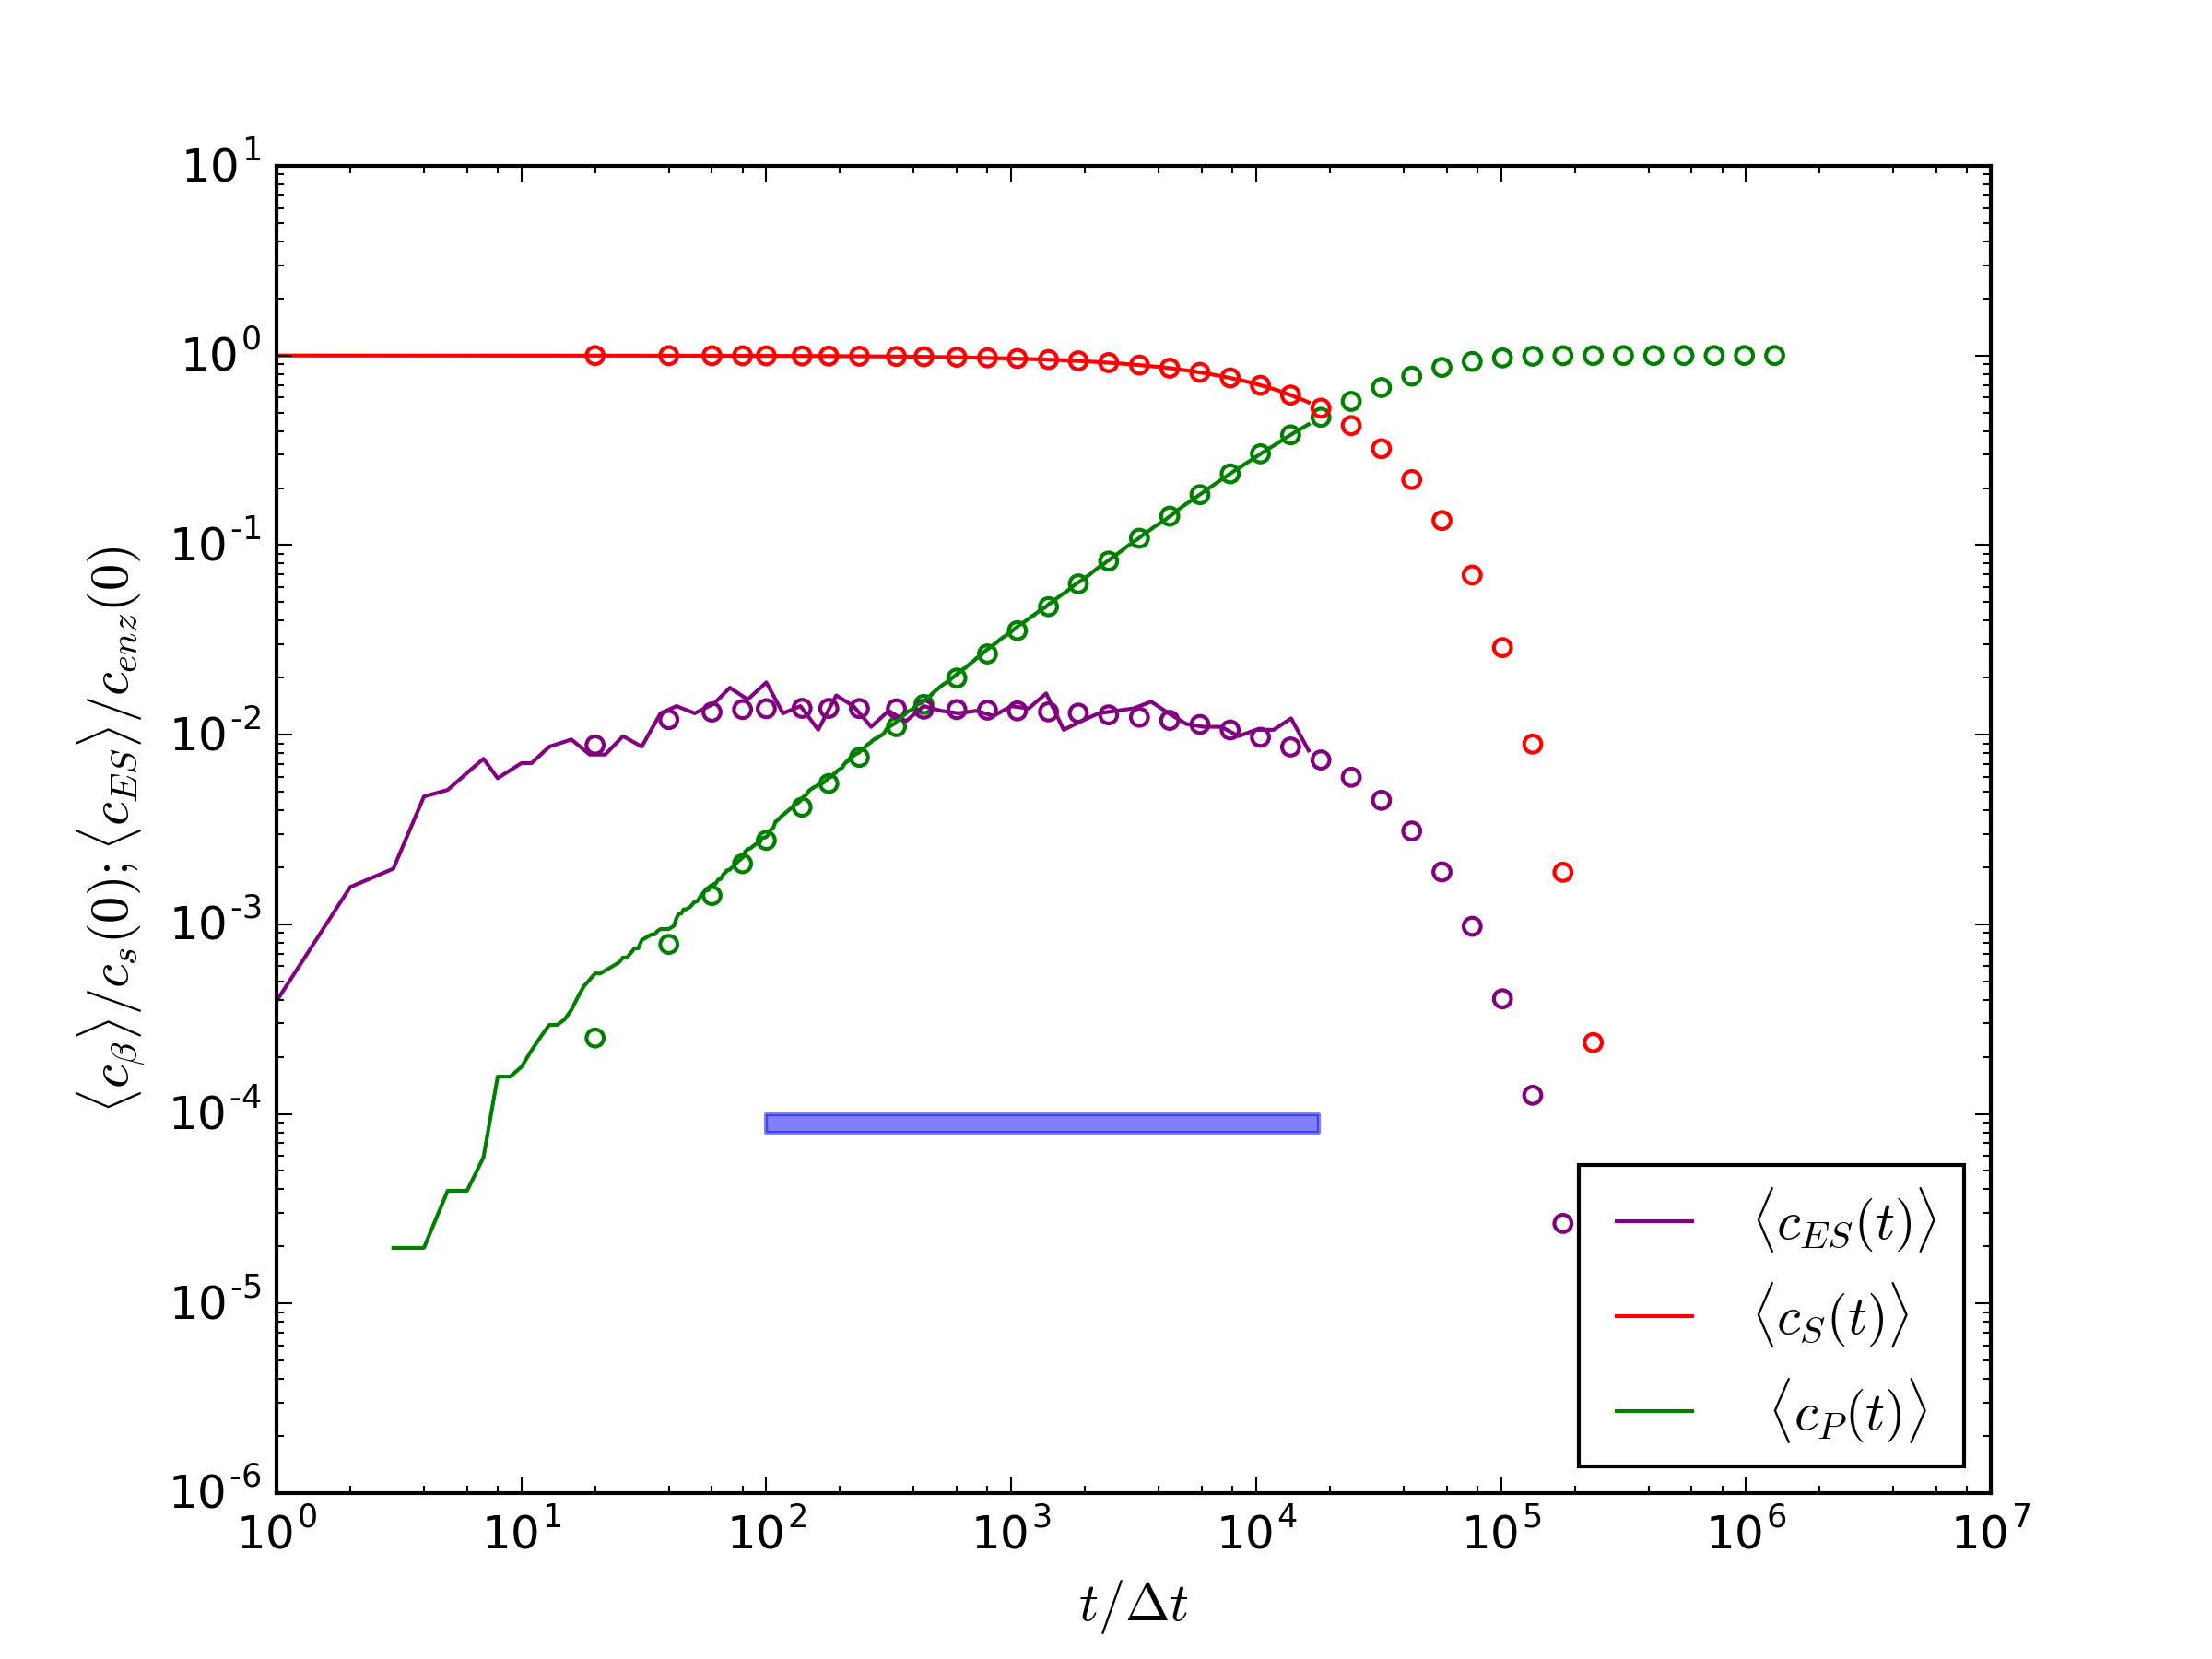
\includegraphics[width=\textwidth]{./data/chapman-limit-concentrations1.png}
  \captionsetup{width=\linewidth}
  \captionof{figure}{ Normalized concentrations of substrate, product and complex and their fit with the quasi-steady state approximation for the substrate concentration are shown in the loglog plot. The blue bar in the plot indicates the area where the radial distribution was observed, which is plotted in \cref{fig:diffusion_limit-Erban-Chapmann_radial}. Parameters were set to:  $\lambda_+=0.1$, $\lambda_-=0$,  $\lambda_c=1.0$ and the box size $l^3=8^3$.}
  \label{fig:diffusion_limit-Erban-Chapmann}
\end{figure}
\begin{figure}
  \centering
  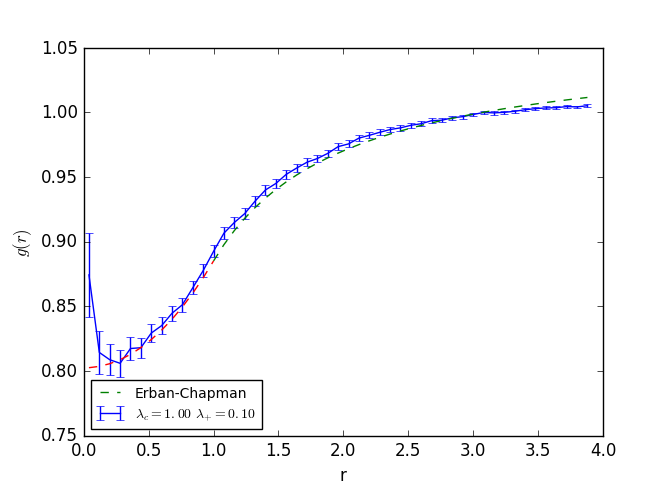
\includegraphics[width=\textwidth]{./data/chapman-limit-radial.png}
  \captionsetup{width=\linewidth}
  \captionof{figure}{The radial distribution function of the substrates around the enzyme / complex was observed for $5<t<900$ and plotted as a blue line with an error-bar of the standard deviation. The Erban-Chapman result was plotted as a green dashed line for bigger than the reaction radius $\sigma$  and a red dashed line for smaller than $\sigma$. Parameters were set to:  $\lambda_+=0.1$, $\lambda_-=0$,  $\lambda_c=1.0$ and the box size $l^3=8^3$.}
  \label{fig:diffusion_limit-Erban-Chapmann_radial}
\end{figure}

\begin{figure}
  \centering
  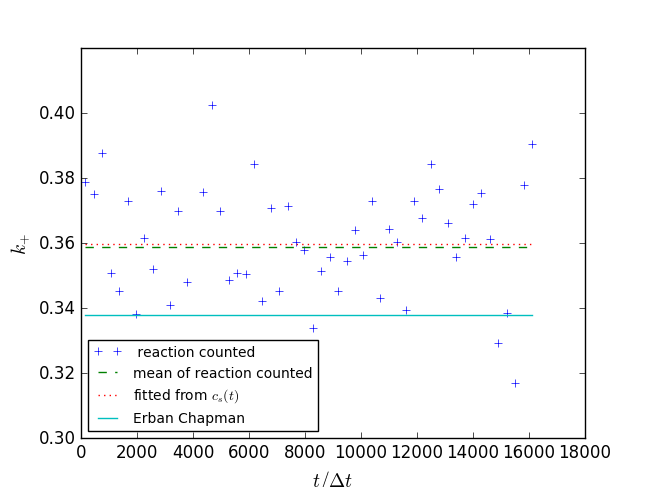
\includegraphics[width=\textwidth]{./data/chapman-limit-concentrations1_k1.png}
  \captionsetup{width=\linewidth}
  \captionof{figure}{ A comparison of $k_+$ from three different calculations. $k_+$ was calculated from the number of reactions with \cref{reactioncount} and marked as blue crosses. The Mean of this $k_+$ is plotted as a green dashed line. The result for $k_+$ from the fit of the substrate concentration \cref{tiemdependedC_S} with the QSSA is plotted as a red dotted line and the result form the Erban-Chapman \cref{kalphaerbanchepmann} problem is plotted as a solid cyan colored line. Parameters were set to:  $\lambda_+=0.1$, $\lambda_-=0$,  $\lambda_+=1.0$ and the box size $l^3=8^3$.}
  \label{fig:diffusion_limit-Erban-Chapmann_k1}
\end{figure}
The first simulations was performed under normal diffusion $\alpha=1$ and with $\lambda_-=0$  in a simulation box of size $l^3=8^3$ . The reaction mechanism results in:
\begin{align} \label{eq:michaelismechanismneu}
\ch{S + E ->[$ k_+ $] ES -> [ $k_c $]P + E}
\end{align}
$\lambda_+=0.1$ was set to be the rate limiting step in the reaction chain and $\lambda_c=1.0$ was set to reproduce approximately the Erban-Chapman problem.
The average normalized number of substrates $c_{S}(t)/c_{S_0}$, the normalized number of products $c_{P}(t)/c_{S_0}$ and the averaged number of complexes $c_{ES}(t)$  (over $2544$ runs) were observed and visualized in a loglog plot in \cref{fig:diffusion_limit-Erban-Chapmann}. Every run had a new random (uniformly distributed) initial position of the substrate molecules. The simulated concentrations are shown as solid lines. The curves were fitted to obtain $k_+$ with the quasi-steady state approximation from \cref{tiemdependedC_S}. The microscopic reaction rates and macroscopic reaction rate for a uni-molecular reaction should be similar $\lambda_c=k_c$.  With all macroscopic rates available, the MM kinetics with the quasi-steady state approximation for the substrate were plotted from \cref{tiemdependedC_S,timedendendces,timedendendce,timedendendcp} as dashed lines in \cref{fig:diffusion_limit-Erban-Chapmann}. A blue bar in the plot indicates the time during which the radial distribution was observed. It was assumed that after 20 steps a stationary distribution was reached. The assumption was based on an approximated constant average number of complexes from there on. The radial distribution of the substrates around the enzyme/complex from 0 to the boundary of the simulation box $0<r<4.0$ was plotted in \cref{fig:diffusion_limit-Erban-Chapmann_radial}. It was obtained by averaging over a normalized histogram of substrate particles. The Erban-Chapman solution \cref{erbanchapmanradial1,erbanchapmanradial} was plotted with dashed lines. The Erban-Chapman radial distribution is reproducing with good accuracy the observed radial distribution obtained by averaging over the histograms. For a better agreement substrate particles should be placed at the boundaries during the simulation to get a stationary concentration. The macroscopic reaction rate  $k_+$ was calculated from the number of reactions $N_{reaction}$ of the reaction \ch{S + E <=>[$ k_+ $] ES}. $k_+$ can be calculated from the reaction number change as:
 \begin{align} \label{reactioncount}
  k_+=\frac{d N_{reaction}}{dt}\frac{1}{V c_S c_E} 
 \end{align}
$V$ is the volume of the simulation box. Numerically the difference of the average reaction number was calculate. $k_+$ was very noise. It could be smoothed by averaging over 300 time steps. The result was plotted in \cref{fig:diffusion_limit-Erban-Chapmann_k1} as blue crosses. The average of these blue crosses was plotted as a dashed green line. The result for $k_+$ from the fit of the substrate concentration \cref{tiemdependedC_S} with the QSSA was plotted as a red dotted line and the result form the Erban-Chapman \cref{kalphaerbanchepmann} problem was plotted as a solid cyan colored line.\par
\begin{figure}
  \centering
  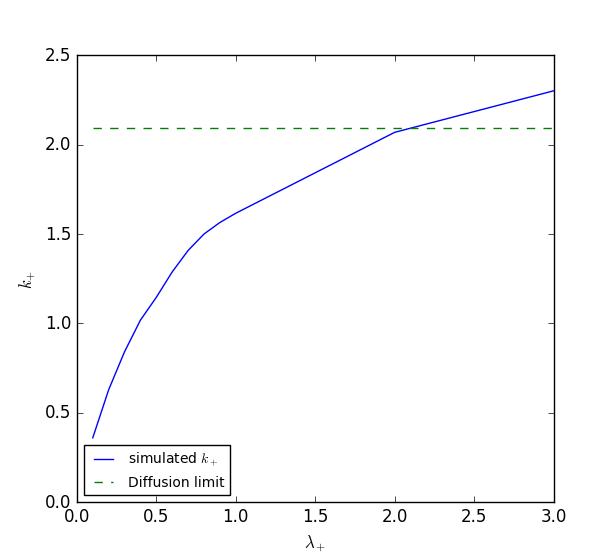
\includegraphics[width=\textwidth]{./data/diffusion-limit-concentrations1_k1.png}
  \captionsetup{width=\linewidth}
  \captionof{figure}{ Parameters were set to:  $\lambda_c=1.0$, $\lambda_-=0$ and the box size $l^3=8^3$. The blue solid line shows macroscopic rates $k_+$ in respect to  microscopic rate $1\leq\lambda_+\leq3.0$. The macroscopic rates are obtained with a fit of the substrate concentration \cref{tiemdependedC_S} with the QSSA. The diffusion limit \cref{difkinetics} is plotted as the dashed blue line.}
  \label{fig:diffusionlimit_k1}
\end{figure}
\begin{figure}
  \centering
  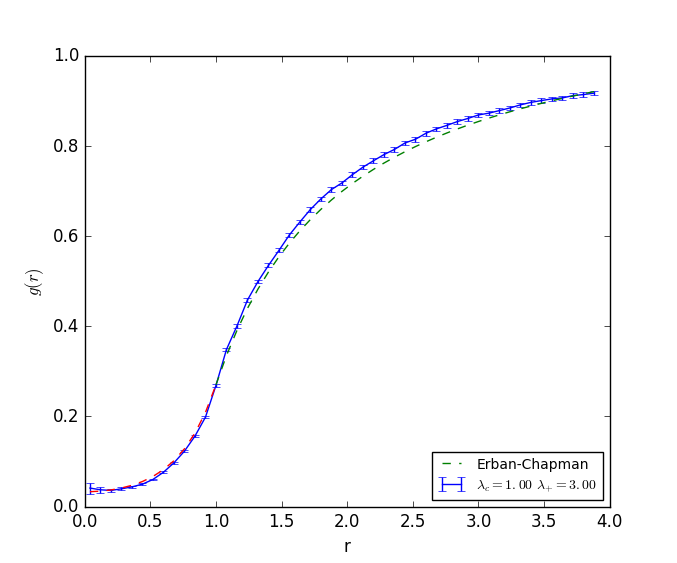
\includegraphics[width=\textwidth]{./data/limit-radial.png}
  \captionsetup{width=\linewidth}
  \captionof{figure}{The radial distribution function of the substrates around the enzyme / complex was observed for $5<t<900$ and plotted as a blue line with an error-bar of the standard deviation. The Erban-Chapman result was plotted as a green dashed line for bigger than the reaction radius $\sigma$  and a red dashed line for smaller than $\sigma$. Parameters were set to:  $\lambda_+=3.0$, $\lambda_-=0$,  $\lambda_c=3.0$ and the box size $l^3=8^3$.}
  \label{fig:diffusion1_limit-radial}
\end{figure}
On the other hand a setup were reaction kinetics are limited by diffusion was tried to setup. Therefore  $\lambda_c=1.0$, $\lambda_-=0$ and the box size $l^3=8^3$ were set fixed and  $1\leq\lambda_+\leq3.0$ scanned until diffusion becomes the rate limiting step. The macroscopic rates were obtained by fitting the substrate concentration with \cref{tiemdependedC_S}. The fastest possible reaction should be limited by \cref{difkinetics} to be $k_+=2.094$. Even higher reaction rates were observed for $\lambda_+=2.0 \text{ and }3.0$ possibly because no extra particles were placed at the boundaries to indeed have a quasi stationary distribution. The radial distribution function was again obtained by a histogram observed for $5<t<900$ and compared with good agreement to the Erban-Chapman result in \cref{fig:diffusion1_limit-radial}. Even for the closest scenario to reactions being limited by diffusion the quasi steady state approximation still should hold because of $0.002 \approx c_{E_0}\ll K_M\approx 0.04$  as stated by \cite{Palsson1987}. 
\begin{comment}
  

\begin{figure}
  \centering
  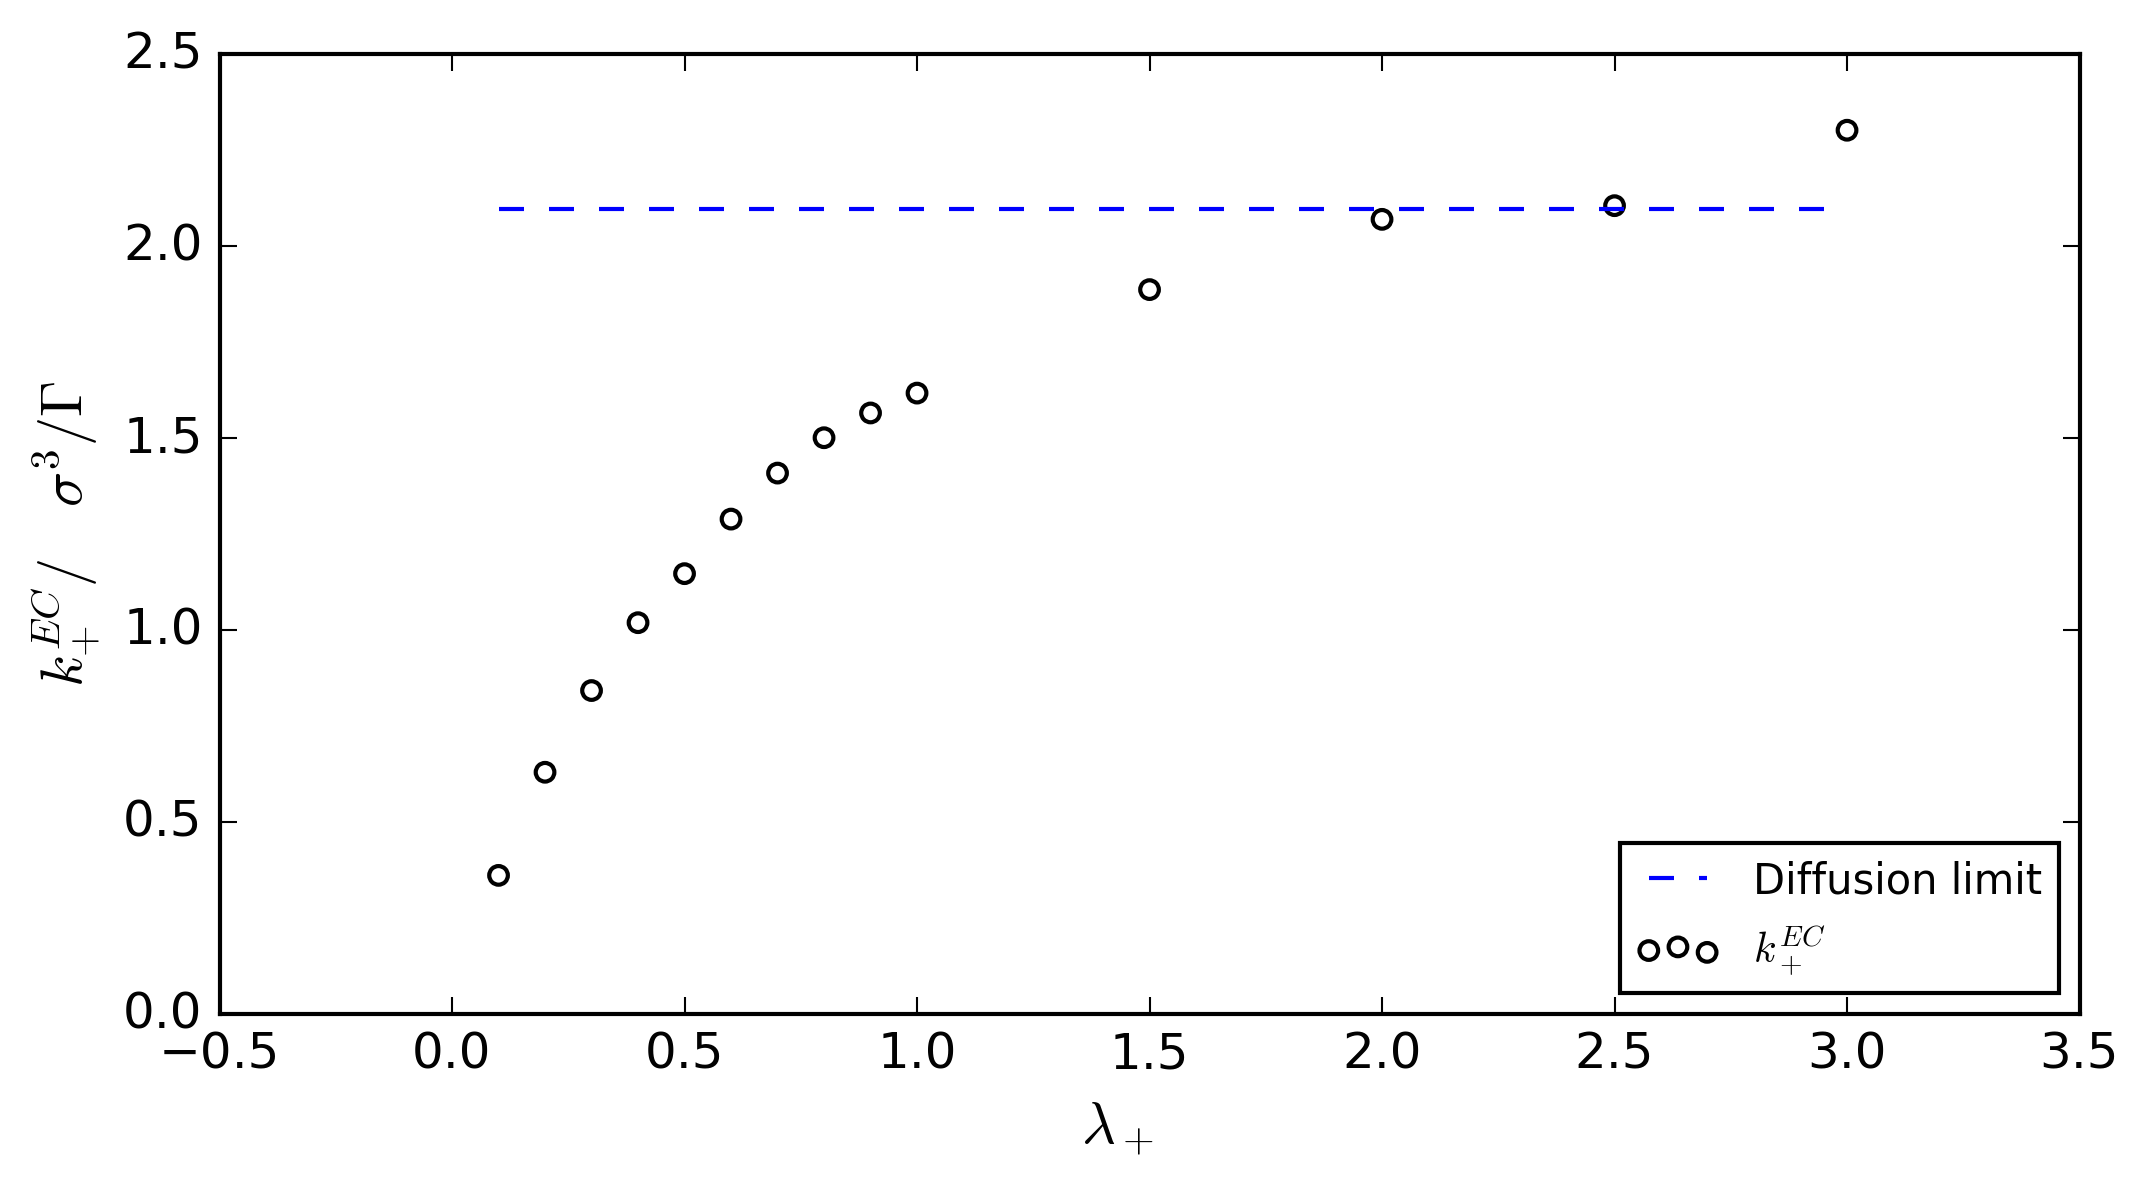
\includegraphics[width=\textwidth]{./data/diffusion-limit-concentractionlambdaminus_k1.png}
  \captionsetup{width=\linewidth}
  \captionof{figure}{ Parameters were set to:  $\lambda_c=1.0$,  and the box size $l^3=8^3$. The green solid line shows macroscopic rates $k_+$ in respect to  microscopic rate $1\leq\lambda_+\leq3.0$ for $\lambda_-=0$ and the blue solid line for $\lambda_-=1$. The macroscopic rates are obtained with a fit of the substrate concentration \cref{tiemdependedC_S} with the QSSA. The diffusion limit \cref{difkinetics} is plotted as the dashed blue line.}
  \label{fig:diffusionlimit_k1variouslambda}
\end{figure}
 \end{comment}
 \newpage
\subsection{Results for the MM mechanism}
The first scenario of the MM mechanism was $\lambda_{-}>\lambda_c$ and $\lambda_{+}>\lambda_c$ to have a local higher concentration of substrates around the enzyme. The radial distribution function was plotted in \cref{fig:diffusion1_limit-radial_local concentration} with the Erban-Chapman result as a reference. Determining $k_{+fit}=4.34$ from the fit of \cref{tiemdependedC_S} results in a lot higher reaction rate than the Erban Chapman result $k_{+erban}=1.25$. It is the result of the high local concentration of substrates around the enzyme. \cref{tiemdependedC_S} however, is based on the mass action law with homogeneously distributed substrates. The fits from the quasi steady state approximation  with $k_{+fit}$ and the average and not local concentration are still in well agreement with the data from the simulation. This can be seen in x-log plot in \cref{fig:enzyme_blocking}. Also the method of counting reactions \cref{reactioncount} is based on an average concentration and results in similar macroscopic reaction rate $k_{+count}=4.39$. 
\begin{figure}
  \centering
  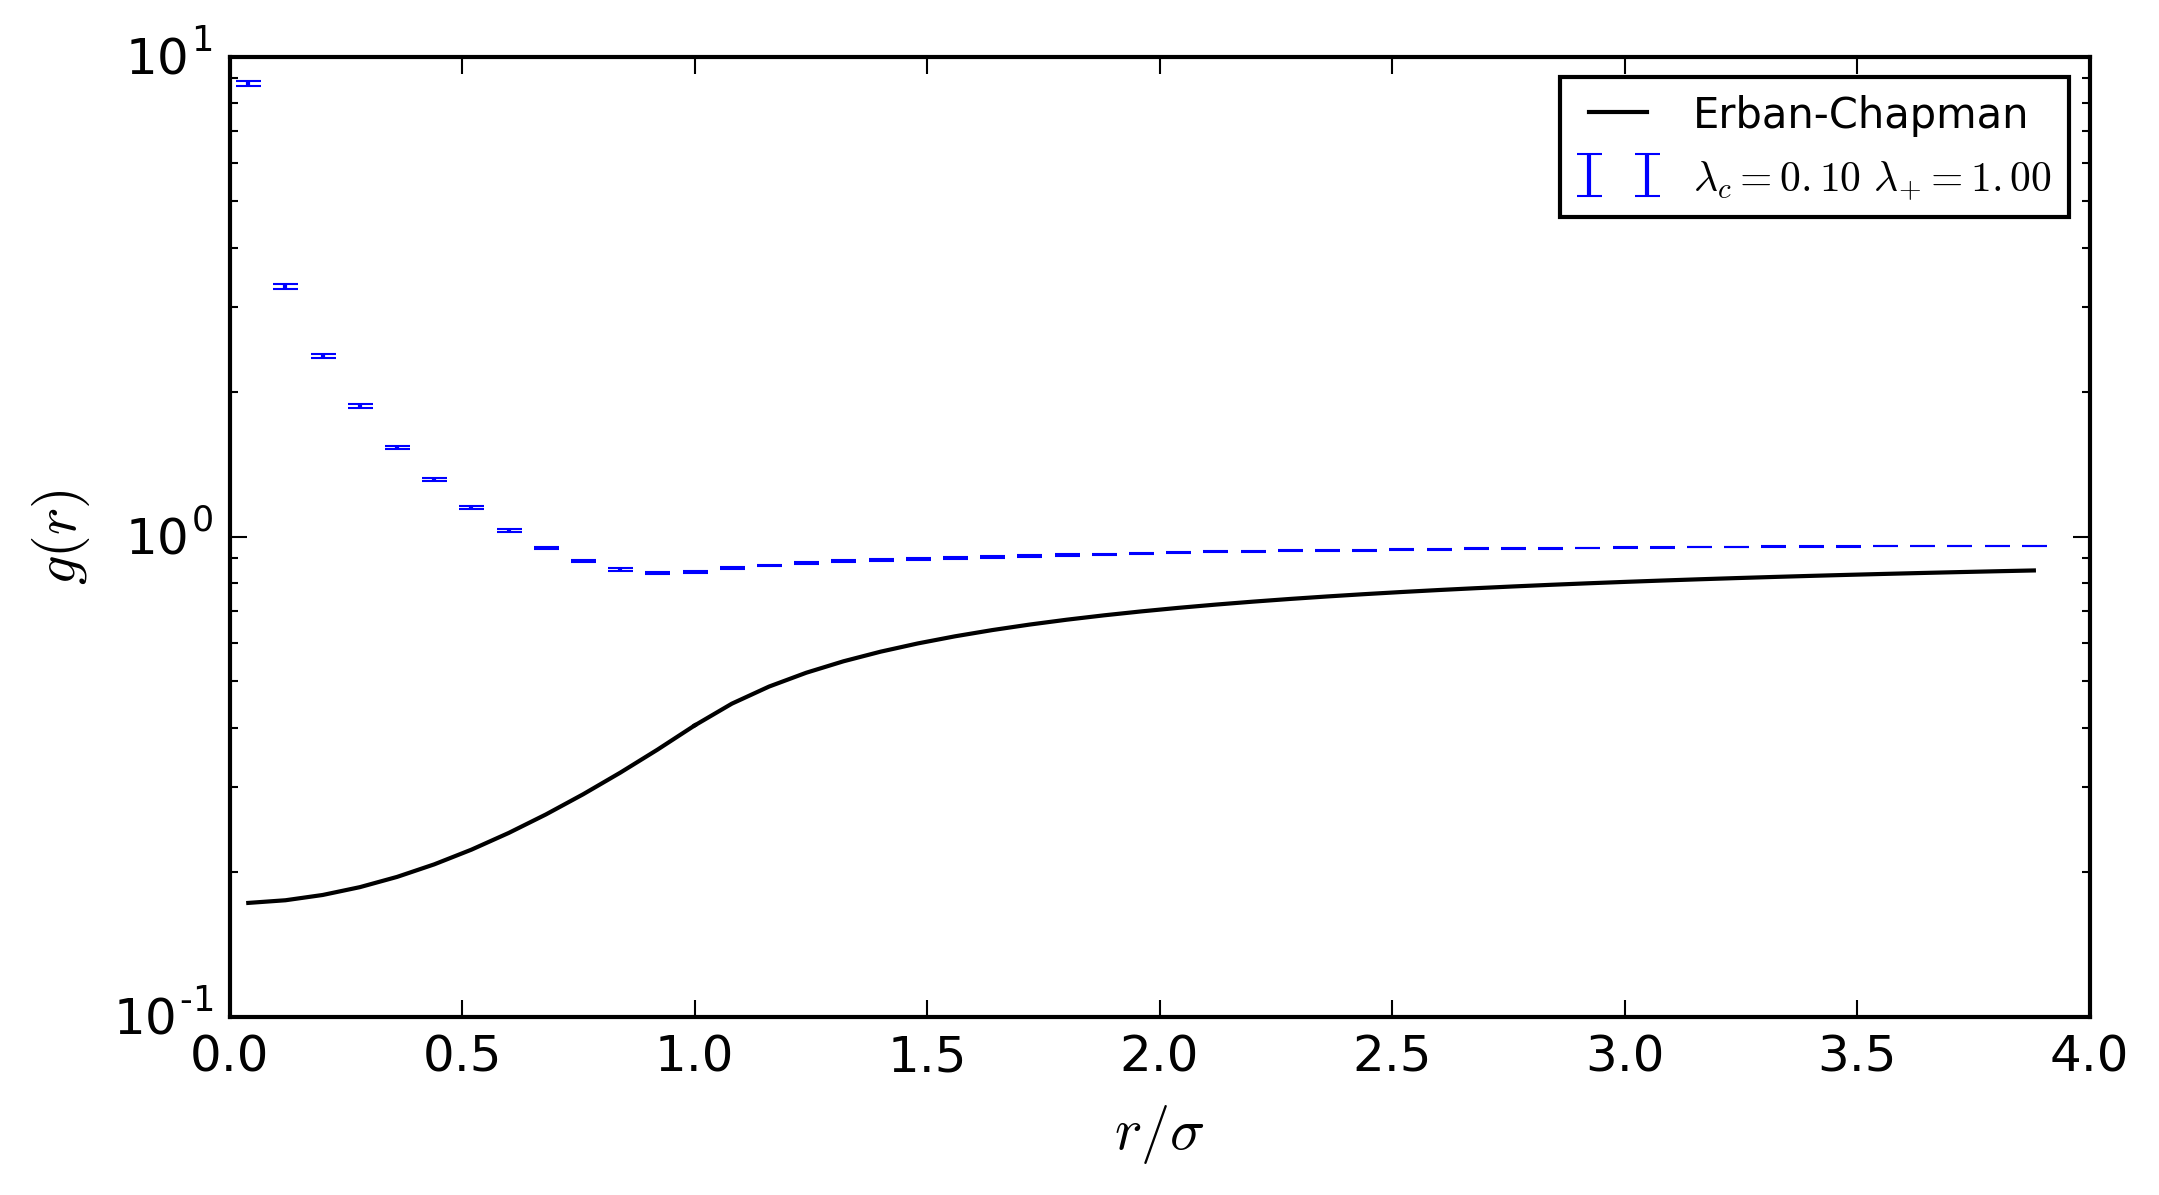
\includegraphics[width=\textwidth]{./data/limit-radial-highlocalconcentration.png}
  \captionsetup{width=\linewidth}
  \captionof{figure}{The radial distribution function of the substrates around the enzyme / complex was observed for $5<t<900$ and plotted as a blue line with an error-bar of the standard deviation. The Erban-Chapman result was plotted as a green dashed line for bigger than the reaction radius $\sigma$  and a red dashed line for smaller than $\sigma$. Parameters were set to:  $\lambda_+=1.0$, $\lambda_-=1.0$,  $\lambda_c=0.1$ and the box size $l^3=8^3$.}
  \label{fig:diffusion1_limit-radial_local concentration}
\end{figure}

\begin{figure}
  \centering
  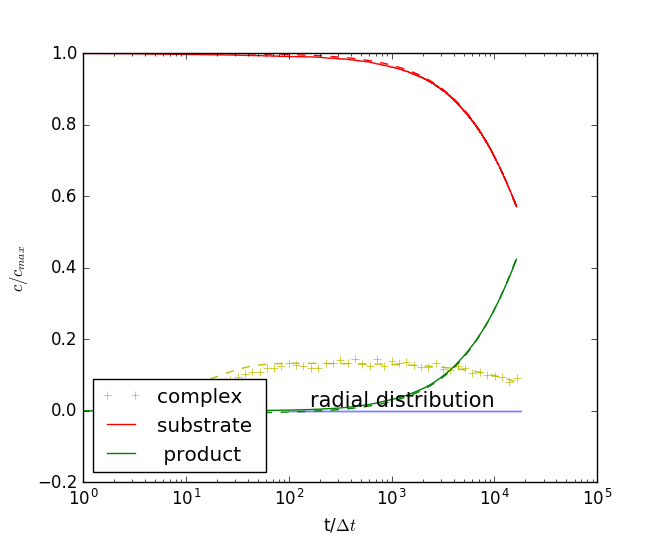
\includegraphics[width=\textwidth]{./data/highlocaldensityconcentrationslin.png}
  \captionsetup{width=\linewidth}
  \captionof{figure}{ Normalized concentrations of substrate, product and complex and their fit with the quasi-steady state approximation for the substrate concentration are shown. The blue bar in the plot indicates the area where the radial distribution was observed, which is plotted in \cref{fig:diffusion_limit-Erban-Chapmann_radial}. The remaining Parameters were set to:  $\lambda_+=1$, $\lambda_-=1$,  $\lambda_c=0.1$ and the box size $l^3=8^3$.}
  \label{fig:enzyme_blocking}
\end{figure}

\begin{comment}
 


\begin{figure}
  \centering
  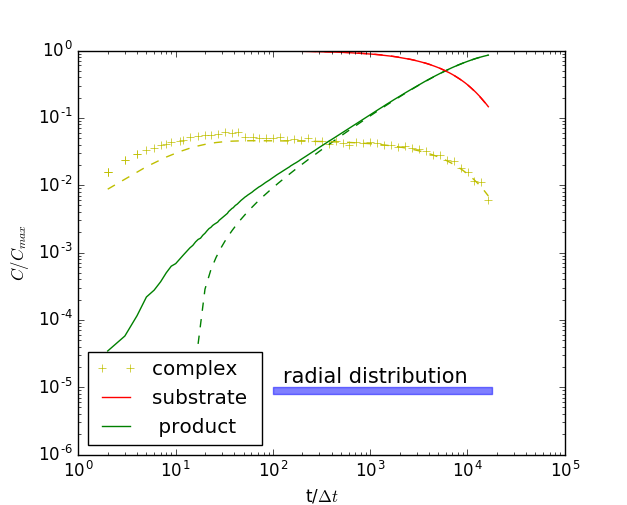
\includegraphics[width=\textwidth]{./data/normal-scenario-concentrations.png}
  \captionsetup{width=\linewidth}
  \captionof{figure}{ Normalized concentrations of substrate, product and complex and their fit with the quasi-steady state approximation for the substrate concentration are shown in the loglog plot. The blue bar in the plot indicates the area where the radial distribution was observed, which is plotted in \cref{fig:diffusion_limit-Erban-Chapmann_radial}. Parameters were set to:  $\lambda_+=1$, $\lambda_-=1$,  $\lambda_c=1.0$ and the box size $l^3=8^3$.}
  \label{fig:normalscenario_reaction}
\end{figure}
averaged over 8700 runs
\end{comment}
\newpage
\begin{comment}
\newpage
\begin{figure}
  \centering
  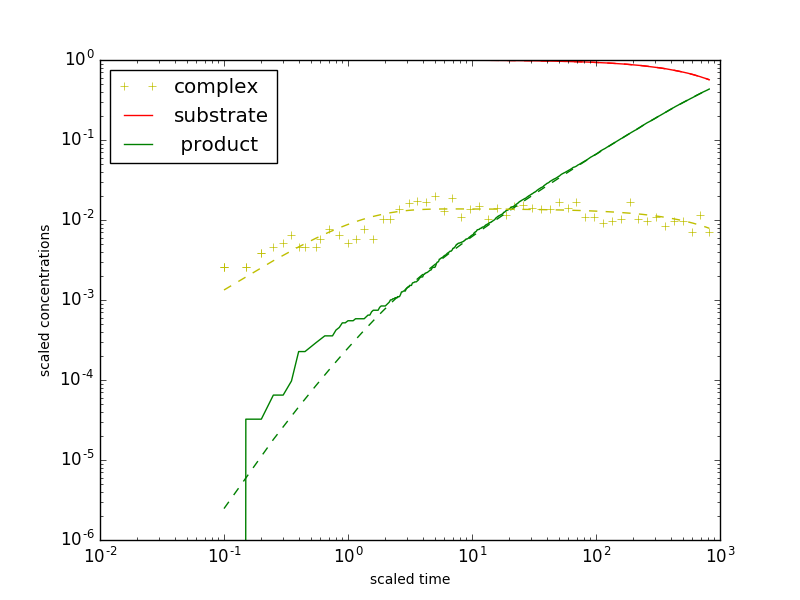
\includegraphics[width=\textwidth]{./data/erban-chapman-limit-concentrations1.png}
  \captionsetup{width=\linewidth}
  \captionof{figure}{ Erban Chapmann Concentrations}
  \label{fig:diffusion_limit-Erban-Chapmann}
\end{figure}
\begin{figure}
  \centering
  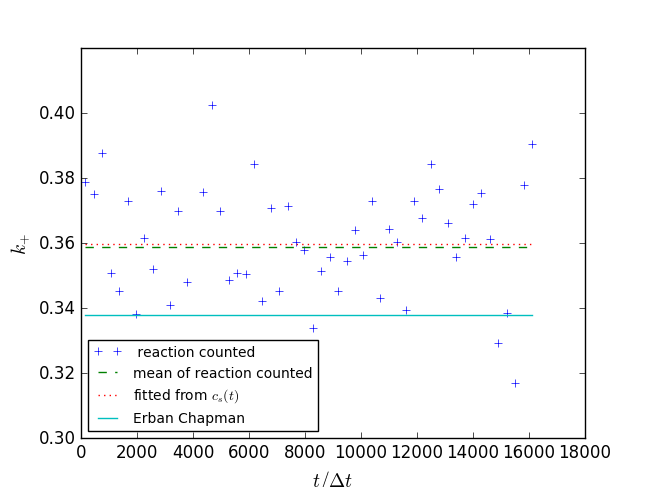
\includegraphics[width=\textwidth]{./data/chapman-limit-concentrations1_k1.png}
  \captionsetup{width=\linewidth}
  \captionof{figure}{ Erban Chapmann $k1$}
  \label{fig:diffusion_limit-Erban-Chapmann_k1}
\end{figure}
\end{comment}
\begin{comment}
\begin{figure}
  \centering
  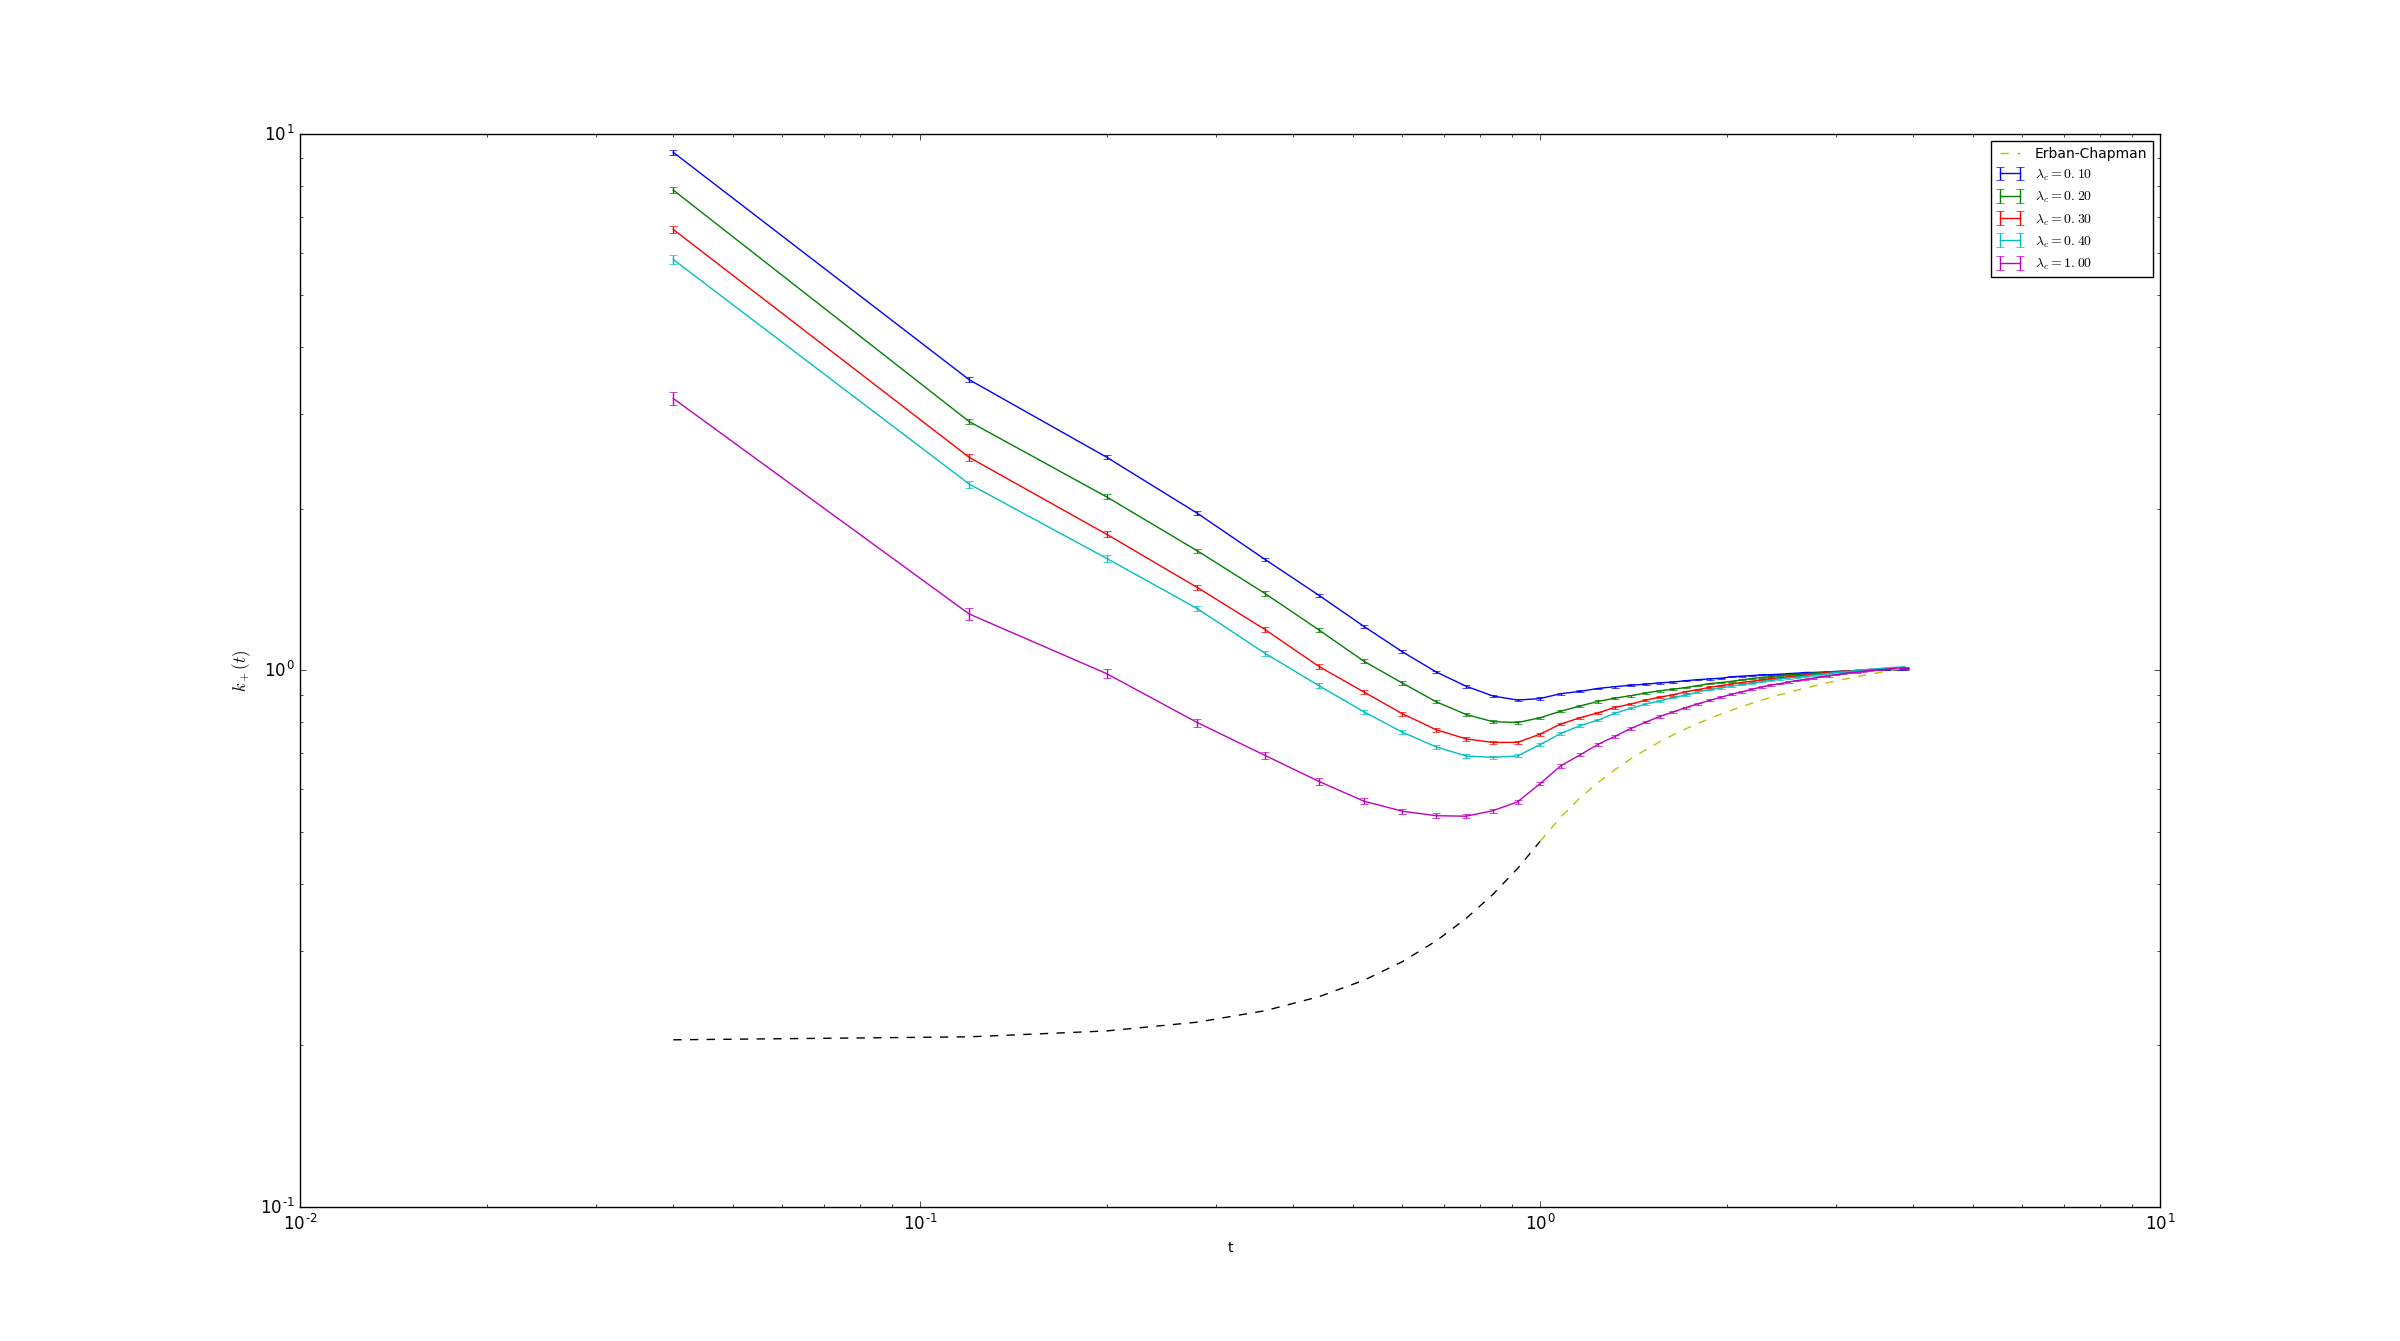
\includegraphics[width=\textwidth]{./data/microrate_complex_radial_erban.png}
  \captionsetup{width=\linewidth}
  \captionof{figure}{ Radial distribution for differnt $k_{c}$ }
  \label{fig:microrate_complex_radial_erban}
\end{figure}
\newpage

\begin{figure}
  \centering
  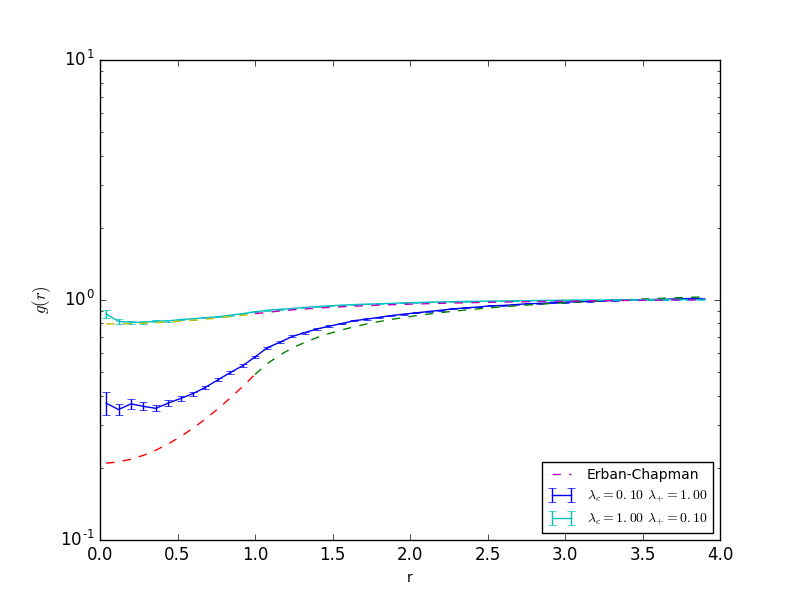
\includegraphics[width=\textwidth]{./data/microrate_complex_vsmicrorate_forward_radial_erban.png}
  \captionsetup{width=\linewidth}
  \captionof{figure}{ Radial distribution for $\lambda_{-}=0$ }
  \label{fig:microrate_complex_vsmicrorate_forward_radial_erban}
\end{figure}
\newpage

\newpage
\begin{figure}
  \centering
  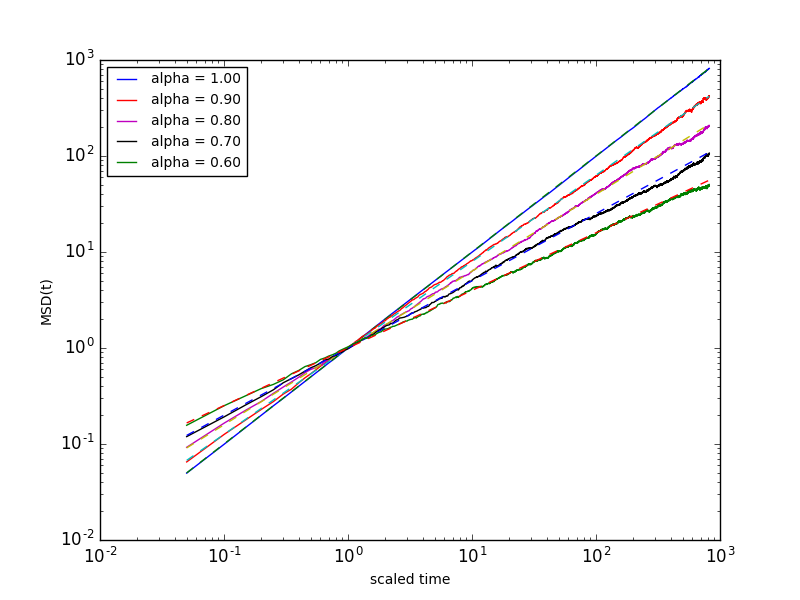
\includegraphics[width=\textwidth]{./data/differentalphamsdrevreaddy.png}
  \captionsetup{width=\linewidth}
  \captionof{figure}{ different alpha}
  \label{fig:differentalpharevreaddymsd}
\end{figure}
\end{comment}
\section{Results for fBm}
The mass action law does not hold anymore for reactions with fractional Brownian motion. Kopelman suggested for percolation cluster, in which particles diffuse   anomalously, to have time depended macroscopic reaction rates for bi-molecular reaction of the form \cite{Kopelman1988}:
\begin{align} \label{ktime}
k(t)=k_0 t^{-h} \qquad \text{for} \qquad 0 \leq h \leq 1 \qquad \text{and} \qquad t \geq 1
\end{align}
to do: check how anomalous diffusion is related to fractal like kinetics factor $h$ \cref{fig:k1differentalphawithfitbetter}. Can be shown that k(t) indeed describes the kinetics of MM with fractional Brownian motion. 

\begin{comment}
 
\begin{figure}
  \centering
  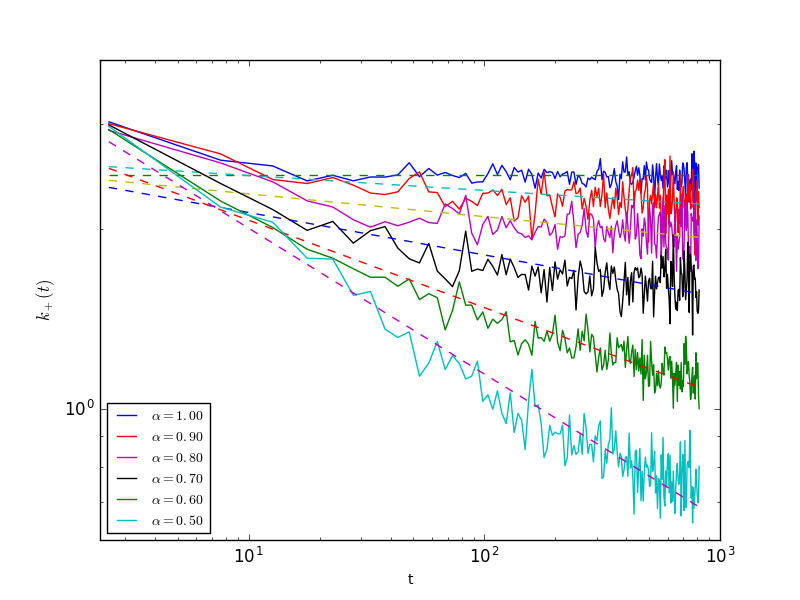
\includegraphics[width=\textwidth]{./data/k1_fordifferentalpha_withfit.png}
  \captionsetup{width=\linewidth}
  \captionof{figure}{$k1(t)$ for different $\alpha$ with fitted h}
  \label{fig:k1differentalphawithfit}
\end{figure}
\end{comment}
\begin{figure}
  \centering
  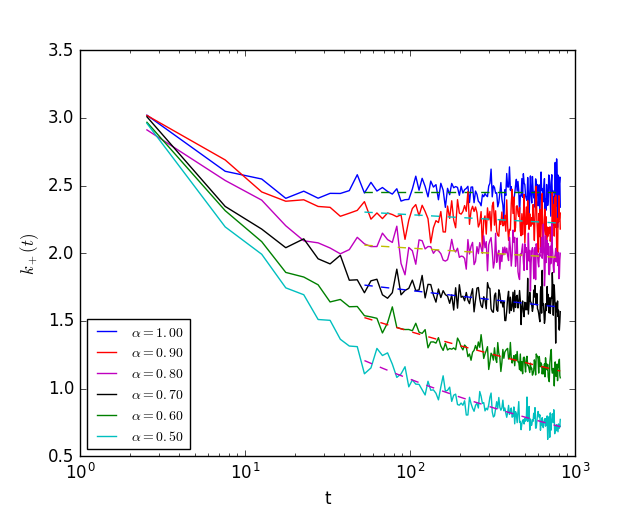
\includegraphics[width=\textwidth]{./data/fractionalalphachangek1.png}
  \captionsetup{width=\linewidth}
  \captionof{figure}{Form the number of reactions $k_{+count}(t)$ was calculated via  \cref{reactioncount} and displayed as solid lines for $0.5\leq\alpha\leq1.0$. With\cref{ktime} the fractal like kinetics exponent $h$ was fitted and displayed as dashed lines in the plot. The remaining parameters were set to: $\lambda_+=1.0$, $\lambda_-=1$,  $\lambda_c=1.0$ and the box size $l^3=8^3$.}
  \label{fig:k1differentalphawithfitbetter}
\end{figure}

\newpage
\section{Conclusion}
The simulation model is capable of reproducing Smoluchwoskis and Erban-Chapman theoretical results for a Bi-molecular reaction. 
The simulation model can be described by Michaelis Menten kinetics for the quasi steady state approximation for normal diffusion but not for anomalous diffusion.
Michaelis Menten reactions in a diffusion controlled regime with fractional Brownian motion are of fractal type. The modeling of biological reaction-diffusion dynamics with fBm can be interesting in a large system with a high number of particles not involved in the reaction mechanism but a small number of reactants, which diffuse anomalously. The large number of particles not  have to be simulated explicitly. There influence on diffusion of the reactants is incorporated in fBm. The missing particle-particle interactions might get negligible with a low density of particles.  
\chapter{Summary}

Cholesky, Davis Harte, our naive and Lowen algorithm for fractional Brownian motion have been implemented and analyzed in terms of accuracy and performance. Our implementation of Lowens algorithm turned out not to be exact as claimed by the author. Davis-Harte method turned out to be both exact and fast $\mathcal{O}(M log(M))$ with $M$ the trajectory length. Davis-Harte and Lowen method was implemented in RevReaDDy. Besides the implementation of fBm many modifications to RevReaDDy were done to deal with our set of questions. A new reaction type and new observables were implemented. Some old observables were modified. A simulation setting with one enzyme and 20 randomly distributed substrates for the Michaelis Menten mechanism was set up and studied under normal Brownian motion and under fractional Brownian motion. Theoretical results from the Smoluchwoski problem of a diffusion controlled bi-molecular reaction and theoretical results for a bi-molecular reaction with microscopic reactions within close proximity to the enzyme could be reproduced by the simulation. It could be shown that the quasi steady-state assumption is indeed reproducing the kinetics of the Michaelis Menten mechanism for our setting, although this approach is not considering a non uniform spatial distribution.\par For fractional Brownian motion with $\alpha<1$ and  $t<1$ a general slowing down of reactions compared to normal diffusion was shown. Reaction rates are time depended for MM with fBm if reaction speed is controlled by diffusion, as Kopelman suggested for particles performing reactions in a percolation cluster ($k(t)=k_0 t^{-h}$). The kinetics are of fractal type.  \par
As an outlook of the thesis a mathematical model for fractal Brownian motion and Michaelis menten mechanism for 3D could be developed. FBm with forces could be studied. Although a algorithm with possible potentials included will probably be very slow. \begin{comment}
outlook:
''''''''''''''''''''''''''''''''''''''''''''
0.find analytical solution to RDPB with brownian motion (chemical lagevin equation?)
besides smoluchswskis PDE, concentration based models.
%http://scitation.aip.org/docserver/fulltext/aip/journal/jcp/113/1/1.481811.pdf?expires=1481129009&id=id&accname=2120797&checksum=758284E4BA8FBF60E006DFB8857194A9

1.find analytical solution to fractional description. (fractional PDE, fraction ODE, fractional master equation,fractional RDME, fractional chemical lagevin equation,  
 fractional master equation fractional diffusion equation %http://www.hrpub.org/download/201308/ms.2013.010208.pdfhttp://www.hrpub.org/download/201308/ms.2013.010208.pdf)
 Fractional master equation and fractal time random walks
 %https://www.icp.uni-stuttgart.de/~hilfer/publikationen/pdfo/PRE-1995-51-R848.pdf
 
2.introduce forces (complicated)

2.1 find analytical solution

3. find similar time depended reaction rates with interaction potentials, obstacles and Brownian dynamics (interesting for presentation, first this simulation with mean square displacement. then let all the other particles vanish and fbm is performed. on the side msd is shown simultaneous how it develops.problem no excluded volume but not so important cause, small abundances are especially interesting.)
''''''''''''''''''''''''

Outlook in two section
1: scientifically interesting :
-introduce forces (complicated) and find find analytical solution
-find analytical solution to RDPB with brownian motion (chemical lagevin equation?) besides smoluchswskis PDE, concentration based models.
- Fractional master equation and fractal time random walks


2:interesting for integration as an modeling tool:
-not only fBm but any velocity correlation function measured by n experiment
-introduce forces (complicated)
-verify by finding similar time depended reaction rates with interaction potentials, obstacles and Brownian dynamics 
\end{comment}
 
 
\chapter{Appendix}
\section{From Central Limit Theorem to Gaussian Distribution}\label{append:CLT}
In the following the Central Limit Theorem will be applied to calculated the distribution of Y,  $\rho(y)dy=P(y<Y<y+dy)$ in the limit of large N , with Y being defined as the sum of an random variable:
 \begin{align}
  Y = \frac{1}{\sqrt{N}} \sum_{j=1}^N X_j \label{eq:CLT1}
 \end{align}
The Generating function for a random variable $Y$ is: 
\begin{align}
 G_Y(k)=\langle e^{ikY}\rangle = \int e^{ikY} \rho(y)dy
\end{align}
\cref{eq:CLT1} can be inserted into the generating function, which results in:
\begin{align*}
G_Y(k)=\langle e^{\frac{ik}{\sqrt{N}} \sum_{j=1}^N X_j}\rangle \\
G_Y(k)=\langle \prod_{j=i}^N e^{\frac{ik}{\sqrt{N}} X_j} \rangle 
\end{align*}
If all $X_j$ are independent, then:
\begin{align}
 G_Y(k)= \prod_{j=i}^N \langle e^{\frac{ik}{\sqrt{N}} X_j} \rangle =e^{\sum_{j=1}^N A_j (\frac{k}{\sqrt{N}})} \\ \nonumber \text{ with } A_j(\frac{k}{\sqrt{N}})= ln \langle e^{\frac{ik}{\sqrt{N}} X_j} \rangle 
\end{align}
For large N behavior, we assume $\frac{k}{\sqrt{N}} << 1$ and expand
\begin{align}
 A_j(\frac{k}{\sqrt{N}}) = ln(1+ \langle X_j \rangle \frac{ik}{\sqrt{N}} - \langle X_{j}^2 \rangle \frac{k^2}{2N}+\mathcal{O}(N^{- \frac{3}{2}}))
\end{align}
 with a finite variance $ \sigma_i^2=\langle X_{i}^2\rangle $ and the mean $\langle X_{i}\rangle = 0$
\begin{align}
 A_j(\frac{k}{\sqrt{N}}) = -\sigma_j^2 \frac{k^2}{2N}+\mathcal{O}(N^{- \frac{3}{2}}))
\end{align}

Thus, the generating function for large N is:

\begin{align}
 G_Y(k)=e^{- \frac{\sigma^2 k^2}{2}} \\ \nonumber
 \text{ with } \sigma =  \frac{1}{N} \sum_{j=1}^N \sigma_j^2 
\end{align}
The distribution of Y can be calculated via the inverse Fourier Transform:
\begin{align}
 \rho(y) &=\frac{1}{2 \pi} \int_{-\infty}^{\infty} e^{- \frac{\sigma^2 k^2}{2}} e^{i k y} dk \\  
 &=\frac{1}{\sqrt{2 \pi} \sigma } e^{-\frac{y^2}{2 \sigma^2}}
\end{align}
$\rho(y)$ results in a Gaussian distribution.

\section{From Gaussian Distribution to Gaussian Transition Probability}\label{baystheorem}
The conditional distribution function to be in $x$ at time $t$ if visited position $y$ at time $s$   can be written due to Bayes' theorem as a transition probability from $y$ to $x$ in time $t-s$ multiplied with the probability to be in $y$ at time $s$:
\begin{align}
 \rho_{t,s}(x,y)=T_{t-s}(x|y) \rho_s(y)
\end{align}
Further due to particle conservation another relation holds:
\begin{align}
 \rho_{t}(x)= \int \rho_{t,s}(x,y) dy
\end{align}
Having an initial condition $\rho_{s}(x)= \delta(x-y)$:
\begin{align}
 \rho_{t,s}(x|y)&= \int \rho_{t,s}(x,y) dy = \int T_{t-s}(x|y) \rho_s(y) dy\\
 &= \int T_{t-s}(x|y) \delta(x-y) dy 
 = T_{t-s}(x|y)
\end{align}
\section{Einstein Formula} \label{einsteinrealtionappendix}
The derivative of the mean variance of the Gaussian distribution in respect to time is defined as:
\begin{align}
 \frac{d}{dt}  \delta \bm{r}^2(t)&=\frac{d}{dt} \langle \Delta \bm{ R}^2(t)\rangle  =\frac{d}{dt} \int d\bm{r} \bm{r}^2 c(\bm{r},t)=\int d\bm{r} \bm{r}^2 \frac{\partial}{\partial t} c(\bm{r},t) 
\end{align}
Fick's second law can be applied:
\begin{align}
&= D \int_{-\infty}^{\infty}d\bm{r} \bm{r}^2 \Delta c(\bm{r},t)  
\end{align}
Assuming a reasonable assumption  $c(\pm \infty,t)=0$  and two times partial integration one can derive:
\begin{align}
&= -2 D \int_{-\infty}^{\infty} d\bm{r} \bm{r} \nabla c(\bm{r},t) \\ &= 2 D d \int_{-\infty}^{\infty} d\bm{r} c(\bm{r},t) =2dD
\end{align}
For the initial condition $\bm{r}(0) = 0$,  one gets the Einstein Formula: $\langle (\bm{r}(t)-\bm{r}(0))^2)\rangle= 2dDt$
\begin{comment}
check book zwanzig

\section{Power spectral density for fGn}\label{VACF}
The power spectral density function can be calculated from the Wiener-Khinchin theorem as the Fourier transform the auto-covariance function. The auto-covariance function for ctfGn can be derived from fractional Brownian motion:
\begin{align}
\mathrm{Cov}[X^{\alpha}_t,X^{\alpha}_0]&=\sigma^2 \frac{d^2 |t|^{\alpha}}{dt^2}\\
\end{align}
The power spectral density can be written as the Fourier transform of the auto-covariance function:
\begin{align}
 S(\omega)&= \int^{\infty}_{-\infty} \mathrm{Cov}[X^{\alpha}_t,X^{\alpha}_0] \exp[-2 \pi i \omega t] dt\\
 &=\int^{\infty}_{-\infty} \sigma^2 \frac{d^2 |t|^{\alpha}}{dt^2} \exp[-2 \pi i \omega t]=2 \sigma^2  \int^{\infty}_{0} \frac{d^2 |t|^{\alpha}}{dt^2} \exp[-2 \pi i \omega]
\end{align}
With partial integration one arrives at:
\begin{align*}
  \stackrel{par. integ.}{=}2 \sigma^2 \left( \underbrace{\left [ \exp[-2 \pi i\omega t] \frac{d}{dt} t^{\alpha} \right]_{0}^{\infty}}_{\stackrel{\alpha < 2} {=} 0}+ i \omega \int_{0}^{\infty} d t e^{-2 \pi i \omega t} \left[\frac{d}{dt}t^{\alpha} \right] \right) 
 \end{align*}
Partial integration and Tauber theorem yields:

\begin{align*}
  &\stackrel{par. integ.}{=}2 \sigma^2 \left( \underbrace{\left [ \exp[-2 \pi i\omega t]  t^{\alpha} \right]_{0}^{\infty}}_{\stackrel{\alpha < 1} {=} 0}+ (i \omega)^2 \int_{0}^{\infty} d t e^{-2 \pi i\omega t} \left[ t^{\alpha} \right] \right) \\
  &= \sigma^2 \Gamma(1+\alpha)(i \omega)^{1-\alpha} \qquad \text{for} \qquad \alpha < 1
\end{align*}
\end{comment}

\section{Erban-Chapman}\label{Erban-Chapmann}
The calculation can be started from \cref{smoluchwoskionedimension}. This derivation can be found in \cite{Erban2009}. The stationary distribution can be written as:
\begin{align}
\left(\frac{\partial}{\partial_r}+\frac{2}{r} \right) D \frac{\partial\rho_t(r)}{\partial_r}=0 \qquad \text{for} \qquad r \geq \sigma \\
\left(\frac{\partial}{\partial_r}+\frac{2}{r} \right) D \frac{\partial\rho_t(r)}{\partial_r}=\lambda_{+} \rho_t(r)  \qquad \text{for} \qquad r \leq \sigma
\end{align}
For  $r \leq \sigma$ a production term had been added to the continuity equation. The general solution can be written as: 
\begin{align}
\rho_t(r)= a_1+\frac{a_2}{r} \qquad \text{for} \qquad r \geq \sigma \label{erbanchapmanradial1} \\
\rho_t(r)= \frac{a_3}{r} \exp \left[ r \sqrt{\frac{\lambda_{+}}{D}} \right] + \frac{a_4}{r} \exp \left[-r \sqrt{\frac{\lambda_{+}}{D}} \right] \qquad\text{for}\qquad r \leq \sigma \label{erbanchapmanradial}
\end{align}
with $a_1, a_2, a_3, a_4$ real constants. Just like in the calculation in diffusion limit the distribution at  $r \rightarrow \infty$ is defined as the concentration of particle A $\rho_t(r \rightarrow \infty)=C_A$. Thus $a_1=C_A$ and due to the continuity of the density distribution , $a_3=-a_4$. Further, due to the continuity of the the flux $j_s(r)$ at $r=\sigma$ also $a_2$ and $a_3$ can be determined:
\begin{align}
 a_2&= C_A \left( \sqrt{\frac{D}{\lambda_{+}}} \tanh\left(\sigma \sqrt{\frac{\lambda_{+}}{D}}\right)-\sigma\right)  \\
 a_3&= \frac{C_A  \sqrt{\frac{D}{\lambda_{+}}}}{2 \cosh\left(\sigma \sqrt{\frac{\lambda_{+}}{D}}\right)}
\end{align}
The flux at  $r= \sigma$ can be written as:
\begin{align}
j^{s}(\sigma)=D \frac{\partial\rho_t(\sigma)}{\partial_{\sigma}}= -D \frac{a_2}{\sigma^2} 
\end{align}
Gauss's theorem states that the negative flux of a quantity through a closed surface is equal to the production of that quantity inside the volume. Further The change of complex AB is proportional to the change of A inside the volume of of the sphere with $r=\sigma$. The total flux and thus the change of AB can be written as:
\begin{align}
  \frac{d C_{AB} }{dt}&=- \int_{\partial V} j^{s}(\sigma) da= \int_{\partial V} D \frac{a_2} {\sigma^2}  da =- 4 \pi D a_2 C_B \\ &= 4 \pi D C_B  C_A \left(\sigma -\sqrt{\frac{D}{\lambda_{+}}} \tanh\left(\sigma \sqrt{\frac{\lambda_{+}}{D}}\right)\right)
\end{align}



\begin{comment}
 

\section{Kinetics of the Bi-Molecular Chemical Reaction in Solution}\label{bi-molecular}
The aim of this calculation is to derive the kinetics for the following reaction scheme: \ch{A + B <=>[ $k^{+}_{\mathrm{d}}$ ][ $k^{-}_{\mathrm{d}}$ ] AB }\newline
The derivation is calculated under the assumption of free diffusion of particle A and B with the diffusion constants $D_A$ and $D_B$ , respectively and without any interactions between them. 
The joint concentration field can be described by the Smoluchowski equation for a bi-molecular system in a solution:
\begin{align}
 \frac{\partial \rho_t(\bm{r}_A,\bm{r}_B)}{\partial t}=(D_A \nabla^{2}_{A}+D_B \nabla^{2}_{B}) \rho_t(\bm{r}_A,\bm{r}_B) \label{smolubi}
\end{align}
The complexity of the problem can be reduced by substituting the positions of the particles A and B with their relative distance $\bm{r}=\bm{r}_A-\bm{r}_B$. It is convenient to introduce even further substitutions:
\begin{align}
 D= D_A+D_B \qquad \qquad \bm{R}=\frac{D_B \bm{r}_A+ D_A \bm{r}_B}{D_A+D_B}
\end{align}
the Laplace operator in terms of new coordinates result in:
\begin{align}
\nabla^{2}_{A} = \left( \nabla_r+\frac{D_B}{D} \nabla_R \right)^2 \\
\nabla^{2}_{B} = \left( \nabla_r+\frac{D_A}{D} \nabla_R \right)^2 
\end{align}
Inserting these in \cref{smolubi} one gets:
\begin{align}
 \frac{\partial \tilde{\rho}_t(\bm{r},\bm{R})}{\partial t}=\left(D \nabla^{2}_{r}+\frac{D_B D_A}{D_A+D_B}\nabla^{2}_{R}\right) \tilde{\rho}_t(\bm{r},\bm{R})
\end{align}
The equation is describing two independent diffusion processes, one in
the coordinate $\bm{r}$ and one in the coordinate $\bm{R}$. The solution can be obtained by the product ansatz $\tilde{\rho}_t(\bm{r},\bm{R})=\rho_t(\bm{r})q_t(\bm{R})$. Integration over $\bm{R}$ results in:
\begin{align}
\frac{\partial \rho_t(\bm{r})}{\partial t}=D \nabla^{2}_{r} \rho_t(\bm{r}) +\frac{D_B D_A}{D_A+D_B} \nabla^{2}_{R} \rho_t(\bm{r}) \int_{\partial V} q_t(\bm{R}) d \bm{a}
\end{align}
In the previous equation the stokes theorem was applied. The second term is zero due to conservation of probability. The problem is isotropic, hence $r=|\bm{r}|$ and $\nabla^{2}_{\bm{r}}=\left(\partial_r+\frac{2}{r}\right)\partial$. The equation reduce to one dimension:
\begin{align}
\frac{\partial \rho_t(r)}{\partial t}=-\left(\frac{\partial}{\partial_r}+\frac{2}{r} \right) j_t(r) \qquad \qquad j_t(r)=D \frac{\partial\rho_t(r)}{\partial_r}
\end{align}
 The stationary distribution results in:
\begin{align}
 0 &=-\left(\frac{\partial}{\partial_r}+\frac{2}{r} \right) j^{s}_t(r) \\
 \frac{d j^{s}_t(r)}{j^{s}_t(r)}  &=- \frac{2}{r} dr\\
 j^{s}_t(r)&=A r^{-2}\\
 \rho^s(r)&=\rho^s(r_0)- \frac{\int_{r_0}^{r} j^{s}_t(r')dr'}{D}=\rho^s(r_0)+\frac{A}{D}\left(\frac{1}{r}-\frac{1}{r_0}\right)
\end{align}
Now assuming only a single B molecule being at the position $r=0$. Instantaneous reaction occur for $r\leq \sigma \Rightarrow \rho_t(r \leq \sigma)=0$. For $r \rightarrow \infty$ the distribution is than defined as the concentration of particle A $\rho_t(r \rightarrow \infty)=c_A$ and 
the Solutions for $\rho^{s}(r)$ and $j^{s}_t(r)$ for the boundary conditions are:
\begin{align}
 \rho^{s}(r)=C_A \left(1-\frac{\sigma}{r}\right) \qquad j^{s}_t(r)&=-D \sigma C_A r^{-2}
\end{align}
The change of the concentration of $C_{AB}$ is then: 
\begin{align}
 \frac{d C_{AB} }{d}=4 \pi \sigma D C_A C_B
\end{align}
By formulating the problem in relative distance from particle A and B. It was also reasonable to keep particle B at its initial position. The results shows the relation between the product of the concentrations and the concentration change.In the derivation of Michealis-Menten kinetics this is an assumption. 


\end{comment}

\section{Michaelis-Menten Kinetics}\label{Menten_der}
Michaelis-Menten kinetics are describing the following reaction: \par
\ch{S + E <>[ $k_{\mathrm{+}}$ ][ $k_{\mathrm{-}}$ ] E S -> [ $k_{\mathrm{c}}$ ] P + E}.
A set of differential equations can be formulated as a result of mass conservation and the mass action law:
\begin{align}
\frac{dc_P(t)}{dt} &= k_{\mathrm{c}} c_{ES}(t) \\ \label{first}
\frac{dc_E(t)}{dt} &= k_{\mathrm{c}} c_{ES}(t)+k_{\mathrm{-}} c_{ES}(t)-k_{\mathrm{-}} C_E(t) C_S(t)\\
\frac{dc_S(t)}{dt} &= k_{\mathrm{-}} c_{ES}(t)-k_{\mathrm{+}} c_E(t) c_S(t)\\
\frac{dc_{ES}(t)}{dt} &=  - k_{\mathrm{c}} c_{ES}(t) -k_{\mathrm{-}} c_{ES}(t)+k_{\mathrm{+}} c_E(t) c_S(t) \label{quasisteadymichaelis}
\end{align}
With a quasi-steady-state approximation: $\frac{dc_{ES}(t)}{dt}=0$ one can reduce label{quasisteadymichaelis} to: $ k_{\mathrm{+}}c_E(t) C_S(t)=k_{\mathrm{-}}c_{ES}+k_{\mathrm{c}}c_{ES}(t)$. A Rearrangement of this equation results in the Michaelis-Menten constant:
\begin{align}
 K_M=\frac{k_{\mathrm{-}}+k_{\mathrm{c}}}{k_{\mathrm{+}}}=\frac{c_E(t) c_S(t)}{c_{ES}}. 
\end{align}
From mass conservation law one gets: $c_E(t)=c_{E_0} -c_{ES}(t) $
After inserting this equation into the quasi-steady-state approximation of \cref{quasisteadymichaelis}, one gets:
\begin{align}
 c_{ES}(t)=\frac{c_{E_0} c_S(t)}{K_M+c_S(t)}
\end{align}
The combination of this eq. with the first differential \cref{first} defines the velocity of the reaction:
\begin{align}
 v(c_S(t))= \frac{dc_P(t)}{dt}= k_{\mathrm{c}} \frac{c_{E_0} c_S(t)}{K_M+c_S(t)} = v_{max} \frac{c_S(t)}{K_M+c_S(t)}  
\end{align}

\begin{comment}
 

\chapter{old stuff}
\section{Theory}
\subsection{Diffusion-controlled Reactions for Brownian Motion}
Chemical reactions are omnipresent in biological systems. Reactions are composed of reactants and products. These reactants and products are atoms or molecules with changing number over time during reactions. Studying chemical reactions often contains reaction kinetics. Reaction kinetics is about rates of chemical process. Enzymatic reactions e.g. play an important role in biological systems to reduce rates of reactions. The rates of reactions in solutions are not only governed by intrinsic reaction rates, which were addressed e.g. by Kramer's escape problem for two reactants, but also on rates at which the chemical participants diffuse into close proximity. In a reaction of the following type: \ch{A + B <>[ $k^{+}_{\mathrm{d}}$ ][ $k^{-}_{\mathrm{d}}$ ] AB <> [ $k^{+}_{\mathrm{a}}$ ][ $k^{-}_{\mathrm{a}}$ ] C}. \newline The Kramer's escape problem deals with the rates on the right side  $k^{\pm}_{\mathrm{a}}$. Smoluchowski deals with the rates on the other side $k^{\pm}_{\mathrm{d}}$. \newline  A theoretical approach on how fast two particles come together in a dilute system of hard spheres moving independently with Brownian motion have been studied by Marian von Smoluchowski in 1916 \cite{Smoluchowski1}. This was the first study on diffusion-limited reaction rates. A constant rate $k^{+}$ can be written as:
\begin{align}
 k^{+}=4 \pi (D_1+D_2)(R_1+R_2)=4 \pi (D_1+D_2) \sigma \label{reactionrate11}
\end{align}
with $\sigma = R_1+R_2$ the relative distance between the sphere centres.  It is a direct result of the diffusion equation. The calculation can be found in the appendix \ref{bi-molecular}. One particular area of research on which the Smoluchowski relation had significant impact in the last few decades is biology. This is unsurprising as a vast number of biomolecular systems involve dilute and minute diffusing molecular populations undergoing continuous reaction. Understanding how these biological systems operate is complicated and is in itself a whole field of research; systems biology. The Smoluchowski result has provided a very powerful tool for theoretical investigation of microscopic biochemical reaction-diffusion processes \cite{Flegg}. It was extended by P. Debye in 1942 to add intermolecular forces. However, especially in biological systems Brownian motion do not apply for all time-scales. As stated in the motivation these environments exhibit very often anomalous diffusion, which can be addressed by fBm. 
\newline
A related reaction type was studied by L. Michaelis and Maud L. Menten in 1913 \cite{Johnson2011}. Also Known as Michaelis-Menten kinetics:   
\ch{S + E <>[ $k_{\mathrm{1}}$ ][ $k'_{\mathrm{1}}$ ] E S <> [ $k_{\mathrm{2}}$ ] [ $k'_{\mathrm{2}}$ ]P + E}, with $k'_{\mathrm{2}}=0$. The assumption of irreversibility can be considers as a good approximation, if the concentration of the substrate  is a lot larger then the concentration of the Product $[S]\gg[P]$ or if the Gibbs free energy (released energy) is very large  $\Delta G \ll 0$ (Kramer's escape Problem). With a further quasi-steady-state approximation  ($k_{\mathrm{1}}[E][S]=k'_{\mathrm{1}}[ES]+k_{\mathrm{2}}[ES]$) the Michaelis-Menten equation results in:
\begin{align}
 v= \frac{d[P]}{dt}=V_{max} \frac{[S]}{K_M+[S]}  \qquad \text{ with } \qquad K_M=\frac{k'_{\mathrm{1}}+k_{\mathrm{2}}}{k_{\mathrm{1}}}
\end{align}
The derivation can be found in the appendix \ref{Menten_der} . In the first step the relation $\frac{d[ES]}{dt}\propto [E][S]$ is assumed. This is coherent with the results from the calculation for kinetics of bi-molecular reaction in solutions with the assumption of normal diffusion in \cref{bi-molecular}. However, in the environment of a living cell where there is a high concentration of proteins, the cytoplasm often behaves more like a gel than a liquid, limiting molecular movements and altering reaction rates \cite{Zhou2008}.

\begin{comment}
 Belousov-Zhabotinsky-Reaktion ?
 https://en.wikipedia.org/wiki/Reaction%E2%80%93diffusion_system interessint 
 Two-component reaction–diffusion equations

\section{Simulation and Outlook}
A software package revReaDDy was used to simulate reactions in a dilute system. It builds upon ReaDDy \cite{Johannesschoneberg2014} and is still under development. It is a particle based simulation software acting on a macromolecular level. For the following simulation Brownian motion was used as an integrator and will be replaced by fBm in the second half of the master thesis. RevReaDDy has periodic boundary conditions. In the following, possible input parameters will be mentioned.  Particle types with a radius and diffusion constant can be defined. Further, also the simulation box size can be varied. Different types of reactions can be incorporated. Their parameters are: 1. Intrinsic reaction rates $k_a$: They describe the speed of the reaction as soon as the reactants are in a close proximity. 2. The distance for close proximity. 3. Which particles take part in the reaction. \newline In the following, results from an enzymatic reaction will be shown. The reaction is a simplified version of Michaelis-Menten. That is what we intended to simulate. Formation of complexes is still not integrated in revReaDDy. A close reaction scheme to Michaelis-Menten  can be reduced to: \ch{S + E -> [ $k_{\mathrm{1}}$ ] P + E}. This kind of reaction type  is already integrated in ReaDDy and can be used. The concentrations over time for this reaction results in:
\begin{align}
 c_S(t)&=c_{s_0} e^{- t k_1  c_E} \\
 c_P(t)&=c_{s_0}\left(1- e^{-t k_1  c_E}\right)
\end{align}
for boundary conditions $c_P(0)=0$. The intrinsic reaction parameter is set to be infinite so that reactions occur immediately if particles surpass the reaction radius $\sigma$. This setup is completely diffusion limited and \cref{reactionrate11} can be applied. The resulting time dependent  concentrations are:
\begin{align}
 c_S(t)&=c_{s_o} e^{- t 4 \pi (D_1+D_2) \sigma  c_E}  \label{substratetheo}\\
 c_P(t)&=c_{s_0} \left(1- e^{-t 4 \pi (D_1+D_2) \sigma  c_E}\right)
\end{align}
This setup has been simulated with only one enzyme. The time dependent particle number of the substrate  $S(t)$ was recorded for different diffusion constants and compared to the theoretical values. The result can be seen in \cref{fig:reactionssimulation}. The theory is fitting to the exponential decay in the simulation. This simulation shows the influence of $D$ on reactions. 
\begin{figure}[h!]
  \centering
  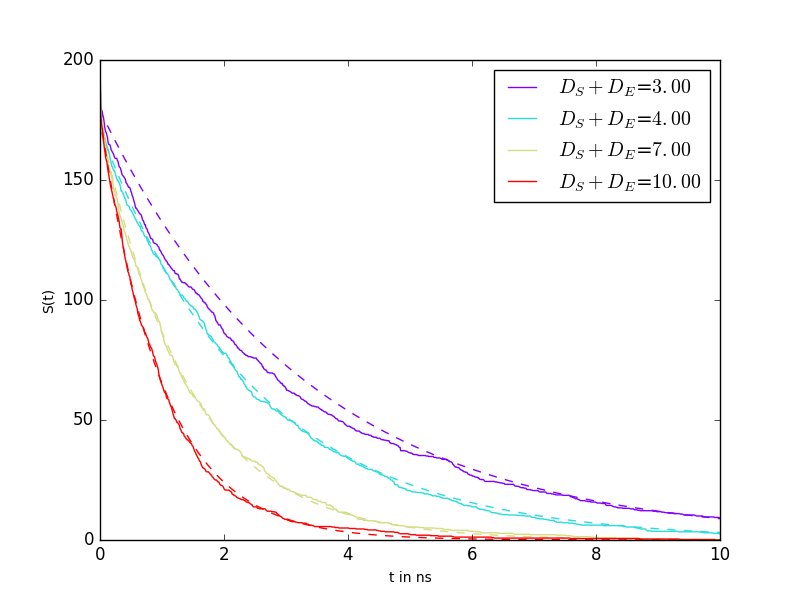
\includegraphics[width=\linewidth]{./data/besta.png}
  \captionsetup{width=0.9\linewidth}
  \captionof{figure}{Substrate particle number $S(t)$ for different Diffusion constants $D$ of the enzyme and substrate. With fitted theoretical curves from equation \cref{substratetheo}. The input parameters for RevReaDDy are: box size$=10^3nm$,reaction distance $=3$,intrinsic reaction rate$=10^{25}$, timesteps$=1000$,$S(0)=300$.}
  \label{fig:reactionssimulation}
\end{figure}
\newline \noindent In the second half of the master thesis fBm is going to be integrated in RevReaDDy. Similar simulations with fBm are going to be studied and related to Brownian motion. Spatial distributions of the reactants are going to be studied. The algorithm for fBm uses his velocity autocorrelation function. In principle it should be possible to integrate also different VACFs. The fBm integrator would result in an more general integrator, which could be used to model environments from real experiments. Including the VACF in the integrator may be an elegant way of adding an approximation due to the experimental environment. 

%\subsection{Code:Gebrochen-rationale Brownische Bewegung}
%\lstinputlisting[language=Python]{../simulation.py}
\end{comment}

\nocite{}

%\printindex
\bibliography{literatur}


\end{document}
